\documentclass[
%paper=5.5in:8.5in,
a5paper,
]{scrbook} 

\usepackage{bindery}
\usepackage{illustrations}
\usepackage{dropcaps}
\usepackage{verse}
\usepackage{chessboard}
\usepackage{adjustbox}



\setdropcaps{Roycroft Initials.ttf}

\makeatletter
\@ifundefined{ifpictures}{\newif\ifpictures}{}
\makeatother
\picturestrue
%\picturesfalse

\ifpictures
    \includecomment{pictures}
    \excludecomment{placeholder}
\else
    \excludecomment{pictures}
    \includecomment{placeholder}
\fi


%\BeforeTOCHead[toc]{%
%  \KOMAoptions{parskip=false}% no parskip in ToC
%  \RedeclareSectionCommand[afterskip=1sp minus 1sp]{chapter}% no skip after ToC title
%}
%\BeforeTOCHead[tocline]{%
%  \KOMAoptions{parskip=false,numwidth=0}% no parskip in ToC
%  \RedeclareSectionCommand[afterskip=1sp minus 1sp]{chapter}% no skip after ToC title
%}


\automark{chapter}
\lehead{Through the Looking-Glass}
\rohead{\leftmark}
\flushbottom


\hyphenation{}

\begin{document}
\frontmatter

%half title
%\vspace*{\fill}
%\begin{center}
%{\chapterfont\Huge Through the Looking-Glass}\\
%\vspace{4em}
%{\chapterfont\Large Lewis Carroll}
%\end{center}
%\thispagestyle{empty}
%\cleardoubleoddpage
\KOMAoptions{headings=openright}

\begin{pictures}
\pagestyle{empty}

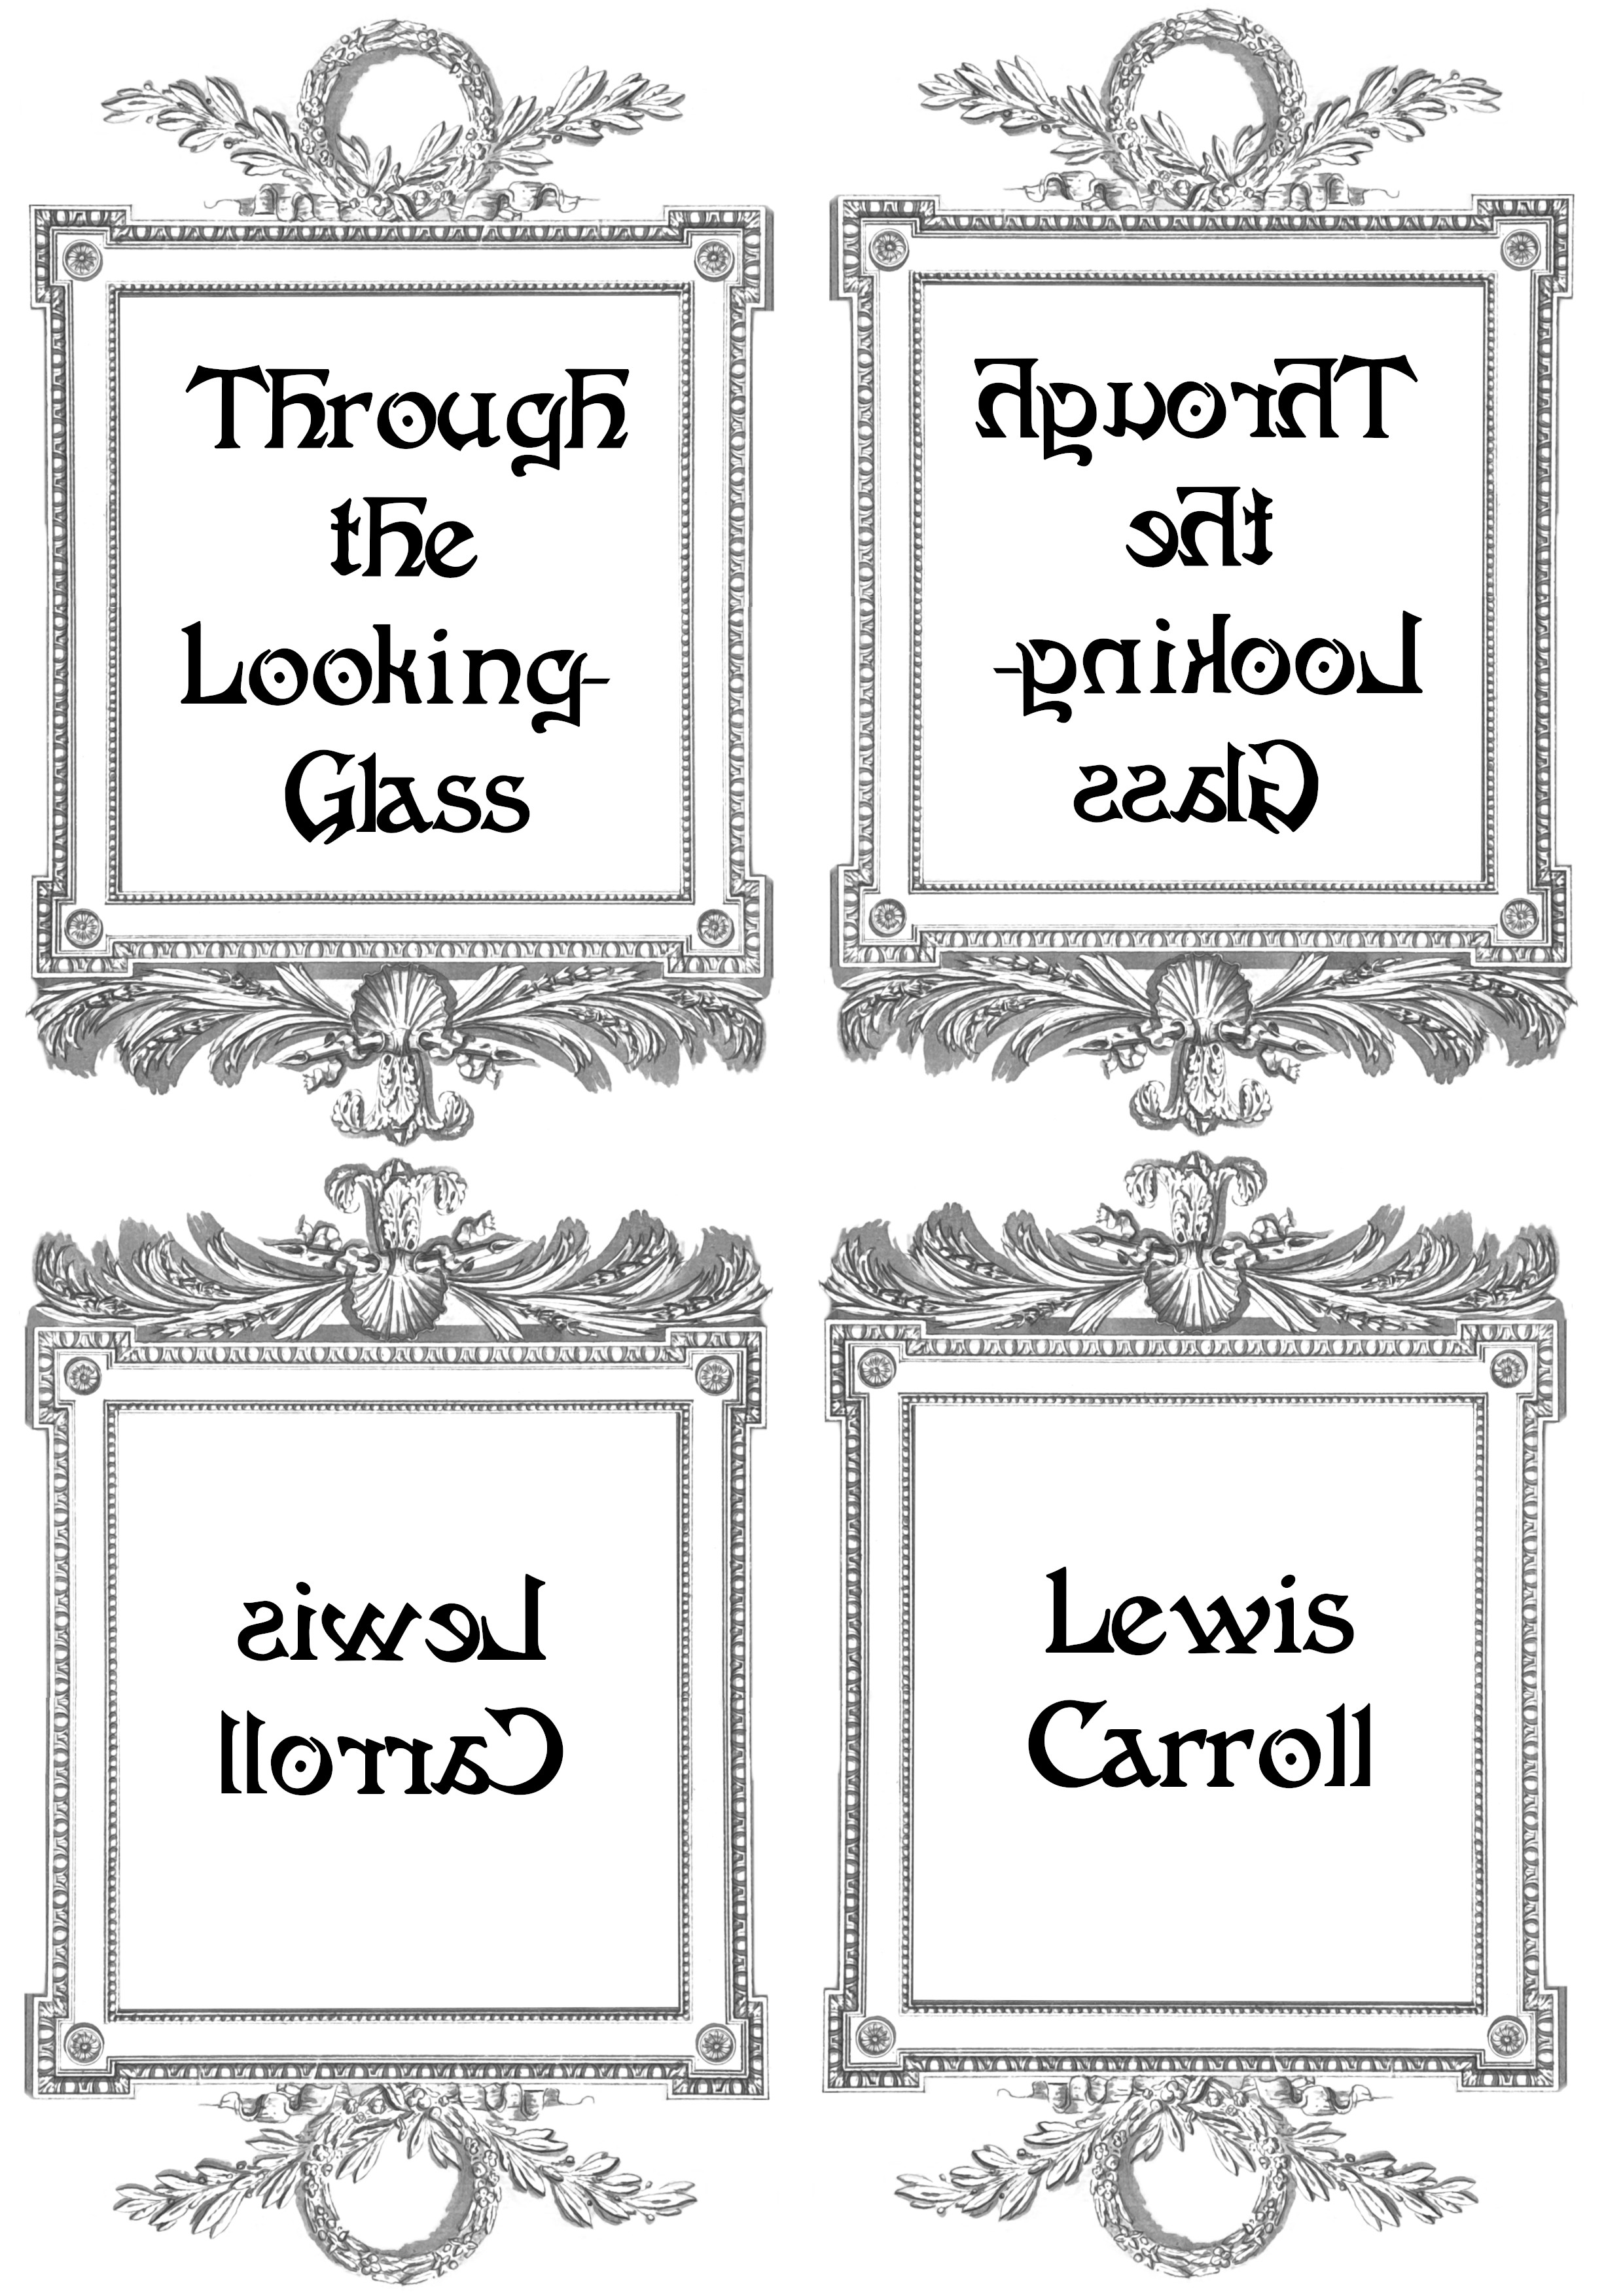
\includepdf[width=1.2\textwidth]{titlepage.jpg}
\clearpage
\end{pictures}


	\pagestyle{plain}

\tableofcontents



%\listoffigures
\KOMAoptions{headings=openleft}
\vspace*{\fill}
\begin{verse}
	\begin{altverse}
Child of the pure unclouded brow\\
And dreaming eyes of wonder!\\
Though time be fleet, and I and thou\\
Are half a life asunder,\\
Thy loving smile will surely hail\\
The love-gift of a fairy-tale.
\end{altverse}

	\begin{altverse}
I have not seen thy sunny face,\\
Nor heard thy silver laughter;\\
No thought of me shall find a place\\
In thy young life’s hereafter—\\
Enough that now thou wilt not fail\\
To listen to my fairy-tale.
\end{altverse}

	\begin{altverse}
A tale begun in other days,\\
When summer suns were glowing—\\
A simple chime, that served to time\\
The rhythm of oar rowing—\\
Whose echoes live in memory yet,\\
Though envious years would say »forget.«
\end{altverse}
\end{verse}
\vfill
\clearpage

\vspace*{\fill}
\begin{verse}
	\begin{altverse}
Come, hearken then, ere voice of dread.\\
With bitter tidings laden,\\
Shall summon to unwelcome bed\\
A melancholy maiden!\\
We are but older children, dear,\\
Who fret to find our bedtime near.
\end{altverse}

	\begin{altverse}
Without, the frost, the blinding snow.\\
The storm-wind’s moody madness—\\
Within, the firelight’s ruddy glow,\\
And childhood’s nest of gladness.\\
The magic words shall hold thee fast:\\
Thou shalt not heed the raving blast.
\end{altverse}

	\begin{altverse}
And though the shadow of a sigh\\
May tremble through the story,\\
For »happy summer days« gone by,\\
And vanish’d summer glory—\\
It shall not touch with breath of bale\\
The pleasance of our fairy-tale.
\end{altverse}
\end{verse}
\vfill

\chapter*{Dramatis Personæ}
	\pagestyle{plain}
\begin{center}
	\textit{(As arranged before commencement of game)}\\

\vfill
\begin{tabular}{c c c c}
\textsc{White pieces} & \textsc{White pawns} & \textsc{Red pawns} & \textsc{Red pieces}\\
  \hline
Tweedledee & Daisy & Daisy & Humpty Dumpty\\
Unicorn & Haigha & Messenger & Carpenter\\
Sheep & Oyster & Oyster & Walrus\\
W. Queen & »Lily« & Tiger-lily & R. Queen\\
W. King & Fawn & Rose & R. King\\
Aged man & Oyster & Oyster & Crow\\
W. Knight & Hatta & Frog & R. Knight\\
Tweedledum & Daisy & Daisy & Lion\\
\end{tabular}
\vfill
\textsc{red}\\
\vspace{-1em}
\chessboard[
    setpieces={Kc6,ng8,Nf5,ke4,qe2,Rf1,Pd2,Qc1},
    showmover=false,
]\\
\textsc{white}
\vfill
White Pawn (Alice) to play, and win in eleven moves




\end{center}

\begin{letter}
\clearpage
\vspace*{\fill}
\end{letter}

\begin{center}\Large\scshape
	Moves
\end{center}

\renewcommand{\arraystretch}{1.5} 

\begin{tabular}{l l r}
1. & Alice meets R.Q. & \pageref{white1}\\
\hspace{1em} 1. & \hspace{1em}R.Q. to K.R.'s 4th & \pageref{black1} \\
2. & Alice through Q.'s 3rd \textit{(by railway)} & \pageref{white2}\\
& to 4th \textit{(Tweedledum and Tweedledee)} & \pageref{white2b}\\
\hspace{1em} 2. & \hspace{1em}W.Q. to Q.B.'s 4th \textit{(after shawl)} & \pageref{black2}\\
3. & Alice meets W.Q. \textit{(with shawl)} & \pageref{white3}\\
\hspace{1em} 3. & \hspace{1em}W.Q. to Q.B.’s 5th \textit{(becomes sheep)} & \pageref{black3}\\
4. & Alice to Q.'s 5th \textit{(shop, river, shop)} & \pageref{white4}\\
\hspace{1em} 4. &  \hspace{1em}W.Q. to K.B.'s 8th \textit{(leaves egg on shelf)} & \pageref{black4}\\
5. & Alice to Q.'s 6th \textit{(Humpty Dumpty)} & \pageref{white5}\\
\hspace{1em} 5. &  \hspace{1em}W.Q. to Q.B's 8th \textit{(flying from R.Kt.)} & \pageref{black5}\\
6. & Alice to Q.'s 7th \textit{(forest)} & \pageref{white6}\\
\hspace{1em} 6. &  \hspace{1em}R.Kt. to K.'s 2nd \textit{(ch.)} & \pageref{black6}\\
7. & W.Kt. takes R.Kt. & \pageref{white7}\\
\hspace{1em} 7. &  \hspace{1em}W.Kt. to K.B.'s 5th & \pageref{black7}\\
8. & Alice to Q.'s 8th \textit{(coronation)} & \pageref{white8}\\
\hspace{1em} 8. &  \hspace{1em}R.Q. to K.'s sq \textit{(examination)} & \pageref{black8}\\
9. & Alice becomes Queen & \pageref{white9}\\
\hspace{1em} 9. &  \hspace{1em}Queen's castle & \pageref{black9}\\
10. & Alice castles \textit{(feast)} & \pageref{white10}\\
\hspace{1em} 10. &  \hspace{1em}W.Q. to Q.R. 6th \textit{(soup)} & \pageref{black10}\\
11. & Alice takes R.Q. and wins & \pageref{white11}\\
\end{tabular} 
\renewcommand{\arraystretch}{1} % reset the value to default

\vfill

\chapter*{Preface}

As the chess-problem, given on a previous page, has puzzled some of my readers, it may be well to explain that it is correctly worked out, so far as the \textit{moves} are concerned. The \textit{alternation} of Red and White is perhaps not so strictly observed as it might be, and the »castling« of the three Queens is merely a way of saying that they entered the palace; but the »check« of the White King at move 6, the capture of the Red Knight at move 7, and the final »check-mate« of the Red King, will be found, by any one who will take the trouble to set the pieces and play the moves as directed, to be strictly in accordance with the laws of the game.

The new words, in the poem »Jabberwocky« (see page \pageref{jabberwocky}), have given rise to some differences of opinion as to their pronunciation: so it may be well to give instructions on \textit{that} point also. Pronounce »slithy« as if it were to the words »sly, the«; make the »g« \textit{hard} in »gyre« and »gimble«; and pronounce »rath« to rhyme with »bath.«

~\\
~\\
Christmas, 1896
 
\mainmatter
\pagestyle{headings}
\KOMAoptions{headings=openright}
%!TeX root=../alicetop.tex



\chapter{Down the Rabbit-hole}
\lettrine[lines=4,findent=2pt]{A}{lice} was beginning to get very tired of sitting by her sister on the bank, and of having nothing to do: once or twice she had peeped into the book her sister was reading, but it had no pictures or conversations in it, »and what is the use of a book,« thought Alice, »without pictures or conversations?«

So she was considering in her own mind (as well as she could, for the hot day made her feel very sleepy and stupid) whether the pleasure of making a daisy-chain would be worth the trouble of getting up and picking the daisies, when suddenly a White Rabbit with pink eyes ran close by her.

There was nothing so \textit{very} remarkable in that; nor did Alice think it so \textit{very} much out of the way to hear the Rabbit say to itself, »Oh dear! Oh dear! I shall be too late!« (when she thought it over afterwards, it occurred to her that she ought to have wondered at this, but at the time it all seemed quite natural); but when the Rabbit actually \textit{took a watch out of its waistcoat-pocket}, and looked at it, and then hurried on, Alice started to her feet, for it flashed across her mind that she had never before seen a rabbit with either a waistcoat-pocket, or a watch to take out of it, and burning with curiosity, she ran across the field after it, and was just in time to see it pop down a large rabbit-hole under the hedge.

In another moment down went Alice after it, never once considering how in the world she was to get out again.

The rabbit-hole went straight on like a tunnel for some way, and then dipped suddenly down, so suddenly that Alice had not a moment to think about stopping herself before she found herself falling down what seemed to be a very deep well.

\begin{pictures}
	\begin{letter}
		
		\begin{figure}[t!]
		\centering
		\begin{tikzpicture}[remember picture, overlay,shift=(current page.north west)]
			\node (img) at ($(current page.center)+(0.2,-1.8cm)$) {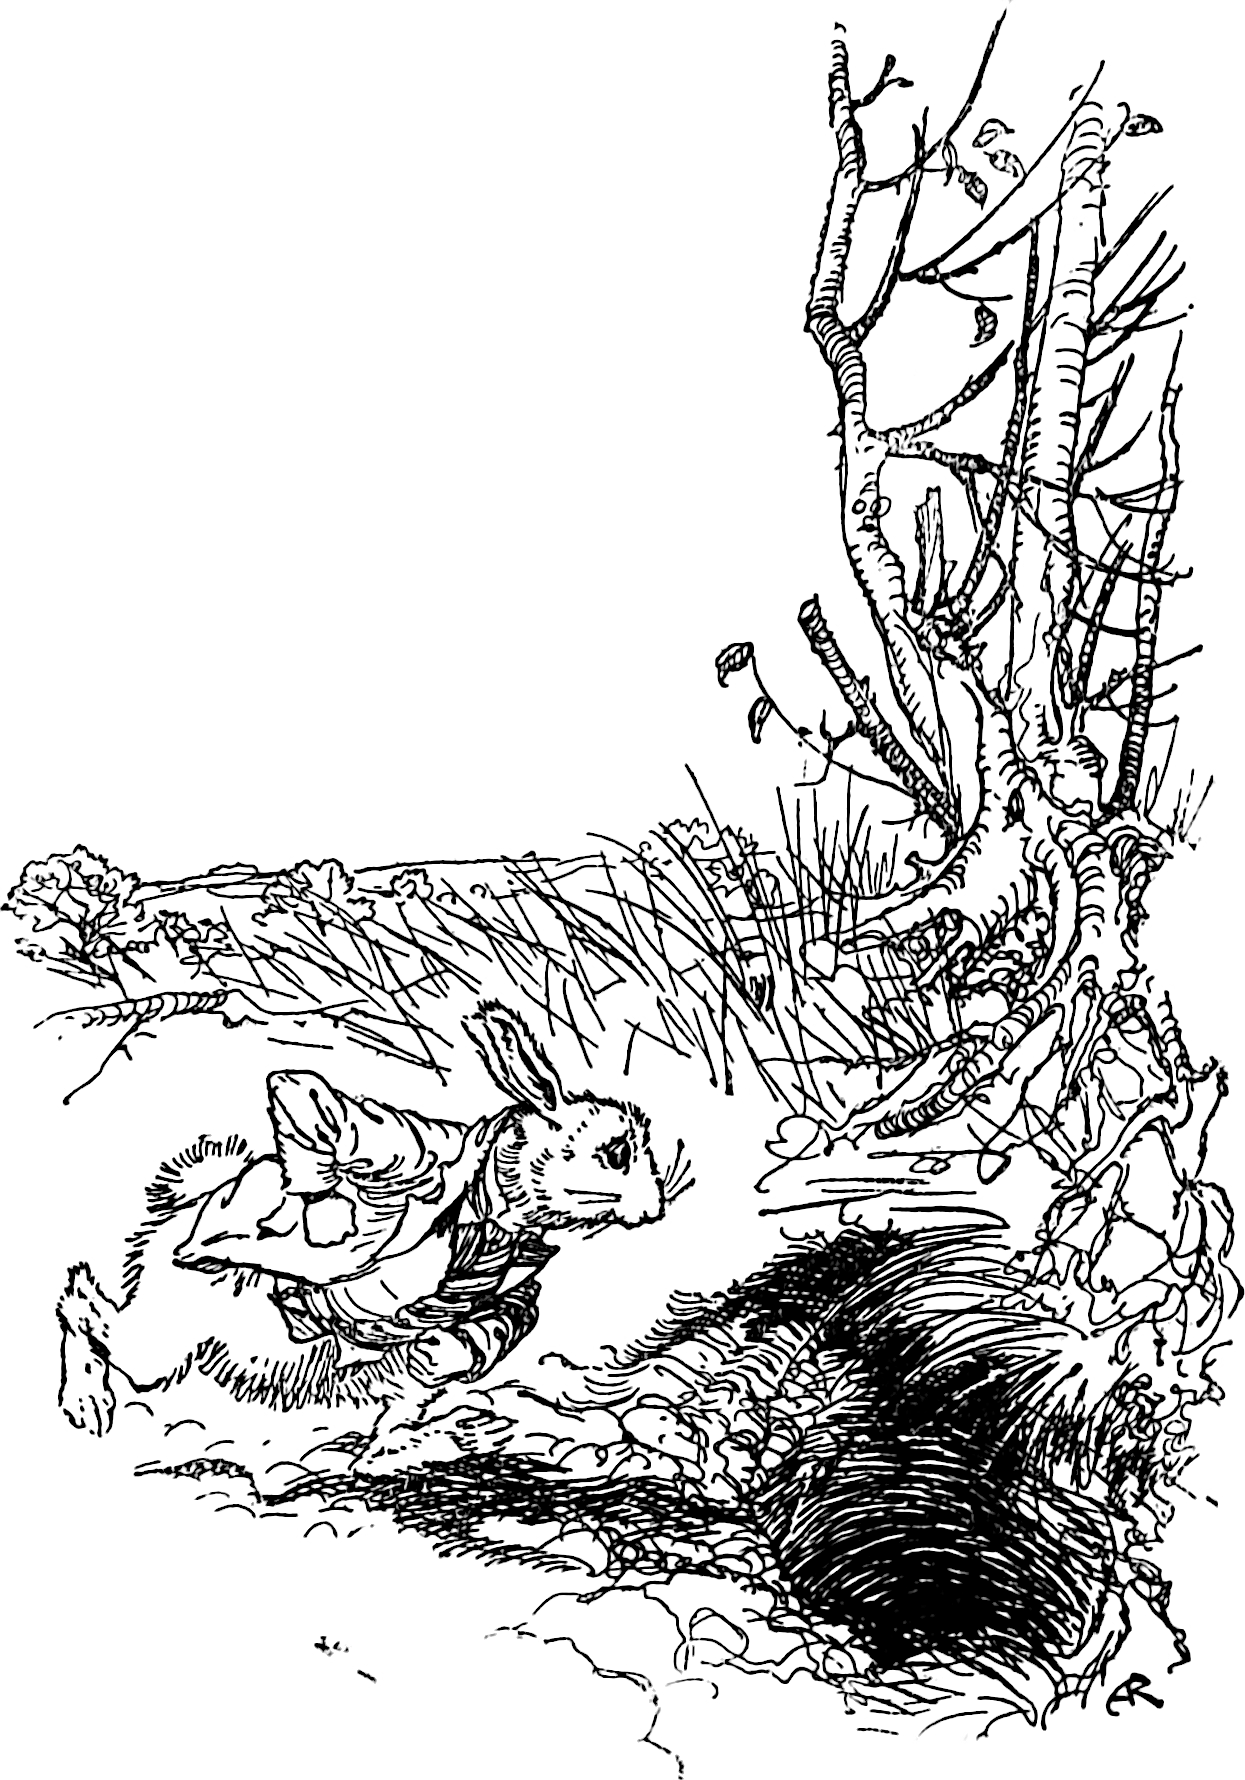
\includegraphics[width=1.1\textwidth]{imlate}};
			\node[text width=\textwidth,align=justify, anchor=north west, inner sep=0] (text1) at ($(current page.north west)+(1.7cm,-2.2cm)$) {
				\begin{minipage}{\textwidth}
				\parindent=1em
					Either the well was very deep, or she fell very slowly, for she had plenty of time as she went down to look about her, and to wonder what was going to happen next. First, she tried to look down and make out what she was coming to, but it was too dark to see anything; then she looked 
				\end{minipage}
			};

			\node[text width=\textwidth,align=justify, anchor=north west, inner sep=0, below=\lineskip+2pt of text1] (text2) {
				\begin{minipage}{0.64\textwidth}
				\parindent=1em

				\noindent at the sides of the well and noticed that they were filled with cupboards and book-shelves: here and there she saw maps and pictures hung upon pegs. She took down a jar from one of the shelves as she passed; it was labelled »\textsc{Orange Marmalade},« but to her disappointment it was empty; she did not like to drop the jar for fear of killing somebody underneath, so managed to put it into one of the cupboards as she fell past it.
					
						»Well!« thought Alice to herself. `After such a fall as this, I shall think nothing of tumbling
				\end{minipage}
			};
			\node[text width=\textwidth,align=justify, anchor=north west, inner sep=0, below=\lineskip+2pt of text2] (text3) {
				\begin{minipage}{0.55\textwidth}
	  down stairs! How brave they'll all think me at home! Why, I wouldn't say anything about it, even if I fell off the top of the house!' (Which was very likely true.)
				\end{minipage}
			};
		\end{tikzpicture}
	\end{figure}
	~ %quick'n'dirty hack to get the headers printing
	\end{letter}

	\begin{a4}
		
		\enlargethispage{\baselineskip}
		
		\begin{figure}[t!]
		\centering
		\begin{tikzpicture}[remember picture, overlay,shift=(current page.north west)]
			\node (img) at ($(current page.center)+(0.5cm,-1.5cm)$) {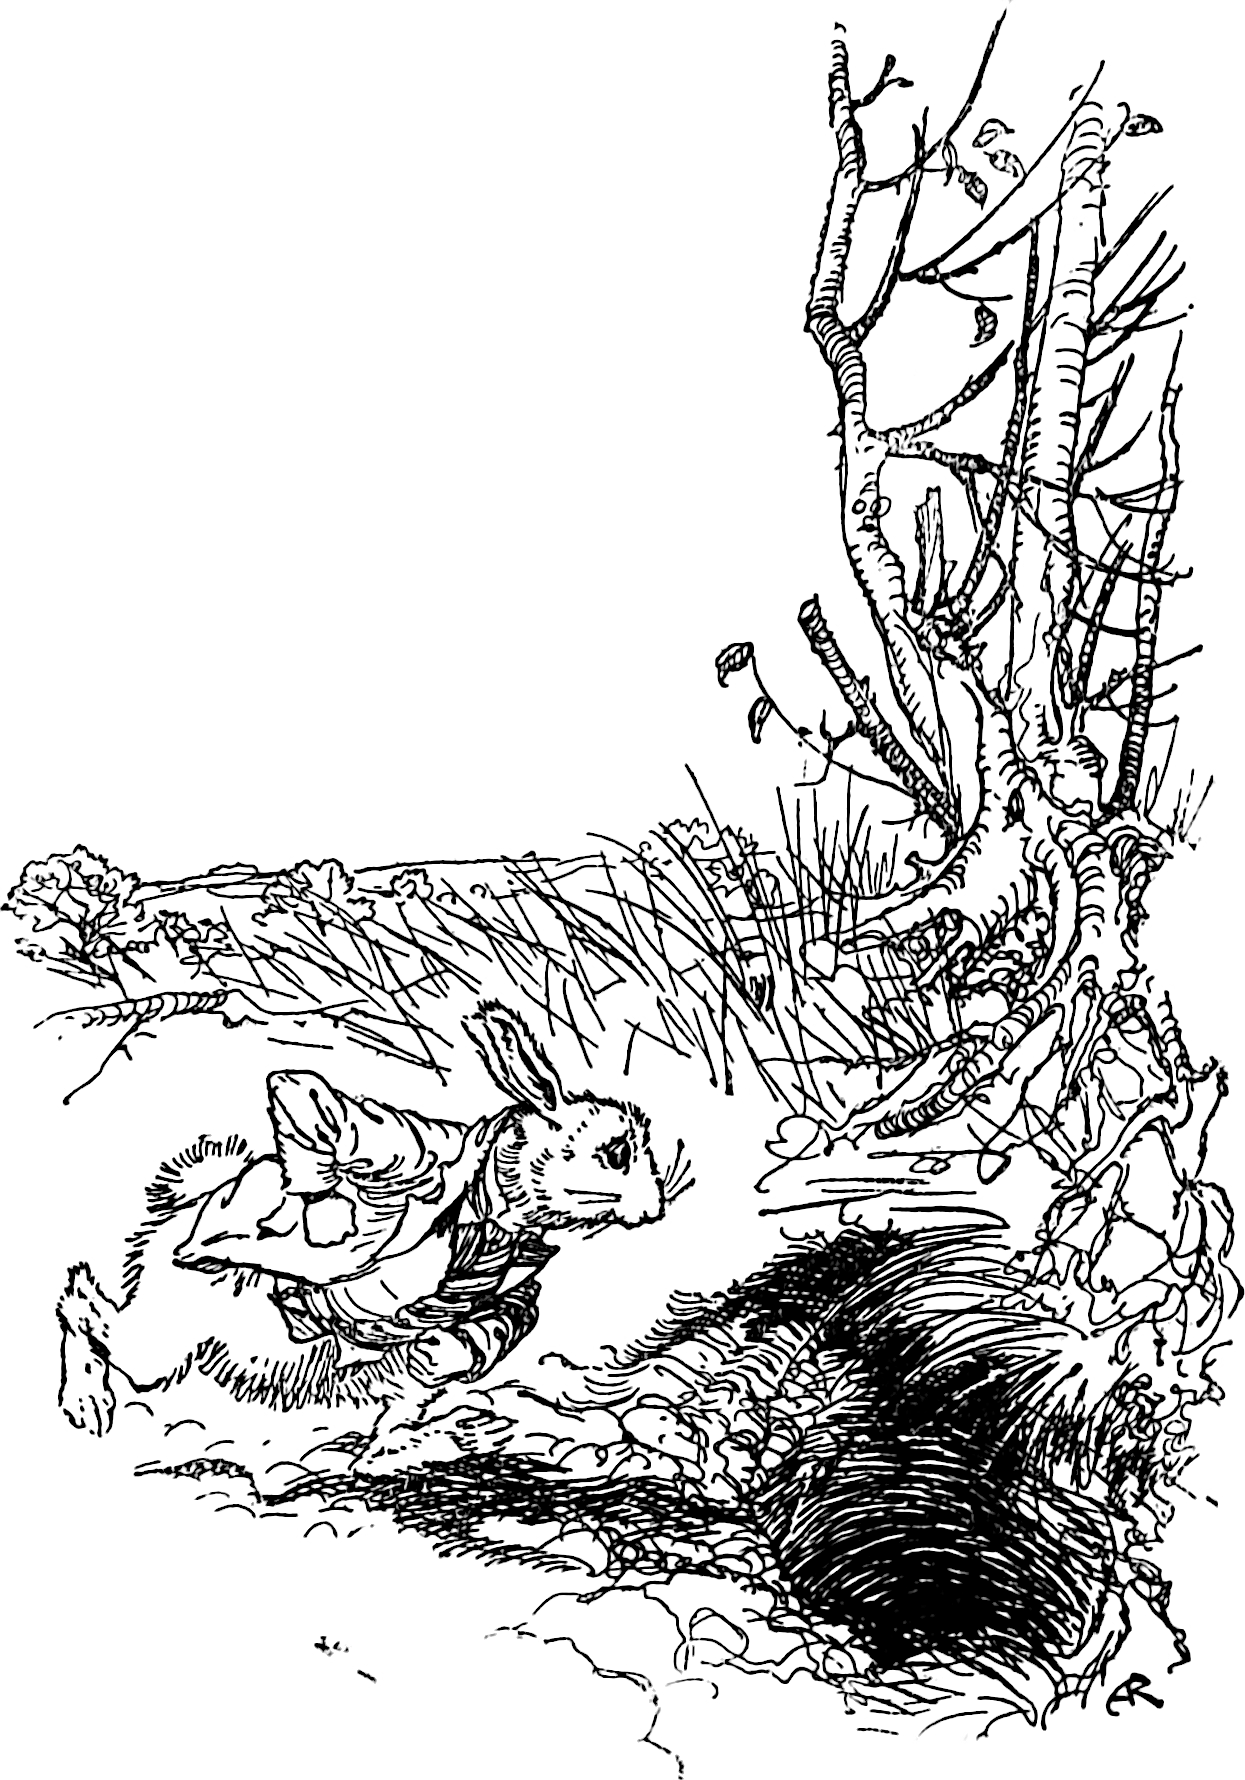
\includegraphics[width=\textwidth]{imlate}};
			\node[text width=\textwidth,align=justify, anchor=north west, inner sep=0] (text1) at ($(current page.north west)+(1.7cm,-2.4cm)$) {
				\begin{minipage}{\textwidth}
				\parindent=1em			
					Either the well was very deep, or she fell very slowly, for she had plenty of time as she went down to look about her, and to wonder what was going to happen next. First, she tried to look down and make out what she was coming to, but it was too dark to see anything; then she looked at the sides of the well
				\end{minipage}
			};

			\node[text width=\textwidth,align=justify, anchor=north west, inner sep=0, below=\lineskip+2pt of text1] (text2) {
				\begin{minipage}{0.68\textwidth}
				\parindent=1em

				\noindent and noticed that they were filled with cupboards and book-shelves: here and there she saw maps and pictures hung upon pegs. She took down a jar from one of the shelves as she passed; it was labelled »\textsc{Orange Marmalade},« but to her disappointment it was empty; she did not like to drop the jar for fear of killing somebody underneath, so managed to put it into one of the cupboards as she fell past it.
					
						»Well!« thought Alice to herself. `After such a fall as this, I shall think nothing of tumbling down stairs!
				\end{minipage}
			};
			\node[text width=\textwidth,align=justify, anchor=north west, inner sep=0, below=\lineskip of text2] (text3) {
				\begin{minipage}{0.6\textwidth}
	   How brave they'll all think me at home! Why, I wouldn't say anything about it, even if I fell off the top of the house!' (Which was very likely true.)
				\end{minipage}
			};
		\end{tikzpicture}
	\end{figure}
	\end{a4}
	~ %quick'n'dirty hack to get the headers printing

	\clearpage
\end{pictures}

\begin{placeholder}
Either the well was very deep, or she fell very slowly, for she had plenty of time as she went down to look about her, and to wonder what was going to happen next. First, she tried to look down and make out what she was coming to, but it was too dark to see anything; then she looked at the sides of the well and noticed that they were filled with cupboards and book-shelves: here and there she saw maps and pictures hung upon pegs. She took down a jar from one of the shelves as she passed; it was labelled »\textsc{Orange Marmalade},« but to her disappointment it was empty; she did not like to drop the jar for fear of killing somebody underneath, so managed to put it into one of the cupboards as she fell past it.

»Well!« thought Alice to herself. »After such a fall as this, I shall think nothing of tumbling down stairs! How brave they'll all think me at home! Why, I wouldn't say anything about it, even if I fell off the top of the house!« (Which was very likely true.)
\clearpage
\end{placeholder}

Down, down, down. Would the fall \textit{never} come to an end? »I wonder how many miles I've fallen by this time?« she said aloud. »I must be getting somewhere near the centre of the earth. Let me see: that would be four thousand miles down. I think\longdash« (for, you see, Alice had learnt several things of this sort in her lessons in the schoolroom, and though this was not a \textit{very} good opportunity for showing off her knowledge, as there was no one to listen to her, still it was good practice to say it over) »—yes, that's about the right distance—but then I wonder what Latitude or Longitude I've got to?« (Alice had no idea what Latitude was, or Longitude either, but thought they were nice grand words to say.)

Presently she began again. »I wonder if I shall fall right \textit{through} the earth! How funny it'll seem to come out among the people that walk with their heads downwards! The Antipathies, I think\longdash« (she was rather glad there \textit{was} no one listening, this time, as it didn't sound at all the right word) »—but I shall have to ask them what the name of the country is, you know. Please, Ma'am, is this New Zealand or Australia?« (and she tried to curtsey as she spoke—fancy \textit{curtseying} as you're falling through the air! Do you think you could manage it?) »And what an ignorant little girl she'll think me! No, it'll never do to ask: perhaps I shall see it written up somewhere.«



 
 
Down, down, down. There was nothing else to do, so Alice soon began talking again. »Dinah'll miss me very much to-night, I should think!« (Dinah was the cat.) »I hope they'll remember her saucer of milk at tea-time. Dinah, my dear, I wish you were down here with me! There are no mice in the air, I'm afraid, but you might catch a bat, and that's very like a mouse, you know. But do cats eat bats, I wonder?« And here Alice began to get rather sleepy, and went on saying to herself, in a dreamy sort of way, »Do cats eat bats? Do cats eat bats?« and sometimes, »Do bats eat cats?« for, you see, as she couldn't answer either question, it didn't much matter which way she put it. She felt that she was dozing off, and had just begun to dream that she was walking hand in hand with Dinah, and saying to her very earnestly, »Now, Dinah, tell me the truth: did you ever eat a bat?« when suddenly, thump! thump! down she came upon a heap of sticks and dry leaves, and the fall was over.

Alice was not a bit hurt, and she jumped up on to her feet in a moment: she looked up, but it was all dark overhead; before her was another long passage, and the White Rabbit was still in sight, hurrying down it. There was not a moment to be lost: away went Alice like the wind, and was just in time to hear it say, as it turned a corner, »Oh my ears and whiskers, how late it's getting!« She was close behind it when she turned the corner, but the Rabbit was no longer to be seen: she found herself in a long, low hall, which was lit up by a row of lamps hanging from the roof.

There were doors all round the hall, but they were all locked; and when Alice had been all the way down one side and up the other, trying every door, she walked sadly down the middle, wondering how she was ever to get out again.

Suddenly she came upon a little three-legged table, all made of solid glass; there was nothing on it but a tiny golden key, and Alice's first idea was that this might belong to one of the doors of the hall; but, alas! either the locks were too large, or the key was too small, but at any rate it would not open any of them. However, on the second time round, she came upon a low curtain she had not noticed before, and behind it was a little door about fifteen inches high: she tried the little golden key in the lock, and to her great delight it fitted!

Alice opened the door and found that it led into a small passage, not much larger than a rat-hole: she knelt down and looked along the passage into the loveliest garden you ever saw. How she longed to get out of that dark hall, and wander about among those beds of bright flowers and those cool fountains, but she could not even get her head through the doorway; »even if my head would go through,« thought poor Alice, »it would be of very little use without my shoulders. Oh, how I wish I could shut up like a telescope! I think I could, if I only knew how to begin.« For, you see, so many out-of-the-way things had happened lately, that Alice had begun to think that very few things indeed were really impossible.

There seemed to be no use in waiting by the little door, so she went back to the table, half hoping she might find another key on it, or at any rate a book of rules for shutting people up like telescopes: this time she found a little bottle on it (»which certainly was not here before,« said Alice,) and tied round the neck of the bottle was a paper label, with the words »\textsc{drink me}« beautifully printed on it in large letters.

It was all very well to say »Drink me,« but the wise little Alice was not going to do \textit{that} in a hurry. »No, I'll look first,« she said, »and see whether it's marked »\textit{poison}« or not;« for she had read several nice little stories about children who had got burnt, and eaten up by wild beasts, and other unpleasant things, all because they \textit{would} not remember the simple rules their friends had taught them: such as, that a red-hot poker will burn you if you hold it too long; and that, if you cut your finger \textit{very} deeply with a knife, it usually bleeds; and she had never forgotten that, if you drink much from a bottle marked »poison,« it is almost certain to disagree with you, sooner or later.

However, this bottle was \textit{not} marked »poison,« so Alice ventured to taste it, and finding it very nice (it had, in fact, a sort of mixed flavour of cherry-tart, custard, pineapple, roast turkey, coffee, and hot buttered toast,) she very soon finished it off.

\divider

»What a curious feeling!« said Alice. »I must be shutting up like a telescope.«

And so it was indeed: she was now only ten inches high, and her face brightened up at the thought that she was now the right size for going through that little door into that lovely garden. First, however, she waited for a few minutes to see if she was going to shrink any further: she felt a little nervous about this: »for it might end, you know,« said Alice to herself, »in my going out altogether, like a candle. I wonder what I should be like then?« And she tried to fancy what the flame of a candle looks like after the candle is blown out, for she could not remember ever having seen such a thing.

After a while, finding that nothing more happened, she decided on going into the garden at once; but, alas for poor Alice! when she got to the door, she found she had forgotten the little golden key, and when she went back to the table for it, she found she could not possibly reach it: she could see it quite plainly through the glass, and she tried her best to climb up one of the legs of the table, but it was too slippery; and when she had tired herself out with trying, the poor little thing sat down and cried.

»Come, there's no use in crying like that!« said Alice to herself, rather sharply. »I advise you to leave off this minute!« She generally gave herself very good advice (though she very seldom followed it), and sometimes she scolded herself so severely as to bring tears into her eyes; and once she remembered trying to box her own ears for having cheated herself in a game of croquet she was playing against herself, for this curious child was very fond of pretending to be two people. »But it's no use now,« thought poor Alice, »to pretend to be two people! Why there's hardly enough of me left to make \textit{one} respectable person!«

Soon her eye fell on a little glass box that was lying under the table: she opened it, and found in it a very small cake, on which the words »\textsc{eat me}« were beautifully marked in currants. »Well, I'll eat it,« said Alice, »and if it makes me grow larger, I can reach the key; and if it makes me grow smaller, I can creep under the door; so either way I'll get into the garden, and I don't care which happens!«

She ate a little bit, and said anxiously to herself, »Which way? Which way?« holding her hand on the top of her head to feel which way it was growing, and she was quite surprised to find that she remained the same size; to be sure, this is what generally happens when one eats cake, but Alice had got so much into the way of expecting nothing but out-of-the-way things to happen, that it seemed quite dull and stupid for life to go on in the common way.

So she set to work, and very soon finished off the cake.
%!TeX root=../glasstop.tex
\chapter{The Garden of Live Flowers}

\lettrine[lines=4,ante=`]{I}{} should see the garden far better,' said Alice to herself, »if I could get to the top of that hill: and here's a path that leads straight to it—at least, no, it doesn't do that\longdash« (after going a few yards along the path, and turning several sharp corners), »but I suppose it will at last. But how curiously it twists! It's more like a corkscrew than a path! Well, \textit{this} turn goes to the hill, I suppose—no, it doesn't! This goes straight back to the house! Well then, I'll try it the other way.«

And so she did: wandering up and down, and trying turn after turn, but always coming back to the house, do what she would. Indeed, once, when she turned a corner rather more quickly than usual, she ran against it before she could stop herself.

»It's no use talking about it,« Alice said, looking up at the house and pretending it was arguing with her. »I'm \textit{not} going in again yet. I know I should have to get through the Looking-glass again—back into the old room—and there'd be an end of all my adventures!«

So, resolutely turning her back upon the house, she set out once more down the path, determined to keep straight on till she got to the hill. For a few minutes all went on well, and she was just saying, »I really \textit{shall} do it this time\longdash« when the path gave a sudden twist and shook itself (as she described it afterwards), and the next moment she found herself actually walking in at the door.

»Oh, it's too bad!« she cried. »I never saw such a house for getting in the way! Never!«

However, there was the hill full in sight, so there was nothing to be done but start again. This time she came upon a large flower-bed, with a border of daisies, and a willow-tree growing in the middle.

»O Tiger-lily,« said Alice, addressing herself to one that was waving gracefully about in the wind, »I \textit{wish} you could talk!«

»We \textit{can} talk,« said the Tiger-lily: »when there's anybody worth talking to.«

Alice was so astonished that she could not speak for a minute: it quite seemed to take her breath away. At length, as the Tiger-lily only went on waving about, she spoke again, in a timid voice—almost in a whisper. »And can \textit{all} the flowers talk?«

»As well as \textit{you} can,« said the Tiger-lily. »And a great deal louder.«

»It isn't manners for us to begin, you know,« said the Rose, »and I really was wondering when you'd speak! Said I to myself, »Her face has got \textit{some} sense in it, though it's not a clever one!« Still, you're the right colour, and that goes a long way.«

»I don't care about the colour,« the Tiger-lily remarked. »If only her petals curled up a little more, she'd be all right.«

Alice didn't like being criticised, so she began asking questions. »Aren't you sometimes frightened at being planted out here, with nobody to take care of you?«

»There's the tree in the middle,« said the Rose: »what else is it good for?«

»But what could it do, if any danger came?« Alice asked.

»It says »Bough-wough!«« cried a Daisy: »that's why its branches are called boughs!«

»Didn't you know \textit{that?}« cried another Daisy, and here they all began shouting together, till the air seemed quite full of little shrill voices. »Silence, every one of you!« cried the Tiger-lily, waving itself passionately from side to side, and trembling with excitement. »They know I can't get at them!« it panted, bending its quivering head towards Alice, »or they wouldn't dare to do it!«

»Never mind!« Alice said in a soothing tone, and stooping down to the daisies, who were just beginning again, she whispered, »If you don't hold your tongues, I'll pick you!«

There was silence in a moment, and several of the pink daisies turned white.

»That's right!« said the Tiger-lily. »The daisies are worst of all. When one speaks, they all begin together, and it's enough to make one wither to hear the way they go on!«

»How is it you can all talk so nicely?« Alice said, hoping to get it into a better temper by a compliment. »I've been in many gardens before, but none of the flowers could talk.«

»Put your hand down, and feel the ground,« said the Tiger-lily. »Then you'll know why.«

Alice did so. »It's very hard,« she said, »but I don't see what that has to do with it.«

»In most gardens,« the Tiger-lily said, »they make the beds too soft—so that the flowers are always asleep.«

This sounded a very good reason, and Alice was quite pleased to know it. »I never thought of that before!« she said.

»It's \textit{my} opinion that you never think \textit{at all,}« the Rose said in a rather severe tone.

»I never saw anybody that looked stupider,« a Violet said, so suddenly, that Alice quite jumped; for it hadn't spoken before.

»Hold \textit{your} tongue!« cried the Tiger-lily. »As if \textit{you} ever saw anybody! You keep your head under the leaves, and snore away there, till you know no more what's going on in the world, than if you were a bud!«

»Are there any more people in the garden besides me?« Alice said, not choosing to notice the Rose's last remark.

»There's one other flower in the garden that can move about like you,« said the Rose. »I wonder how you do it\longdash« (»You're always wondering,« said the Tiger-lily), »but she's more bushy than you are.«

»Is she like me?« Alice asked eagerly, for the thought crossed her mind, »There's another little girl in the garden, somewhere!«

»Well, she has the same awkward shape as you,« the Rose said, »but she's redder—and her petals are shorter, I think.«

»Her petals are done up close, almost like a dahlia,« the Tiger-lily interrupted: »not tumbled about anyhow, like yours.«

»But that's not \textit{your} fault,« the Rose added kindly: »you're beginning to fade, you know—and then one can't help one's petals getting a little untidy.«

Alice didn't like this idea at all: so, to change the subject, she asked »Does she ever come out here?«

»I daresay you'll see her soon,« said the Rose. »She's one of the thorny kind.«

»Where does she wear the thorns?« Alice asked with some curiosity.

»Why all round her head, of course,« the Rose replied. »I was wondering \textit{you} hadn't got some too. I thought it was the regular rule.«

»She's coming!« cried the Larkspur. »I hear her footstep, thump, thump, thump, along the gravel-walk!«


Alice looked round eagerly, and found that it was the Red Queen. \label{white1} »She's grown a good deal!« was her first remark. She had indeed: when Alice first found her in the ashes, she had been only three inches high—and here she was, half a head taller than Alice herself!

»It's the fresh air that does it,« said the Rose: »wonderfully fine air it is, out here.«

»I think I'll go and meet her,« said Alice, for, though the flowers were interesting enough, she felt that it would be far grander to have a talk with a real Queen.

»You can't possibly do that,« said the Rose: »\textit{I} should advise you to walk the other way.«

This sounded nonsense to Alice, so she said nothing, but set off at once towards the Red Queen. To her surprise, she lost sight of her in a moment, and found herself walking in at the front-door again.

A little provoked, she drew back, and after looking everywhere for the queen (whom she spied out at last, a long way off), she thought she would try the plan, this time, of walking in the opposite direction.

It succeeded beautifully. She had not been walking a minute before she found herself face to face with the Red Queen, and full in sight of the hill she had been so long aiming at.

»Where do you come from?« said the Red Queen. »And where are you going? Look up, speak nicely, and don't twiddle your fingers all the time.«

Alice attended to all these directions, and explained, as well as she could, that she had lost her way.

»I don't know what you mean by \textit{your} way,« said the Queen: »all the ways about here belong to \textit{me}—but why did you come out here at all?« she added in a kinder tone. »Curtsey while you're thinking what to say, it saves time.«

Alice wondered a little at this, but she was too much in awe of the Queen to disbelieve it. »I'll try it when I go home,« she thought to herself, »the next time I'm a little late for dinner.«

»It's time for you to answer now,« the Queen said, looking at her watch: »open your mouth a \textit{little} wider when you speak, and always say »your Majesty.««

»I only wanted to see what the garden was like, your Majesty\longdash«

»That's right,« said the Queen, patting her on the head, which Alice didn't like at all, »though, when you say »garden,«—\textit{I've} seen gardens, compared with which this would be a wilderness.«

Alice didn't dare to argue the point, but went on: »—and I thought I'd try and find my way to the top of that hill\longdash«

»When you say »hill,«« the Queen interrupted, »\textit{I} could show you hills, in comparison with which you'd call that a valley.«

»No, I shouldn't,« said Alice, surprised into contradicting her at last: »a hill \textit{can't} be a valley, you know. That would be nonsense\longdash«

The Red Queen shook her head, »You may call it »nonsense« if you like,« she said, »but \textit{I've} heard nonsense, compared with which that would be as sensible as a dictionary!«

Alice curtseyed again, as she was afraid from the Queen's tone that she was a \textit{little} offended: and they walked on in silence till they got to the top of the little hill.

For some minutes Alice stood without speaking, looking out in all directions over the country—and a most curious country it was. There were a number of tiny little brooks running straight across it from side to side, and the ground between was divided up into squares by a number of little green hedges, that reached from brook to brook.

»I declare it's marked out just like a large chessboard!« Alice said at last. »There ought to be some men moving about somewhere—and so there are!« She added in a tone of delight, and her heart began to beat quick with excitement as she went on. »It's a great huge game of chess that's being played—all over the world—if this \textit{is} the world at all, you know. Oh, what fun it is! How I \textit{wish} I was one of them! I wouldn't mind being a Pawn, if only I might join—though of course I should \textit{like} to be a Queen, best.«

She glanced rather shyly at the real Queen as she said this, but her companion only smiled pleasantly, and said, »That's easily managed. You can be the White Queen's Pawn, if you like, as Lily's too young to play; and you're in the Second Square to begin with: when you get to the Eighth Square you'll be a Queen\longdash« Just at this moment, somehow or other, they began to run.

Alice never could quite make out, in thinking it over afterwards, how it was that they began: all she remembers is, that they were running hand in hand, and the Queen went so fast that it was all she could do to keep up with her: and still the Queen kept crying »Faster! Faster!« but Alice felt she \textit{could not} go faster, though she had not breath left to say so.

The most curious part of the thing was, that the trees and the other things round them never changed their places at all: however fast they went, they never seemed to pass anything. »I wonder if all the things move along with us?« thought poor puzzled Alice. And the Queen seemed to guess her thoughts, for she cried, »Faster! Don't try to talk!«

Not that Alice had any idea of doing \textit{that}. She felt as if she would never be able to talk again, she was getting so much out of breath: and still the Queen cried »Faster! Faster!« and dragged her along. »Are we nearly there?« Alice managed to pant out at last.

»Nearly there!« the Queen repeated. »Why, we passed it ten minutes ago! Faster!« And they ran on for a time in silence, with the wind whistling in Alice's ears, and almost blowing her hair off her head, she fancied.

»Now! Now!« cried the Queen. »Faster! Faster!« And they went so fast that at last they seemed to skim through the air, hardly touching the ground with their feet, till suddenly, just as Alice was getting quite exhausted, they stopped, and she found herself sitting on the ground, breathless and giddy.

\label{black1}
The Queen propped her up against a tree, and said kindly, »You may rest a little now.«

Alice looked round her in great surprise. »Why, I do believe we've been under this tree the whole time! Everything's just as it was!«

»Of course it is,« said the Queen, »what would you have it?«

»Well, in \textit{our} country,« said Alice, still panting a little, »you'd generally get to somewhere else—if you ran very fast for a long time, as we've been doing.«

»A slow sort of country!« said the Queen. »Now, \textit{here,} you see, it takes all the running \textit{you} can do, to keep in the same place. If you want to get somewhere else, you must run at least twice as fast as that!«

»I'd rather not try, please!« said Alice. »I'm quite content to stay here—only I \textit{am} so hot and thirsty!«

»I know what \textit{you'd} like!« the Queen said good-naturedly, taking a little box out of her pocket. »Have a biscuit?«

Alice thought it would not be civil to say »No,« though it wasn't at all what she wanted. So she took it, and ate it as well as she could: and it was \textit{very} dry; and she thought she had never been so nearly choked in all her life.

»While you're refreshing yourself,« said the Queen, »I'll just take the measurements.« And she took a ribbon out of her pocket, marked in inches, and began measuring the ground, and sticking little pegs in here and there.

»At the end of two yards,« she said, putting in a peg to mark the distance, »I shall give you your directions—have another biscuit?«

»No, thank you,« said Alice: »one's \textit{quite} enough!«

»Thirst quenched, I hope?« said the Queen.

Alice did not know what to say to this, but luckily the Queen did not wait for an answer, but went on. »At the end of \textit{three} yards I shall repeat them—for fear of your forgetting them. At the end of \textit{four,} I shall say good-bye. And at the end of \textit{five,} I shall go!«

She had got all the pegs put in by this time, and Alice looked on with great interest as she returned to the tree, and then began slowly walking down the row.

At the two-yard peg she faced round, and said, »A pawn goes two squares in its first move, you know. So you'll go \textit{very} quickly through the Third Square—by railway, I should think—and you'll find yourself in the Fourth Square in no time. Well, \textit{that} square belongs to Tweedledum and Tweedledee—the Fifth is mostly water—the Sixth belongs to Humpty Dumpty—But you make no remark?«

»I—I didn't know I had to make one—just then,« Alice faltered out.

»You \textit{should} have said, »It's extremely kind of you to tell me all this«—however, we'll suppose it said—the Seventh Square is all forest—however, one of the Knights will show you the way—and in the Eighth Square we shall be Queens together, and it's all feasting and fun!« Alice got up and curtseyed, and sat down again.

At the next peg the Queen turned again, and this time she said, »Speak in French when you can't think of the English for a thing—turn out your toes as you walk—and remember who you are!« She did not wait for Alice to curtsey this time, but walked on quickly to the next peg, where she turned for a moment to say »good-bye,« and then hurried on to the last.

How it happened, Alice never knew, but exactly as she came to the last peg, she was gone. Whether she vanished into the air, or whether she ran quickly into the wood (»and she \textit{can} run very fast!« thought Alice), there was no way of guessing, but she was gone, and Alice began to remember that she was a Pawn, and that it would soon be time for her to move.
%!TeX root=../alicetop.tex
\chapter{A Caucus-race and a Long Tale}
	
\lettrine[lines=4,findent=2pt]{T}{hey} were indeed a queer-looking party that assembled on the bank—the birds with draggled feathers, the animals with their fur clinging close to them, and all dripping wet, cross, and uncomfortable.
	
The first question of course was, how to get dry again: they had a consultation about this, and after a few minutes it seemed quite natural to Alice to find herself talking familiarly with them, as if she had known them all her life. Indeed, she had quite a long argument with the Lory, who at last turned sulky, and would only say, »I am older than you, and must know better;« and this Alice would not allow without knowing how old it was, and, as the Lory positively refused to tell its age, there was no more to be said.

At last the Mouse, who seemed to be a person of authority among them, called out »Sit down, all of you, and listen to me! \textit{I'll} soon make you dry enough!« They all sat down at once, in a large ring, with the Mouse in the middle. Alice kept her eyes anxiously fixed on it, for she felt sure she would catch a bad cold if she did not get dry very soon.

»Ahem!« said the Mouse with an important air. »Are you all ready? This is the driest thing I know. Silence all round, if you please! »William the Conqueror, whose cause was favoured by the pope, was soon submitted to by the English, who wanted leaders, and had been of late much accustomed to usurpation and conquest. Edwin and Morcar, the earls of Mercia and Northumbria\longdash««

»Ugh!« said the Lory, with a shiver.

»I beg your pardon!« said the Mouse, frowning, but very politely. »Did you speak?«

»Not I\@!« said the Lory hastily.

»I thought you did,« said the Mouse, »—I proceed. »Edwin and Morcar, the earls of Mercia and Northumbria, declared for him: and even Stigand, the patriotic Archbishop of Canterbury, found it advisable\longdash««

»Found \textit{what?}« said the Duck.

»Found \textit{it,}« the Mouse replied rather crossly: »of course you know what »it« means.«

»I know what »it« means well enough, when \textit{I} find a thing,« said the Duck; »it's generally a frog or a worm. The question is, what did the archbishop find?«

The Mouse did not notice this question, but hurriedly went on, »»—found it advisable to go with Edgar Atheling to meet William and offer him the crown. William's conduct at first was moderate. But the insolence of his Normans\longdash« How are you getting on now, my dear?« it continued, turning to Alice as it spoke.

»As wet as ever,« said Alice in a melancholy tone; »doesn't seem to dry me at all.«

»In that case,« said the Dodo solemnly, rising to its feet, »I move that the meeting adjourn, for the immediate adoption of more energetic remedies\longdash«

»Speak English!« said the Eaglet. »I don't know the meaning of half those long words, and, what's more, I don't believe you do either!« And the Eaglet bent down its head to hide a smile: some of the other birds tittered audibly.

»What I was going to say,« said the Dodo in an offended tone, »was that the best thing to get us dry would be a Caucus-race.«

\begin{pictures}
	\begin{letter}
		\begin{colorbigpic}
			[1.1]
			{whohaswon}
			{They all crowded round it panting and asking, »But who has won?«}
		\end{colorbigpic}
	\end{letter}
	
	\begin{a4}
		\begin{colorbigpic}
			[1.0]
			{whohaswon}
			{They all crowded round it panting and asking, »But who has won?«}
		\end{colorbigpic}
	\end{a4}	
\end{pictures}


»What \textit{is} a Caucus-race?« said Alice; not that she much wanted to know, but the Dodo had paused as if it thought that \textit{somebody} ought to speak, and no one else seemed inclined to say anything.

»Why,« said the Dodo, »the best way to explain it is to do it.« (And, as you might like to try the thing yourself some winter day, I will tell you how the Dodo managed it.)

First it marked out a race-course, in a sort of circle, (»the exact shape doesn't matter,« it said,) and then all the party were placed along the course, here and there. There was no »One, two, three, and away,« but they began running when they liked, and left off when they liked, so that it was not easy to know when the race was over. However, when they had been running half an hour or so, and were quite dry again, the Dodo suddenly called »The race is over!« and they all crowded round it, panting, and asking »But who has won?«



This question the Dodo could not answer without a great deal of thought, and it stood for a long time with one finger pressed upon its forehead (the position in which you usually see Shakespeare, in the pictures of him), while the rest waited in silence. At last the Dodo said »\textit{Everybody} has won, and \textit{all} must have prizes.«

»But who is to give the prizes?« quite a chorus of voices asked.

»Why, \textit{she}, of course,« said the Dodo, pointing to Alice with one finger; and the whole party at once crowded round her, calling out in a confused way, »Prizes! Prizes!«

Alice had no idea what to do, and in despair she put her hand in her pocket, and pulled out a box of comfits (luckily the salt water had not got into it), and handed them round as prizes. There was exactly one apiece all round.

They all crowded round it panting and asking, »But who has won?«


»But she must have a prize herself, you know,« said the Mouse.

»Of course,« the Dodo replied very gravely.

»What else have you got in your pocket?« it went on, turning to Alice.

»Only a thimble,« said Alice sadly.

»Hand it over here,« said the Dodo.

Then they all crowded round her once more, while the Dodo solemnly presented the thimble, saying »We beg your acceptance of this elegant thimble;« and, when it had finished this short speech, they all cheered.

Alice thought the whole thing very absurd, but they all looked so grave that she did not dare to laugh; and, as she could not think of anything to say, she simply bowed, and took the thimble, looking as solemn as she could.

The next thing was to eat the comfits; this caused some noise and confusion, as the large birds complained that they could not taste theirs, and the small ones choked and had to be patted on the back. However, it was over at last, and they sat down again in a ring, and begged the Mouse to tell them something more.

»You promised to tell me your history, you know,« said Alice, »and why it is you hate—C and D,« she added in a whisper, half afraid that it would be offended again.

»Mine is a long and sad tale!« said the Mouse, turning to Alice and sighing.

»It \textit{is} a long tail, certainly,« said Alice, looking down with wonder at the Mouse's tail; »but why do you call it sad?« And she kept on puzzling about it while the Mouse was speaking, so that her idea of the tale was something like this:—

\vfill
\begin{figure}[h!]
\centering
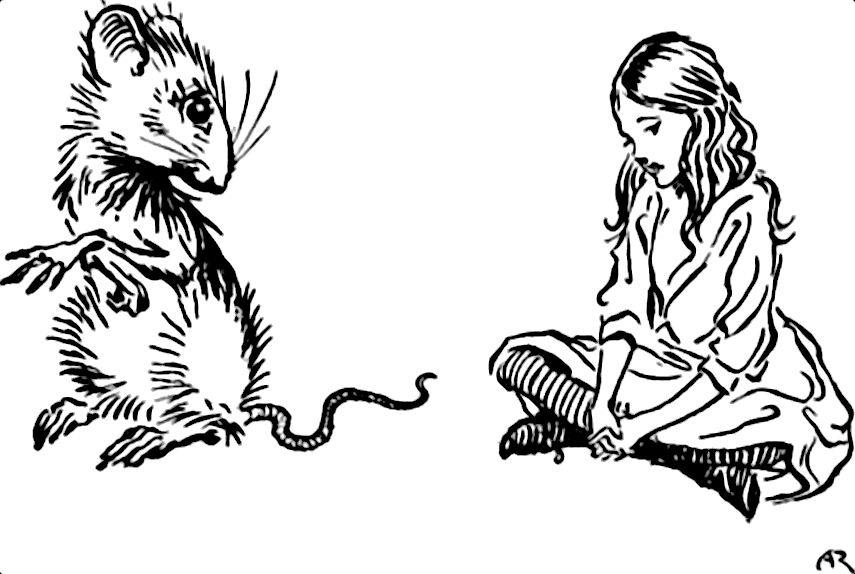
\includegraphics[width=\linewidth]{alicemouse}
\end{figure}
\vfill

\clearpage





\newgeometry{top=1cm,bottom=1cm}
\settowidth{\versewidth}{a mouse that morning}
%\indentpattern{0135554322112346898779775545653222345544456688778899}
     \indentpattern{0135554321112346899988766545653222345543456788778899}
 \begin{verse}[\versewidth]
 \setlength{\vgap}{1em}
 \begin{patverse}
 \large Fury said to \\
   a mouse, That \\
   he met \\
   in the \\
   house, \\
 \normalsize `Let us \\
   both go \\
   to law: \\
   \emph{I} will \\
   prosecute \\
   \textit{you.} --- \\
   Come, I'll \\
 \small take no \\
   denial; \\
   We must \\
   have a \\
   trial: \\
   For \\
 \footnotesize really \\
   this \\
   morning \\
   I've \\
   nothing \\
   to do.' \\
   Said the \\
   mouse to \\
 \scriptsize the cur, \\
   `Such a \\
   trial, \\
   dear sir, \\
   With no \\
   jury or \\
   judge, \\
   would be \\
   wasting \\
   our breath.' \\
 \tiny  `I'll be \\
   judge, \\
   I'll be \\
   jury.' \\
   Said \\
   cunning \\
   old Fury; \\
   `I'll try \\
   the whole \\
   cause \\
   and \\
   condemn \\
   you \\
   to \\
   death.'  \par
 \end{patverse}
 \end{verse}
 \thispagestyle{empty}
\restoregeometry
%Fury said to
%a mouse, That
%he met in the
%house, 'Let
%us both go
%to law: I
%will prose-
%cute you.—
%Come, I'll
%take no de-
%nial: We
%must have
%the trial;
%For really
%this morn-
%ing I've
%nothing
%to do.'
%Said the
%mouse to
%the cur,
%'Such a
%trial, dear
%sir, With
%no jury
%or judge,
%would
%be wast-
%ing our
%breath.'
%'I'll be
%judge,
%I'll be
%jury,'
%said
%cun-
%ning
%old
%Fury:
%'I'll
%try
%the
%whole
%cause,
%and
%con-
%demn
%you to
%death.'


»You are not attending!« said the Mouse to Alice severely. »What are you thinking of?«

»I beg your pardon,« said Alice very humbly: »you had got to the fifth bend, I think?«

»I had \textit{not!}« cried the Mouse, angrily.

»A knot!« said Alice, always ready to make herself useful, and looking anxiously about her. »Oh, do let me help to undo it!«

»I shall do nothing of the sort,« said the Mouse, getting up and walking away. »You insult me by talking such nonsense!«

»I didn't mean it!« pleaded poor Alice. »But you're so easily offended, you know!«

The Mouse only growled in reply.

»Please come back and finish your story!« Alice called after it. And the others all joined in chorus, »Yes, please do!« but the Mouse only shook its head impatiently and walked a little quicker.

»What a pity it wouldn't stay!« sighed the Lory, as soon as it was quite out of sight; and an old Crab took the opportunity of saying to her daughter, »Ah, my dear! Let this be a lesson to you never to lose \textit{your} temper!«

»Hold your tongue, Ma!« said the young Crab, a little snappishly. »You're enough to try the patience of an oyster!«

»I wish I had our Dinah here, I know I do!« said Alice aloud, addressing nobody in particular. »She'd soon fetch it back!«

»And who is Dinah, if I might venture to ask the question?« said the Lory.

Alice replied eagerly, for she was always ready to talk about her pet: »Dinah's our cat. And she's such a capital one for catching mice, you ca'n't think! And oh, I wish you could see her after the birds! Why, she'll eat a little bird as soon as look at it!«

This speech caused a remarkable sensation among the party. Some of the birds hurried off at once; one old Magpie began wrapping itself up very carefully, remarking »I really must be getting home; the night-air doesn't suit my throat!« and a Canary called out in a trembling voice to its children »Come away, my dears! It's high time you were all in bed!« On various pretexts they all moved off, and Alice was soon left alone.

»I wish I hadn't mentioned Dinah!« she said to herself in a melancholy tone. »Nobody seems to like her, down here, and I'm sure she's the best cat in the world! Oh, my dear Dinah! I wonder if I shall ever see you any more!« And here poor Alice began to cry again, for she felt very lonely and low-spirited. In a little while, however, she again heard a little pattering of footsteps in the distance, and she looked up eagerly, half hoping that the Mouse had changed his mind, and was coming back to finish his story.
%!TeX root=../alicetop.tex
\chapter{The Rabbit Sends in a Little Bill}

\lettrine[lines=4,findent=2pt]{I}{t} was the White Rabbit, trotting slowly back again, and looking anxiously about as it went, as if it had lost something; and she heard it muttering to itself, »The Duchess! The Duchess! Oh my dear paws! Oh my fur and whiskers! She'll get me executed, as sure as ferrets are ferrets! Where \textit{can} I have dropped them, I wonder?« Alice guessed in a moment that it was looking for the fan and the pair of white kid gloves, and she very good-naturedly began hunting about for them, but they were nowhere to be seen—everything seemed to have changed since her swim in the pool, and the great hall, with the glass table and the little door, had vanished completely.

Very soon the Rabbit noticed Alice, as she went hunting about, and called out to her in an angry tone, »Why, Mary Ann, what \textit{are} you doing out here? Run home this moment, and fetch me a pair of gloves and a fan! Quick, now!« And Alice was so much frightened that she ran off at once in the direction it pointed to, without trying to explain the mistake it had made.


\begin{pictures}
	\begin{letter}
		\begin{colorbigpic}
			[1.1]
			{alicerabbit}
			{»Why, Mary Ann, what \textit{are} you doing here?«}
			\end{colorbigpic}
	\end{letter}
	
	\begin{a4}
		\begin{colorbigpic}
			[1.0]
			{alicerabbit}
			{»Why, Mary Ann, what \textit{are} you doing here?«}
		\end{colorbigpic}
	\end{a4}	
\end{pictures}


»He took me for his housemaid,« she said to herself as she ran. »How surprised he'll be when he finds out who I am! But I'd better take him his fan and gloves—that is, if I can find them.« As she said this, she came upon a neat little house, on the door of which was a bright brass plate with the name »\textsc{W. Rabbit}« engraved upon it. She went in without knocking, and hurried up stairs, in great fear lest she should meet the real Mary Ann, and be turned out of the house before she had found the fan and gloves.

»How queer it seems,« Alice said to herself, »to be doing messages for a rabbit! I suppose Dinah'll be sending me on messages next!« And she began fancying the sort of thing that would happen: »'Miss Alice! Come here directly, and get ready for your walk!' 'Coming in a minute, nurse! But I've got to watch this mouse-hole till Dinah comes back, and see that the mouse doesn't get out.' Only I don't think,« Alice went on, »that they'd let Dinah stop in the house if it began ordering people about like that!«

By this time she had found her way into a tidy little room with a table in the window, and on it (as she had hoped) a fan and two or three pairs of tiny white kid gloves: she took up the fan and a pair of the gloves, and was just going to leave the room, when her eye fell upon a little bottle that stood near the looking-glass. There was no label this time with the words »\textsc{drink me},« but nevertheless she uncorked it and put it to her lips. »I know \textit{something} interesting is sure to happen,« she said to herself, »whenever I eat or drink anything; so I'll just see what this bottle does. I do hope it will make me grow large again, for really I'm quite tired of being such a tiny little thing!«

It did so indeed, and much sooner than she had expected: before she had drunk half the bottle, she found her head pressing against the ceiling, and had to stoop to save her neck from being broken. She hastily put down the bottle, saying to herself »That's quite enough—I hope I sha'n't grow any more—As it is, I can't get out at the door—I do wish I hadn't drunk quite so much!«

Alas! it was too late to wish that! She went on growing, and growing, and very soon had to kneel down on the floor: in another minute there was not even room for this, and she tried the effect of lying down with one elbow against the door, and the other arm curled round her head. Still she went on growing, and, as a last resource, she put one arm out of the window, and one foot up the chimney, and said to herself »Now I can do no more, whatever happens. What \textit{will} become of me?«

Luckily for Alice, the little magic bottle had now had its full effect, and she grew no larger: still it was very uncomfortable, and, as there seemed to be no sort of chance of her ever getting out of the room again, no wonder she felt unhappy.

»It was much pleasanter at home,« thought poor Alice, »when one wasn't always growing larger and smaller, and being ordered about by mice and rabbits. I almost wish I hadn't gone down that rabbit-hole—and yet—and yet—it's rather curious, you know, this sort of life! I do wonder what \textit{can} have happened to me! When I used to read fairy-tales, I fancied that kind of thing never happened, and now here I am in the middle of one! There ought to be a book written about me, that there ought! And when I grow up, I'll write one—but I'm grown up now,« she added in a sorrowful tone; »at least there's no room to grow up any more \textit{here}.«

»But then,« thought Alice, »shall I \textit{never} get any older than I am now? That'll be a comfort, one way—never to be an old woman—but then—always to have lessons to learn! Oh, I shouldn't like \textit{that!}«

»Oh, you foolish Alice!« she answered herself. »How can you learn lessons in here? Why, there's hardly room for \textit{you}, and no room at all for any lesson-books!«

And so she went on, taking first one side and then the other, and making quite a conversation of it altogether; but after a few minutes she heard a voice outside, and stopped to listen.

»Mary Ann! Mary Ann!« said the voice. »Fetch me my gloves this moment!« Then came a little pattering of feet on the stairs. Alice knew it was the Rabbit coming to look for her, and she trembled till she shook the house, quite forgetting that she was now about a thousand times as large as the Rabbit, and had no reason to be afraid of it.

Presently the Rabbit came up to the door, and tried to open it; but, as the door opened inwards, and Alice's elbow was pressed hard against it, that attempt proved a failure. Alice heard it say to itself »Then I'll go round and get in at the window.«

»\textit{That} you won't« thought Alice, and, after waiting till she fancied she heard the Rabbit just under the window, she suddenly spread out her hand, and made a snatch in the air. She did not get hold of anything, but she heard a little shriek and a fall, and a crash of broken glass, from which she concluded that it was just possible it had fallen into a cucumber-frame, or something of the sort.

Next came an angry voice—the Rabbit's—»Pat! Pat! Where are you?« And then a voice she had never heard before, »Sure then I'm here! Digging for apples, yer honour!«

»Digging for apples, indeed!« said the Rabbit angrily. »Here! Come and help me out of \textit{this!}« (Sounds of more broken glass.)

»Now tell me, Pat, what's that in the window?«

»Sure, it's an arm, yer honour.« (He pronounced it »arrum.«)

»An arm, you goose! Who ever saw one that size? Why, it fills the whole window!«

»Sure, it does, yer honour? but it's an arm for all that.«

»Well, it's got no business there, at any rate: go and take it away!«

There was a long silence after this, and Alice could only hear whispers now and then; such as, »Sure, I don't like it, yer honour, at all, at all!« »Do as I tell you, you coward!« and at last she spread out her hand again, and made another snatch in the air. This time there were \textit{two} little shrieks, and more sounds of broken glass. »What a number of cucumber-frames there must be!« thought Alice. »I wonder what they'll do next! As for pulling me out of the window, I only wish they \textit{could!} I'm sure \textit{I} don't want to stay in here any longer!«

She waited for some time without hearing anything more: at last came a rumbling of little cart-wheels, and the sound of a good many voices all talking together: she made out the words: »Where's the other ladder?—Why I hadn't to bring but one; Bill's got the other—Bill! Fetch it here, lad!—Here, put 'em up at this corner—No, tie 'em together first—they don't reach half high enough yet—Oh! they'll do well enough; don't be particular—Here, Bill! catch hold of this rope—Will the roof bear?—Mind that loose slate—Oh, it's coming down! Heads below!« (a loud crash)—»Now, who did that?—It was Bill, I fancy—Who's to go down the chimney?—Nay, \textit{I} sha'n't! \textit{You} do it!—\textit{That} I won't, then! Bill's to go down—Here, Bill! the master says you've to go down the chimney!«

»Oh! So Bill's got to come down the chimney, has he?« said Alice to herself. »Why, they seem to put everything upon Bill! I wouldn't be in Bill's place for a good deal: this fireplace is narrow, to be sure; but I \textit{think} I can kick a little!«

She drew her foot as far down the chimney as she could, and waited till she heard a little animal (she couldn't guess of what sort it was) scratching and scrambling about in the chimney close above her: then, saying to herself »This is Bill,« she gave one sharp kick, and waited to see what would happen next.

The first thing she heard was a general chorus of »There goes Bill!« then the Rabbit's voice alone—»Catch him, you by the hedge!« then silence, and then another confusion of voices—»Hold up his head—Brandy now—Don't choke him—How was it, old fellow? What happened to you? Tell us all about it!«

At last came a little feeble, squeaking voice, (»That's Bill,« thought Alice,) »Well, I hardly know—No more, thank ye; I'm better now—but I'm a deal too flustered to tell you—all I know is, something comes at me like a Jack-in-the-box, and up I goes like a sky-rocket!«

»So you did, old fellow!« said the others.

»We must burn the house down!« said the Rabbit's voice. And Alice called out as loud as she could, »If you do, I'll set Dinah at you!«

There was a dead silence instantly, and Alice thought to herself »I wonder what they \textit{will} do next! If they had any sense, they'd take the roof off.« After a minute or two they began moving about again, and Alice heard the Rabbit say »A barrowful will do, to begin with.«

»A barrowful of \textit{what?}« thought Alice. But she had not long to doubt, for the next moment a shower of little pebbles came rattling in at the window, and some of them hit her in the face. »I'll put a stop to this,« she said to herself, and shouted out »You'd better not do that again!« which produced another dead silence.

Alice noticed with some surprise that the pebbles were all turning into little cakes as they lay on the floor, and a bright idea came into her head. »If I eat one of these cakes,« she thought, »it's sure to make \textit{some} change in my size; and, as it can't possibly make me larger, it must make me smaller, I suppose.«

So she swallowed one of the cakes, and was delighted to find that she began shrinking directly. As soon as she was small enough to get through the door, she ran out of the house, and found quite a crowd of little animals and birds waiting outside. The poor little Lizard, Bill, was in the middle, being held up by two guinea-pigs, who were giving it something out of a bottle. They all made a rush at Alice the moment she appeared; but she ran off as hard as she could, and soon found herself safe in a thick wood.

»The first thing I've got to do,« said Alice to herself, as she wandered about in the wood, »is to grow to my right size again; and the second thing is to find my way into that lovely garden. I think that will be the best plan.«

It sounded an excellent plan, no doubt, and very neatly and simply arranged; the only difficulty was, that she had not the smallest idea how to set about it; and, while she was peering about anxiously among the trees, a little sharp bark just over her head made her look up in a great hurry.

An enormous puppy was looking down at her with large round eyes, and feebly stretching out one paw, trying to touch her. »Poor little thing!« said Alice, in a coaxing tone, and she tried hard to whistle to it; but she was terribly frightened all the time at the thought that it might be hungry, in which case it would be very likely to eat her up in spite of all her coaxing.

Hardly knowing what she did, she picked up a little bit of stick, and held it out to the puppy; whereupon the puppy jumped into the air off all its feet at once, with a yelp of delight, and rushed at the stick, and made believe to worry it; then Alice dodged behind a great thistle, to keep herself from being run over; and, the moment she appeared on the other side, the puppy made another rush at the stick, and tumbled head over heels in its hurry to get hold of it; then Alice, thinking it was very like having a game of play with a cart-horse, and expecting every moment to be trampled under its feet, ran round the thistle again; then the puppy began a series of short charges at the stick, running a little way forwards each time and a long way back, and barking hoarsely all the while, till at last it sat down a good way off, panting, with its tongue hanging out of its mouth, and its great eyes half shut.

This seemed to Alice a good opportunity for making her escape; so she set off at once, and ran till she was quite tired and out of breath, and till the puppy's bark sounded quite faint in the distance.

»And yet what a dear little puppy it was!« said Alice, as she leant against a buttercup to rest herself, and fanned herself with one of the leaves. »I should have liked teaching it tricks very much, if—if I'd only been the right size to do it! Oh, dear! I'd nearly forgotten that I've got to grow up again! Let me see—how \textit{is} it to be managed? I suppose I ought to eat or drink something or other; but the great question is, what?«

The great question certainly was, what? Alice looked all round her at the flowers and the blades of grass, but she could not see anything that looked like the right thing to eat or drink under the circumstances. There was a large mushroom growing near her, about the same height as herself; and, when she had looked under it, and on both sides of it, and behind it, it occurred to her that she might as well look and see what was on the top of it.

She stretched herself up on tiptoe, and peeped over the edge of the mushroom, and her eyes immediately met those of a large blue caterpillar, that was sitting on the top with its arms folded, quietly smoking a long hookah, and taking not the smallest notice of her or of anything else.
%!TeX root=../glasstop.tex
\chapter{Wool and Water}

\lettrine[lines=4]{S}{he} caught the shawl as she spoke, and looked about for the owner: in another moment the White Queen came running wildly through the wood, with both arms stretched out wide, as if she were flying, and Alice very civilly went to meet her with the shawl.

\label{white3}
\label{black2}

»I'm very glad I happened to be in the way,« Alice said, as she helped her to put on her shawl again.

The White Queen only looked at her in a helpless frightened sort of way, and kept repeating something in a whisper to herself that sounded like »bread-and-butter, bread-and-butter,« and Alice felt that if there was to be any conversation at all, she must manage it herself. So she began rather timidly: »Am I addressing the White Queen?«

»Well, yes, if you call that a-dressing,« The Queen said. »It isn't \textit{my} notion of the thing, at all.«

Alice thought it would never do to have an argument at the very beginning of their conversation, so she smiled and said, »If your Majesty will only tell me the right way to begin, I'll do it as well as I can.«

»But I don't want it done at all!« groaned the poor Queen. »I've been a-dressing myself for the last two hours.«

It would have been all the better, as it seemed to Alice, if she had got some one else to dress her, she was so dreadfully untidy. »Every single thing's crooked,« Alice thought to herself, »and she's all over pins!—may I put your shawl straight for you?« she added aloud.

»I don't know what's the matter with it!« the Queen said, in a melancholy voice. »It's out of temper, I think. I've pinned it here, and I've pinned it there, but there's no pleasing it!«

»It \textit{can't} go straight, you know, if you pin it all on one side,« Alice said, as she gently put it right for her; »and, dear me, what a state your hair is in!«

»The brush has got entangled in it!« the Queen said with a sigh. »And I lost the comb yesterday.«

Alice carefully released the brush, and did her best to get the hair into order. »Come, you look rather better now!« she said, after altering most of the pins. »But really you should have a lady's maid!«

»I'm sure I'll take you with pleasure!« the Queen said. »Twopence a week, and jam every other day.«

Alice couldn't help laughing, as she said, »I don't want you to hire \textit{me}—and I don't care for jam.«

»It's very good jam,« said the Queen.

»Well, I don't want any \textit{to-day,} at any rate.«

»You couldn't have it if you \textit{did} want it,« the Queen said. »The rule is, jam to-morrow and jam yesterday—but never jam to-day.«

»It \textit{must} come sometimes to »jam to-day,«« Alice objected.

»No, it can't,« said the Queen. »It's jam every \textit{other} day: to-day isn't any \textit{other} day, you know.«

»I don't understand you,« said Alice. »It's dreadfully confusing!«

»That's the effect of living backwards,« the Queen said kindly: »it always makes one a little giddy at first\longdash«

»Living backwards!« Alice repeated in great astonishment. »I never heard of such a thing!«

»—but there's one great advantage in it, that one's memory works both ways.«

»I'm sure \textit{mine} only works one way,« Alice remarked. »I can't remember things before they happen.«

»It's a poor sort of memory that only works backwards,« the Queen remarked.

»What sort of things do \textit{you} remember best?« Alice ventured to ask.

»Oh, things that happened the week after next,« the Queen replied in a careless tone. »For instance, now,« she went on, sticking a large piece of plaster on her finger as she spoke, »there's the King's Messenger. He's in prison now, being punished: and the trial doesn't even begin till next Wednesday: and of course the crime comes last of all.«

»Suppose he never commits the crime?« said Alice.

»That would be all the better, wouldn't it?« the Queen said, as she bound the plaster round her finger with a bit of ribbon.

Alice felt there was no denying \textit{that.} »Of course it would be all the better,« she said: »but it wouldn't be all the better his being punished.«

»You're wrong \textit{there,} at any rate,« said the Queen: »were \textit{you} ever punished?«

»Only for faults,« said Alice.

»And you were all the better for it, I know!« the Queen said triumphantly.

»Yes, but then I \textit{had} done the things I was punished for,« said Alice: »that makes all the difference.«

»But if you \textit{hadn't} done them,« the Queen said, »that would have been better still; better, and better, and better!« Her voice went higher with each »better,« till it got quite to a squeak at last.

Alice was just beginning to say »There's a mistake somewhere—,« when the Queen began screaming so loud that she had to leave the sentence unfinished. »Oh, oh, oh!« shouted the Queen, shaking her hand about as if she wanted to shake it off. »My finger's bleeding! Oh, oh, oh, oh!«

Her screams were so exactly like the whistle of a steam-engine, that Alice had to hold both her hands over her ears.

»What \textit{is} the matter?« she said, as soon as there was a chance of making herself heard. »Have you pricked your finger?«

»I haven't pricked it \textit{yet,}« the Queen said, »but I soon shall—oh, oh, oh!«

»When do you expect to do it?« Alice asked, feeling very much inclined to laugh.

»When I fasten my shawl again,« the poor Queen groaned out: »the brooch will come undone directly. Oh, oh!« As she said the words the brooch flew open, and the Queen clutched wildly at it, and tried to clasp it again.

»Take care!« cried Alice. »You're holding it all crooked!« And she caught at the brooch; but it was too late: the pin had slipped, and the Queen had pricked her finger.

»That accounts for the bleeding, you see,« she said to Alice with a smile. »Now you understand the way things happen here.«

»But why don't you scream now?« Alice asked, holding her hands ready to put over her ears again.

»Why, I've done all the screaming already,« said the Queen. »What would be the good of having it all over again?«

By this time it was getting light. »The crow must have flown away, I think,« said Alice: »I'm so glad it's gone. I thought it was the night coming on.«

»I wish \textit{I} could manage to be glad!« the Queen said. »Only I never can remember the rule. You must be very happy, living in this wood, and being glad whenever you like!«

»Only it is so \textit{very} lonely here!« Alice said in a melancholy voice; and at the thought of her loneliness two large tears came rolling down her cheeks.

»Oh, don't go on like that!« cried the poor Queen, wringing her hands in despair. »Consider what a great girl you are. Consider what a long way you've come to-day. Consider what o'clock it is. Consider anything, only don't cry!«

Alice could not help laughing at this, even in the midst of her tears. »Can \textit{you} keep from crying by considering things?« she asked.

»That's the way it's done,« the Queen said with great decision: »nobody can do two things at once, you know. Let's consider your age to begin with—how old are you?«

»I'm seven and a half exactly.«

»You needn't say »exactually,«« the Queen remarked: »I can believe it without that. Now I'll give \textit{you} something to believe. I'm just one hundred and one, five months and a day.«

»I can't believe \textit{that!}« said Alice.

»Can't you?« the Queen said in a pitying tone. »Try again: draw a long breath, and shut your eyes.«

Alice laughed. »There's no use trying,« she said: »one \textit{can't} believe impossible things.«

»I daresay you haven't had much practice,« said the Queen. »When I was your age, I always did it for half-an-hour a day. Why, sometimes I've believed as many as six impossible things before breakfast. There goes the shawl again!«

The brooch had come undone as she spoke, and a sudden gust of wind blew the Queen's shawl across a little brook. The Queen spread out her arms again, and went flying after it, and this time she succeeded in catching it for herself. »I've got it!« she cried in a triumphant tone. »Now you shall see me pin it on again, all by myself!«

»Then I hope your finger is better now?« Alice said very politely, as she crossed the little brook after the Queen.

»Oh, much better!« cried the Queen, her voice rising to a squeak as she went on. »Much be-etter! Be-etter! Be-e-e-etter! Be-e-ehh!« The last word ended in a long bleat, so like a sheep that Alice quite started.

She looked at the Queen, who seemed to have suddenly wrapped herself up in wool. \label{black3} Alice rubbed her eyes, and looked again. She couldn't make out what had happened at all. Was she in a shop? And was that really—was it really a \textit{sheep} that was sitting on the other side of the counter? Rub as she could, she could make nothing more of it: she was in a little dark shop, leaning with her elbows on the counter, and opposite to her was an old Sheep, sitting in an arm-chair knitting, and every now and then leaving off to look at her through a great pair of spectacles.

»What is it you want to buy?« the Sheep said at last, looking up for a moment from her knitting.

»I don't \textit{quite} know yet,« Alice said, very gently. »I should like to look all round me first, if I might.«

»You may look in front of you, and on both sides, if you like,« said the Sheep: »but you can't look \textit{all} round you—unless you've got eyes at the back of your head.«

But these, as it happened, Alice had \textit{not} got: so she contented herself with turning round, looking at the shelves as she came to them.

The shop seemed to be full of all manner of curious things—but the oddest part of it all was, that whenever she looked hard at any shelf, to make out exactly what it had on it, that particular shelf was always quite empty: though the others round it were crowded as full as they could hold.

»Things flow about so here!« she said at last in a plaintive tone, after she had spent a minute or so in vainly pursuing a large bright thing, that looked sometimes like a doll and sometimes like a work-box, and was always in the shelf next above the one she was looking at. »And this one is the most provoking of all—but I'll tell you what\longdash« she added, as a sudden thought struck her, »I'll follow it up to the very top shelf of all. It'll puzzle it to go through the ceiling, I expect!«

But even this plan failed: the »thing« went through the ceiling as quietly as possible, as if it were quite used to it.

»Are you a child or a teetotum?« the Sheep said, as she took up another pair of needles. »You'll make me giddy soon, if you go on turning round like that.« She was now working with fourteen pairs at once, and Alice couldn't help looking at her in great astonishment.

»How \textit{can} she knit with so many?« the puzzled child thought to herself. »She gets more and more like a porcupine every minute!«

»Can you row?« the Sheep asked, handing her a pair of knitting-needles as she spoke.

»Yes, a little—but not on land—and not with needles\longdash« Alice was beginning to say, when suddenly the needles turned into oars in her hands, and she found they were in a little boat, gliding along between banks: so there was nothing for it but to do her best.

»Feather!« cried the Sheep, as she took up another pair of needles.

This didn't sound like a remark that needed any answer, so Alice said nothing, but pulled away. There was something very queer about the water, she thought, as every now and then the oars got fast in it, and would hardly come out again.

»Feather! Feather!« the Sheep cried again, taking more needles. »You'll be catching a crab directly.«

»A dear little crab!« thought Alice. »I should like that.«

»Didn't you hear me say »Feather«?« the Sheep cried angrily, taking up quite a bunch of needles.

»Indeed I did,« said Alice: »you've said it very often—and very loud. Please, where \textit{are} the crabs?«

»In the water, of course!« said the Sheep, sticking some of the needles into her hair, as her hands were full. »Feather, I say!«

»\textit{Why} do you say »feather« so often?« Alice asked at last, rather vexed. »I'm not a bird!«

»You are,« said the Sheep: »you're a little goose.«

This offended Alice a little, so there was no more conversation for a minute or two, while the boat glided gently on, sometimes among beds of weeds (which made the oars stick fast in the water, worse then ever), and sometimes under trees, but always with the same tall river-banks frowning over their heads.

»Oh, please! There are some scented rushes!« Alice cried in a sudden transport of delight. »There really are—and \textit{such} beauties!«

»You needn't say »please« to \textit{me} about 'em,« the Sheep said, without looking up from her knitting: »I didn't put 'em there, and I'm not going to take 'em away.«

»No, but I meant—please, may we wait and pick some?« Alice pleaded. »If you don't mind stopping the boat for a minute.«

»How am \textit{I} to stop it?« said the Sheep. »If you leave off rowing, it'll stop of itself.«

So the boat was left to drift down the stream as it would, till it glided gently in among the waving rushes. And then the little sleeves were carefully rolled up, and the little arms were plunged in elbow-deep to get the rushes a good long way down before breaking them off—and for a while Alice forgot all about the Sheep and the knitting, as she bent over the side of the boat, with just the ends of her tangled hair dipping into the water—while with bright eager eyes she caught at one bunch after another of the darling scented rushes.

»I only hope the boat won't tipple over!« she said to herself. »Oh, \textit{what} a lovely one! Only I couldn't quite reach it.« And it certainly \textit{did} seem a little provoking (»almost as if it happened on purpose,« she thought) that, though she managed to pick plenty of beautiful rushes as the boat glided by, there was always a more lovely one that she couldn't reach.

»The prettiest are always further!« she said at last, with a sigh at the obstinacy of the rushes in growing so far off, as, with flushed cheeks and dripping hair and hands, she scrambled back into her place, and began to arrange her new-found treasures.

What mattered it to her just then that the rushes had begun to fade, and to lose all their scent and beauty, from the very moment that she picked them? Even real scented rushes, you know, last only a very little while—and these, being dream-rushes, melted away almost like snow, as they lay in heaps at her feet—but Alice hardly noticed this, there were so many other curious things to think about.

They hadn't gone much farther before the blade of one of the oars got fast in the water and \textit{wouldn't} come out again (so Alice explained it afterwards), and the consequence was that the handle of it caught her under the chin, and, in spite of a series of little shrieks of »Oh, oh, oh!« from poor Alice, it swept her straight off the seat, and down among the heap of rushes.

However, she wasn't hurt, and was soon up again: the Sheep went on with her knitting all the while, just as if nothing had happened. »That was a nice crab you caught!« she remarked, as Alice got back into her place, very much relieved to find herself still in the boat.

»Was it? I didn't see it,« Said Alice, peeping cautiously over the side of the boat into the dark water. »I wish it hadn't let go—I should so like to see a little crab to take home with me!« But the Sheep only laughed scornfully, and went on with her knitting.

»Are there many crabs here?« said Alice.

»Crabs, and all sorts of things,« said the Sheep: »plenty of choice, only make up your mind. Now, what \textit{do} you want to buy?«

\label{white4}
»To buy!« Alice echoed in a tone that was half astonished and half frightened—for the oars, and the boat, and the river, had vanished all in a moment, and she was back again in the little dark shop.

»I should like to buy an egg, please,« she said timidly. »How do you sell them?«

»Fivepence farthing for one—Twopence for two,« the Sheep replied.

»Then two are cheaper than one?« Alice said in a surprised tone, taking out her purse.

»Only you \textit{must} eat them both, if you buy two,« said the Sheep.

»Then I'll have \textit{one,} please,« said Alice, as she put the money down on the counter. For she thought to herself, »They mightn't be at all nice, you know.«

The Sheep took the money, and put it away in a box: then she said »I never put things into people's hands—that would never do—you must get it for yourself.« And so saying, she went off to the other end of the shop, and set the egg upright on a shelf.
\label{black4}

»I wonder \textit{why} it wouldn't do?« thought Alice, as she groped her way among the tables and chairs, for the shop was very dark towards the end. »The egg seems to get further away the more I walk towards it. Let me see, is this a chair? Why, it's got branches, I declare! How very odd to find trees growing here! And actually here's a little brook! Well, this is the very queerest shop I ever saw!«

So she went on, wondering more and more at every step, as everything turned into a tree the moment she came up to it, and she quite expected the egg to do the same.
%!TeX root=../alicetop.tex
\chapter{Pig and Pepper}
\lettrine[lines=4,findent=2pt]{F}{or} a minute or two she stood looking at the house, and wondering what to do next, when suddenly a footman in livery came running out of the wood—(she considered him to be a footman because he was in livery: otherwise, judging by his face only, she would have called him a fish)—and rapped loudly at the door with his knuckles. It was opened by another footman in livery, with a round face and large eyes like a frog; and both footmen, Alice noticed, had powdered hair that curled all over their heads. She felt very curious to know what it was all about, and crept a little way out of the wood to listen.

The Fish-Footman began by producing from under his arm a great letter, nearly as large as himself, and this he handed over to the other, saying, in a solemn tone, »For the Duchess. An invitation from the Queen to play croquet.« The Frog-Footman repeated, in the same solemn tone, only changing the order of the words a little, »From the Queen. An invitation for the Duchess to play croquet.«

Then they both bowed low, and their curls got entangled together.

Alice laughed so much at this, that she had to run back into the wood for fear of their hearing her; and, when she next peeped out, the Fish-Footman was gone, and the other was sitting on the ground near the door, staring stupidly up into the sky.

Alice went timidly up to the door and knocked.

»There's no use in knocking,« said the Footman, »and that for two reasons. First, because I'm on the same side of the door as you are; secondly, because they're making such a noise inside, no one could possibly hear you.« And certainly there was a most extraordinary noise going on within—a constant howling and sneezing, and every now and then a great crash, as if a dish or kettle had been broken to pieces.

»Please, then,« said Alice, »how am I to get in?«

»There might be some sense in your knocking,« the Footman went on without attending to her, »if we had the door between us. For instance, if you were \textit{inside}, you might knock, and I could let you out, you know.« He was looking up into the sky all the time he was speaking, and this Alice thought decidedly uncivil. »But perhaps he can't help it,« she said to herself: »his eyes are so \textit{very} nearly at the top of his head. But at any rate he might answer questions. How am I to get in?« she repeated aloud.

»I shall sit here,« the Footman remarked, »till to-morrow\longdash«

At this moment the door of the house opened, and a large plate came skimming out, straight at the Footman's head: it just grazed his nose, and broke to pieces against one of the trees behind him.

»—or next day, maybe,« the Footman continued in the same tone, exactly as if nothing had happened.

»How am I to get in?« asked Alice again in a louder tone.

»\textit{Are} you to get in at all?« said the Footman. »That's the first question, you know.«

\begin{letter}
	\begin{figure}[tbh]
		\centering
		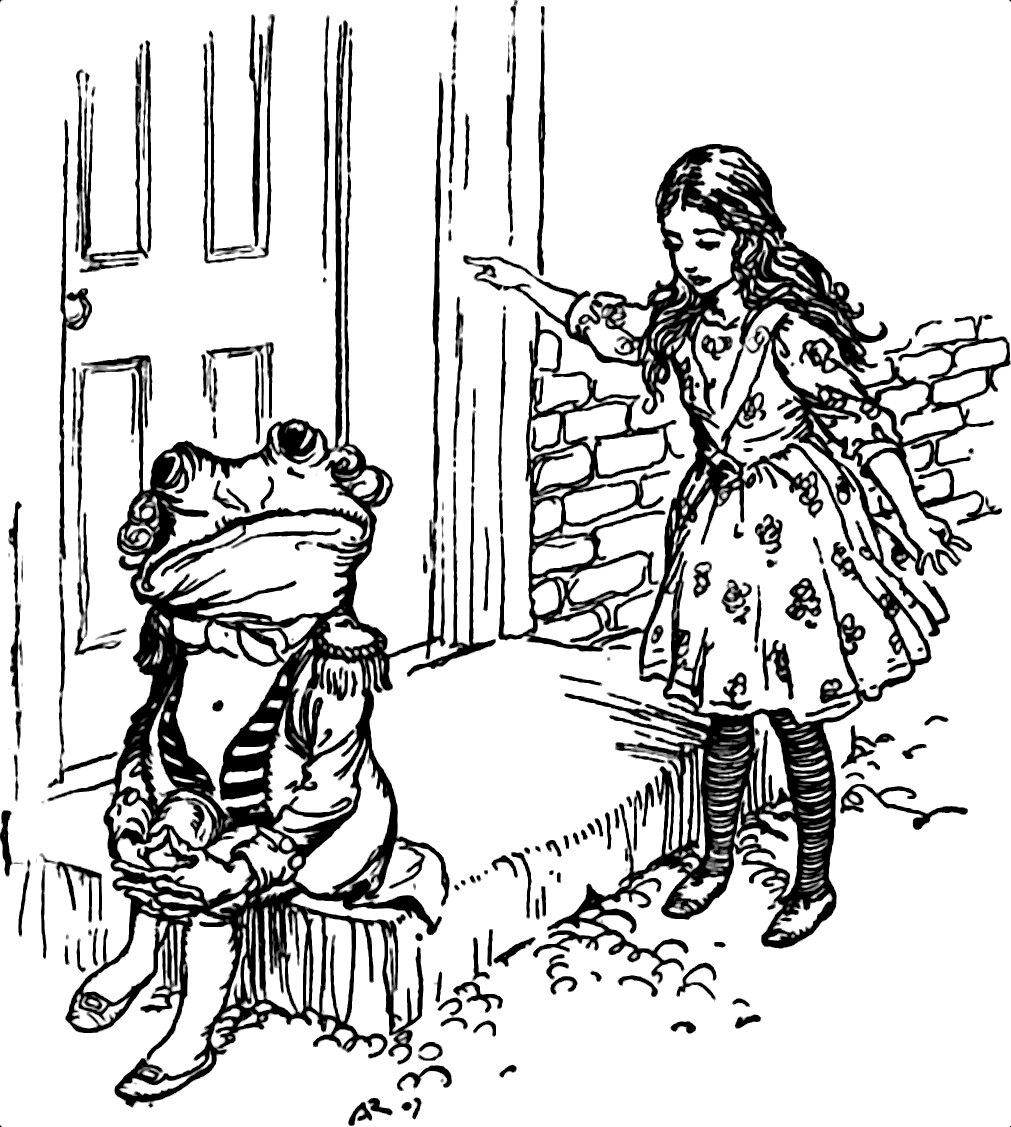
\includegraphics[width=\textwidth]{alicefrog}
	\end{figure}
\end{letter}

\begin{a4}
	\begin{figure}[tbh]
		\centering
		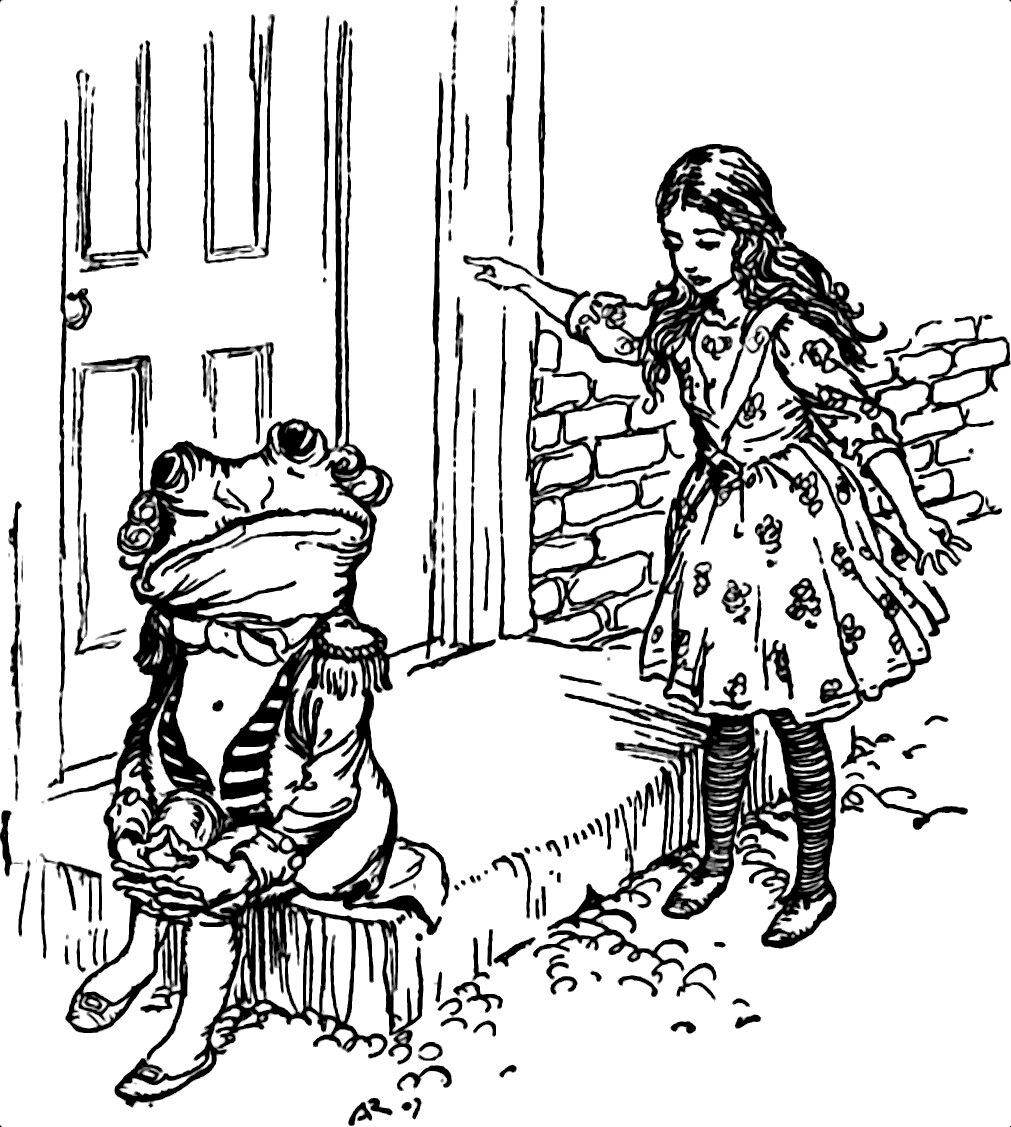
\includegraphics[width=.8\textwidth]{alicefrog}
	\end{figure}
\end{a4}


It was, no doubt: only Alice did not like to be told so. »It's really dreadful,« she muttered to herself, »the way all the creatures argue. It's enough to drive one crazy!«

The Footman seemed to consider this a good opportunity for repeating his remark, with variations. »I shall sit here,« he said, »on and off, for days and days.«

»But what am \textit{I} to do?« said Alice.

»Anything you like,« said the Footman, and began whistling.

»Oh, there's no use in talking to him,« said Alice desperately: »he's perfectly idiotic!« And she opened the door and went in.

The door led right into a large kitchen, which was full of smoke from one end to the other: the Duchess was sitting on a three-legged stool in the middle, nursing a baby, the cook was leaning over the fire, stirring a large cauldron which seemed to be full of soup.

»There's certainly too much pepper in that soup!« Alice said to herself, as well as she could for sneezing.

There was certainly too much of it in the air. Even the Duchess sneezed occasionally; and the baby was sneezing and howling alternately without a moment's pause. The only things in the kitchen that did not sneeze, were the cook, and a large cat which was sitting on the hearth and grinning from ear to ear.

»Please would you tell me,« said Alice a little timidly, for she was not quite sure whether it was good manners for her to speak first, »why your cat grins like that?«

»It's a Cheshire cat,« said the Duchess, »and that's why. Pig!«

She said the last word with such sudden violence that Alice quite jumped; but she saw in another moment that it was addressed to the baby, and not to her, so she took courage, and went on again:

»I didn't know that Cheshire cats always grinned; in fact, I didn't know that cats \textit{could} grin.«

»They all can,« said the Duchess; »and most of 'em do.«

»I don't know of any that do,« Alice said very politely, feeling quite pleased to have got into a conversation.

»You don't know much,« said the Duchess; »and that's a fact.«

Alice did not at all like the tone of this remark, and thought it would be as well to introduce some other subject of conversation. While she was trying to fix on one, the cook took the cauldron of soup off the fire, and at once set to work throwing everything within her reach at the Duchess and the baby—the fire-irons came first; then followed a shower of saucepans, plates, and dishes. The Duchess took no notice of them even when they hit her; and the baby was howling so much already, that it was quite impossible to say whether the blows hurt it or not.

»Oh, \textit{please} mind what you're doing!« cried Alice, jumping up and down in an agony of terror. »Oh, there goes his \textit{precious} nose«; as an unusually large saucepan flew close by it, and very nearly carried it off.


\begin{pictures}
	\begin{letter}
		\begin{colorbigpic}
			[1.2]
			{saucepan}
			{An unusually large saucepan flew close by it, and very nearly carried it off}
		\end{colorbigpic}
	\end{letter}
	
	\begin{a4}
		\begin{colorbigpic}
			[1.1]
			{saucepan}
			{An unusually large saucepan flew close by it, and very nearly carried it off}
		\end{colorbigpic}
	\end{a4}	
\end{pictures}


»If everybody minded their own business,« the Duchess said in a hoarse growl, »the world would go round a deal faster than it does.«


»Which would \textit{not} be an advantage,« said Alice, who felt very glad to get an opportunity of showing off a little of her knowledge. »Just think what work it would make with the day and night! You see the earth takes twenty-four hours to turn round on its axis\longdash«

»Talking of axes,« said the Duchess, »chop off her head.«

Alice glanced rather anxiously at the cook, to see if she meant to take the hint; but the cook was busily engaged in stirring the soup, and did not seem to be listening, so she ventured to go on again: »Twenty-four hours, I think; or is it twelve? I\longdash«

»Oh, don't bother \textit{me},« said the Duchess; »I never could abide figures!« And with that she began nursing her child again, singing a sort of lullaby to it as she did so, and giving it a violent shake at the end of every line:

\begin{letter}
	\pagebreak[4]
\end{letter}

\begin{verse}
	\begin{altverse}
Speak roughly to your little boy,\\
And beat him when he sneezes:\\
He only does it to annoy,\\
Because he knows it teases.\\
\end{altverse}
\end{verse}

\begin{center}
\textsc{Chorus}\\
(In which the cook and the baby joined):\\
»Wow! wow! wow!«
\end{center}

While the Duchess sang the second verse of the song, she kept tossing the baby violently up and down, and the poor little thing howled so, that Alice could hardly hear the words:

\begin{verse}
	\begin{altverse}
I speak severely to my boy,\\
I beat him when he sneezes;\\
For he can thoroughly enjoy\\
The pepper when he pleases!\\
\end{altverse}
\end{verse}

\begin{center}
\textsc{Chorus.}\\
»Wow! wow! wow!«
\end{center}

»Here! you may nurse it a bit if you like!« the Duchess said to Alice, flinging the baby at her as she spoke. »I must go and get ready to play croquet with the Queen,« and she hurried out of the room. The cook threw a frying-pan after her as she went out, but it just missed her.

Alice caught the baby with some difficulty, as it was a queer-shaped little creature, and held out its arms and legs in all directions, »just like a star-fish,« thought Alice. The poor little thing was snorting like a steam-engine when she caught it, and kept doubling itself up and straightening itself out again, so that altogether, for the first minute or two, it was as much as she could do to hold it.

As soon as she had made out the proper way of nursing it, (which was to twist it up into a knot, and then keep tight hold of its right ear and left foot, so as to prevent its undoing itself,) she carried it out into the open air. »If I don't take this child away with me,« thought Alice, »they're sure to kill it in a day or two: wouldn't it be murder to leave it behind?« She said the last words out loud, and the little thing grunted in reply (it had left off sneezing by this time). »Don't grunt,« said Alice; »that's not at all a proper way of expressing yourself.«

The baby grunted again, and Alice looked very anxiously into its face to see what was the matter with it. There could be no doubt that it had a \textit{very} turn-up nose, much more like a snout than a real nose; also its eyes were getting extremely small for a baby: altogether Alice did not like the look of the thing at all. »But perhaps it was only sobbing,« she thought, and looked into its eyes again, to see if there were any tears.

No, there were no tears. »If you're going to turn into a pig, my dear,« said Alice, seriously, »I'll have nothing more to do with you. Mind now!« The poor little thing sobbed again (or grunted, it was impossible to say which), and they went on for some while in silence.

Alice was just beginning to think to herself, »Now, what am I to do with this creature when I get it home?« when it grunted again, so violently, that she looked down into its face in some alarm. This time there could be \textit{no} mistake about it: it was neither more nor less than a pig, and she felt that it would be quite absurd for her to carry it any further.

\begin{pictures}
	\begin{letter}
		\begin{colorbigpic}
			[1.2]
			{alicepig}
			{It grunted again so violently that she looked down into its face in some alarm}
		\end{colorbigpic}
	\end{letter}
	
	\begin{a4}
		\begin{colorbigpic}
			[1.0]
			{alicepig}
			{It grunted again so violently that she looked down into its face in some alarm}
		\end{colorbigpic}
	\end{a4}	
\end{pictures}


So she set the little creature down, and felt quite relieved to see it trot quietly away into the wood. »If it had grown up,« she said to herself, »it would have made a dreadfully ugly child: but it makes rather a handsome pig, I think.« And she began thinking over other children she knew, who might do very well as pigs, and was just saying to herself, »if one only knew the right way to change them\longdash« when she was a little startled by seeing the Cheshire Cat sitting on a bough of a tree a few yards off.

The Cat only grinned when it saw Alice. It looked good-natured, she thought: still it had \textit{very} long claws and a great many teeth, so she felt that it ought to be treated with respect.



\begin{letter}
	\begin{figure}[tbh]
		\centering
		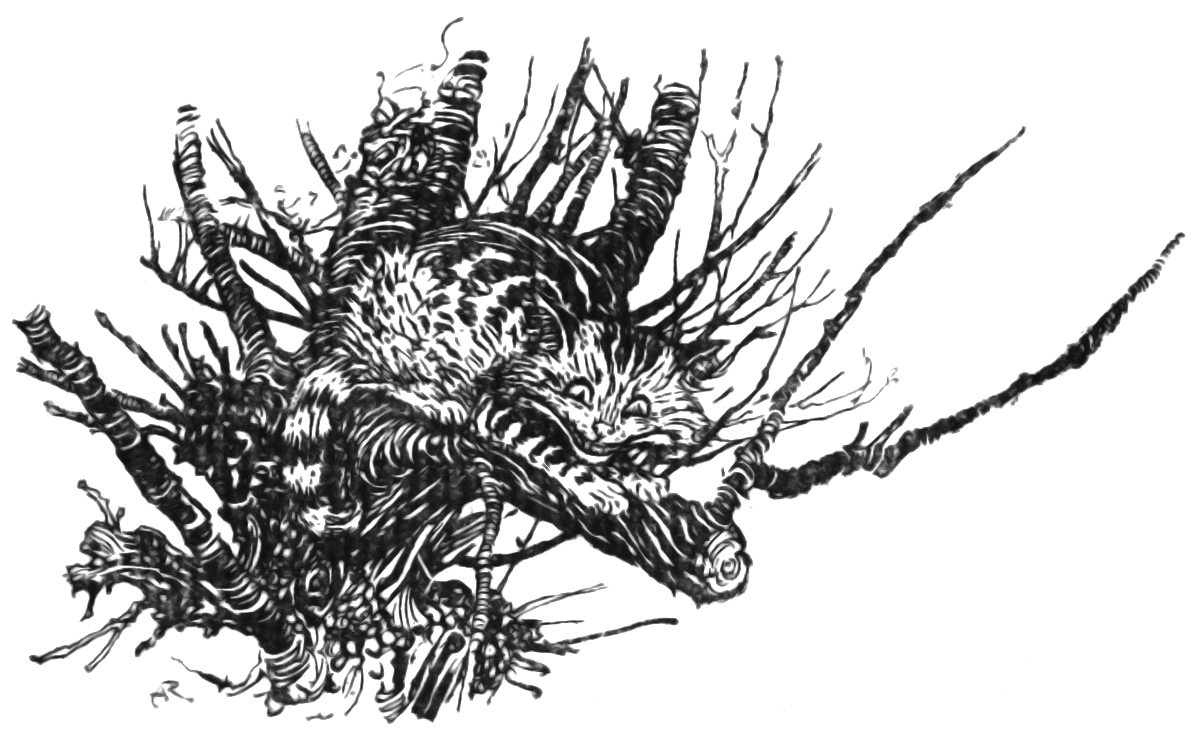
\includegraphics[width=\linewidth]{catcloseup}
	\end{figure}

\end{letter}

\begin{a4}
	\begin{figure}[tbh]
		\centering
		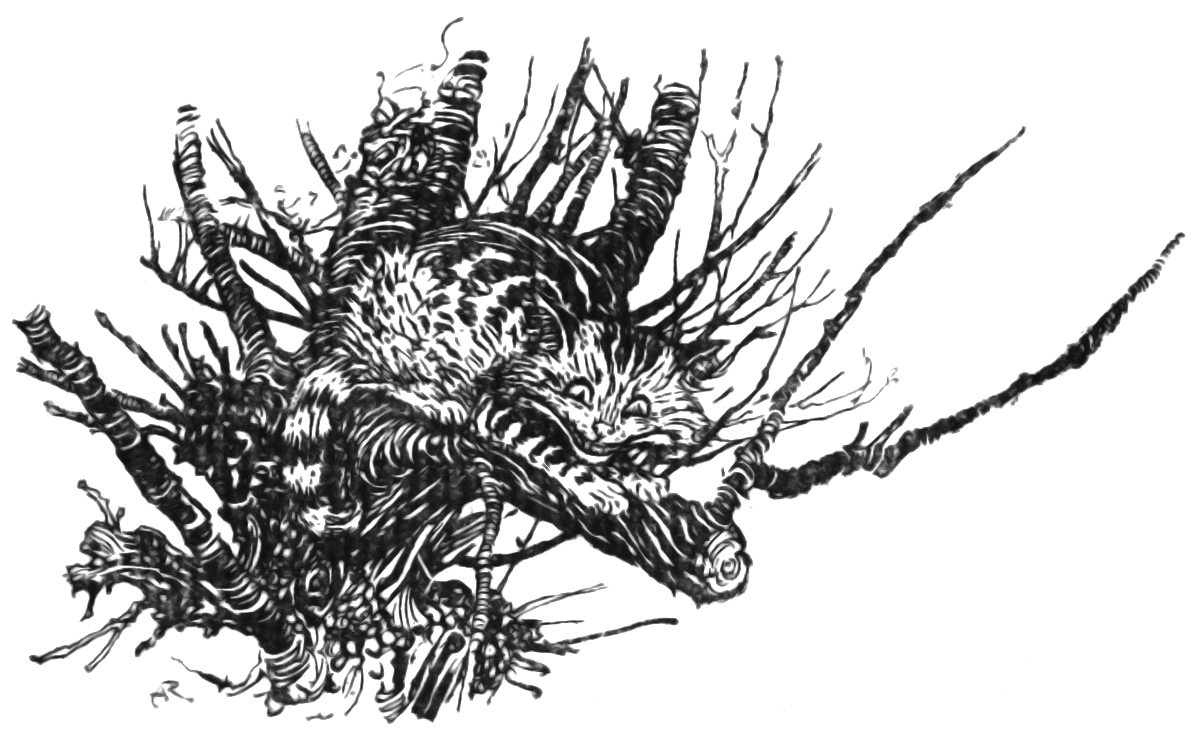
\includegraphics[width=.8\linewidth]{catcloseup}
	\end{figure}

\end{a4}

»Cheshire Puss,« she began, rather timidly, as she did not at all know whether it would like the name: however, it only grinned a little wider. »Come, it's pleased so far,« thought Alice, and she went on. »Would you tell me, please, which way I ought to go from here?«

»That depends a good deal on where you want to get to,« said the Cat.

»I don't much care where\longdash« said Alice.

»Then it doesn't matter which way you go,« said the Cat.

»— so long as I get \textit{somewhere,}« Alice added as an explanation.

»Oh, you're sure to do that,« said the Cat, »if you only walk long enough.«

Alice felt that this could not be denied, so she tried another question. »What sort of people live about here?«

»In \textit{that} direction,« the Cat said, waving its right paw round, »lives a Hatter: and in \textit{that} direction,« waving the other paw, »lives a March Hare. Visit either you like: they're both mad.«

»But I don't want to go among mad people,« Alice remarked.

»Oh, you ca'n't help that,« said the Cat: »we're all mad here. I'm mad. You're mad.«

»How do you know I'm mad?« said Alice.

»You must be,« said the Cat, »or you wouldn't have come here.«

Alice didn't think that proved it at all; however, she went on. »And how do you know that you're mad?«

»To begin with,« said the Cat, »a dog's not mad. You grant that?«

»I suppose so,« said Alice.

»Well, then,« the Cat went on, »you see a dog growls when it's angry, and wags its tail when it's pleased. Now \textit{I} growl when I'm pleased, and wag my tail when I'm angry. Therefore I'm mad.«

»\textit{I} call it purring, not growling,« said Alice.


\begin{pictures}
	\begin{letter}
		\begin{bwbigpic}
			[1.2]
			{chesirecat}
			{Sitting on a bough of a tree}
		\end{bwbigpic}
	\end{letter}
	\begin{a4}
		\begin{bwbigpic}
			[1.1]
			{chesirecat}
			{Sitting on a bough of a tree}
		\end{bwbigpic}
	\end{a4}
\end{pictures}

»Call it what you like,« said the Cat. »Do you play croquet with the Queen to-day?«

»I should like it very much,« said Alice, »but I haven't been invited yet.«

»You'll see me there,« said the Cat and vanished.

Alice was not much surprised at this, she was getting so used to queer things happening. While she was looking at the place where it had been, it suddenly appeared again.

»By-the-bye, what became of the baby?« said the Cat. »I'd nearly forgotten to ask.«

»It turned into a pig,« Alice quietly said, just as if it had come back in a natural way.

»I thought it would,« said the Cat, and vanished again.

Alice waited a little, half expecting to see it again, but it did not appear, and after a minute or two she walked on in the direction in which the March Hare was said to live. »I've seen hatters before,« she said to herself; »the March Hare will be much the most interesting, and perhaps as this is May, it won't be raving mad—at least not so mad as it was in March.« As she said this, she looked up, and there was the Cat again, sitting on the branch of a tree.

»Did you say pig, or fig?« said the Cat.

»I said pig,« replied Alice; »and I wish you wouldn't keep appearing and vanishing so suddenly: you make one quite giddy.«

»All right,« said the Cat; and this time it vanished quite slowly, beginning with the end of the tail, and ending with the grin, which remained some time after the rest of it had gone.

»Well! I've often seen a cat without a grin,« thought Alice; »but a grin without a cat! It's the most curious thing I ever saw in all my life.«


She had not gone much farther before she came in sight of the house of the March Hare: she thought it must be the right house, because the chimneys were shaped like ears and the roof was thatched with fur. It was so large a house, that she did not like to go nearer till she had nibbled some more of the left-hand bit of mushroom, and raised herself, to about two feet high: even then she walked up towards it rather timidly, saying to herself, »Suppose it should be raving mad after all! I almost wish I'd gone to see the Hatter instead!«


%!TeX root=../alicetop.tex
\chapter{A Mad Tea-party}

\lettrine[lines=4,findent=2pt]{T}{here} was a table set out under a tree in front of the house, and the March Hare and the Hatter were having tea at it: a Dormouse was sitting between them, fast asleep, and the other two were using it as a cushion resting their elbows on it, and talking over its head. »Very uncomfortable for the Dormouse,« thought Alice; »only as it's asleep, suppose it doesn't mind.«

The table was a large one, but the three were all crowded together at one corner of it. »No room! No room!« they cried out when they saw Alice coming.

»There's \textit{plenty} of room!« said Alice indignantly, and she sat down in a large arm-chair at one end of the table.

»Have some wine,« the March Hare said in an encouraging tone.

Alice looked all round the table, but there was nothing on it but tea. »I don't see any wine,« she remarked.

»There isn't any,« said the March Hare.

»Then it wasn't very civil of you to offer it,« said Alice angrily.

»It wasn't very civil of you to sit down without being invited,« said the March Hare.

»I didn't know it was \textit{your} table,« said Alice; »it's laid for a great many more than three.«

»Your hair wants cutting,« said the Hatter. He had been looking at Alice for some time with great curiosity, and this was his first speech.

»You should learn not to make personal remarks,« Alice said with some severity; »it's very rude.«

The Hatter opened his eyes very wide on hearing this; but all he \textit{said} was »Why is a raven like a writing-desk?«

»Come, we shall have some fun now!« thought Alice. »I'm glad they've begun asking riddles.—I believe I can guess that,« she added aloud.

»Do you mean that you think you can find out the answer to it?« said the March Hare.

\begin{pictures}
	\begin{letter}
		\begin{colorbigpic}
			[1.2]
			{teaparty}
			{A Mad Tea Party}
		\end{colorbigpic}
	\end{letter}
	
	\begin{a4}
		\begin{colorbigpic}
			[1.0]
			{teaparty}
			{A Mad Tea Party}
		\end{colorbigpic}
	\end{a4}	
\end{pictures}


»Exactly so,« said Alice.

»Then you should say what you mean,« the March Hare went on.

»I do,« Alice hastily replied; »at least—at least I mean what I say—that's the same thing, you know.«

»Not the same thing a bit!« said the Hatter. »Why, you might just as well say that »I see what I eat« is the same thing as »I eat what I see«!«

»You might just as well say,« added the March Hare, »that »I like what I get« is the same thing as »I get what I like«!«

»You might just as well say,« added the Dormouse, which seemed to be talking in his sleep, »that »I breathe when I sleep« is the same thing as »I sleep when I breathe«!«

»It \textit{is} the same thing with you,« said the Hatter; and here the conversation dropped, and the party sat silent for a minute, while Alice thought over all she could remember about ravens and writing-desks, which wasn't much.

The Hatter was the first to break the silence. »What day of the month is it?« he said, turning to Alice: he had taken his watch out of his pocket, and was looking at it uneasily, shaking it every now and then, and holding it to his ear.

Alice considered a little, and then said »The fourth.«

»Two days wrong!« sighed the Hatter. »I told you butter would not suit the works!« he added, looking angrily at the March Hare.

»It was the \textit{best} butter,« the March Hare meekly replied.

»Yes, but some crumbs must have got in as well,« the Hatter grumbled: »you shouldn't have put it in with the bread-knife.«

The March Hare took the watch and looked at it gloomily: then he dipped it into his cup of tea, and looked at it again: but he could think of nothing better to say than his first remark, »It was the \textit{best} butter, you know.«

Alice had been looking over his shoulder with some curiosity. »What a funny watch!« she remarked. »It tells the day of the month, and doesn't tell what o'clock it is!«

»Why should it?« muttered the Hatter. »Does \textit{your} watch tell you what year it is?«

»Of course not,« Alice replied very readily: »but that's because it stays the same year for such a long time together.«

»Which is just the case with \textit{mine},« said the Hatter.

Alice felt dreadfully puzzled. The Hatter's remark seemed to have no meaning in it, and yet it was certainly English. »I don't quite understand,« she said, as politely as she could.

»The Dormouse is asleep again,« said the Hatter, and he poured a little hot tea upon its nose.

The Dormouse shook its head impatiently, and said, without opening its eyes, »Of course, of course; just what I was going to remark myself.«

»Have you guessed the riddle yet?« the Hatter said, turning to Alice again.

»No, I give it up,« Alice replied: »what's the answer?«

»I haven't the slightest idea,« said the Hatter.

»Nor I,« said the March Hare.

Alice sighed wearily. »I think you might do something better with the time,« she said, »than wasting it asking riddles with no answers.«

»If you knew Time as well as I do,« said the Hatter, »you wouldn't talk about wasting \textit{it}. It's \textit{him}.«

»I don't know what you mean,« said Alice.

»Of course you don't!« the Hatter said, tossing his head contemptuously. »I daresay you never spoke to Time!«

»Perhaps not,« Alice cautiously replied: »but I know I have to beat time when I learn music.«

»Ah! that accounts for it,« said the Hatter. »He won't stand beating. Now, if you only kept on good terms with him, he'd do almost anything you liked with the clock. For instance, suppose it were nine o'clock in the morning, just time to begin lessons: you'd only have to whisper a hint to Time, and round goes the clock in a twinkling! Half-past one, time for dinner!«

(»I only wish it was,« the March Hare said to itself in a whisper.)

»That would be grand, certainly,« said Alice thoughtfully: »but then—I shouldn't be hungry for it, you know.«

»Not at first, perhaps,« said the Hatter: »but you could keep it to half-past one as long as you liked.«

»Is that the way \textit{you} manage?« Alice asked.

The Hatter shook his head mournfully. »Not I\@!« he replied. »We quarrelled last March—just before \textit{he} went mad, you know\longdash« (pointing with his teaspoon to the March Hare), »it was at the great concert given by the Queen of Hearts, and I had to sing

\begin{verse}
»Twinkle, twinkle, little bat!\\
How I wonder what you're at!«
\end{verse}

You know that song, perhaps?«

»I've heard something like it,« said Alice.

»It goes on, you know,« the Hatter continued, in this way:—

\begin{verse}
»Up above the world you fly,\\
Like a tea-tray in the sky.\\
\hspace{1em}Twinkle, twinkle\longdash«
\end{verse}

Here the Dormouse shook itself, and began singing in its sleep »\textit{Twinkle, twinkle, twinkle, twinkle—}« and went on so long that they had to pinch it to make it stop.

»Well, I'd hardly finished the first verse,« said the Hatter, »when the Queen jumped up and bawled out »He's murdering the time! Off with his head!««

»How dreadfully savage!« exclaimed Alice.

»And ever since that,« the Hatter went on in a mournful tone, »he won't do a thing I ask! It's always six o'clock now.«

A bright idea came into Alice's head. »Is that the reason so many tea-things are put out here?« she asked.

»Yes, that's it,« said the Hatter with a sigh: »it's always tea-time, and we've no time to wash the things between whiles.«

»Then you keep moving round, I suppose?« said Alice.

»Exactly so,« said the Hatter: »as the things get used up.«

»But what happens when you come to the beginning again?« Alice ventured to ask.

»Suppose we change the subject,« the March Hare interrupted, yawning. »I'm getting tired of this. I vote the young lady tells us a story.«

»I'm afraid I don't know one,« said Alice, rather alarmed at the proposal.

»Then the Dormouse shall!« they both cried. »Wake up, Dormouse!« And they pinched it on both sides at once.

The Dormouse slowly opened his eyes. »I wasn't asleep,« he said in a hoarse, feeble voice: »I heard every word you fellows were saying.«

»Tell us a story!« said the March Hare.

»Yes, please do!« pleaded Alice.

»And be quick about it,« added the Hatter, »or you'll be asleep again before it's done.«

»Once upon a time there were three little sisters,« the Dormouse began in a great hurry; »and their names were Elsie, Lacie, and Tillie; and they lived at the bottom of a well\longdash«

»What did they live on?« said Alice, who always took a great interest in questions of eating and drinking.

»They lived on treacle,« said the Dormouse, after thinking a minute or two.

»They couldn't have done that, you know,« Alice gently remarked; »they'd have been ill.«

»So they were,« said the Dormouse; »\textit{very} ill.«

Alice tried a little to fancy to herself what such an extraordinary way of living would be like, but it puzzled her too much, so she went on: »But why did they live at the bottom of a well?«

»Take some more tea,« the March Hare said to Alice, very earnestly.

»I've had nothing yet,« Alice replied in an offended tone, »so I can't take more.«

»You mean you can't take \textit{less},« said the Hatter; »it's very easy to take \textit{more} than nothing.«

»Nobody asked \textit{your} opinion,« said Alice.

»Who's making personal remarks now?« the Hatter asked triumphantly.

Alice did not quite know what to say to this: so she helped herself to some tea and bread-and-butter, and then turned to the Dormouse, and repeated her question. »Why did they live at the bottom of a well?«

The Dormouse again took a minute or two to think about it, and then said, »It was a treacle-well.«

»There's no such thing!« Alice was beginning very angrily, but the Hatter and the March Hare went »Sh! sh!« and the Dormouse sulkily remarked: »If you can't be civil, you'd better finish the story for yourself.«

»No, please go on!« Alice said very humbly. »I won't interrupt you again. I dare say there may be \textit{one}.«

»One, indeed!« said the Dormouse indignantly. However, he consented to go on. »And so these three little sisters—they were learning to draw, you know\longdash«

»What did they draw?« said Alice, quite forgetting her promise.

»Treacle,« said the Dormouse, without considering at all this time.

»I want a clean cup,« interrupted the Hatter: »let's all move one place on.«

He moved as he spoke, and the Dormouse followed him: the March Hare moved into the Dormouse's place, and Alice rather unwillingly took the place of the March Hare. The Hatter was the only one who got any advantage from the change: and Alice was a good deal worse off than before, as the March Hare had just upset the milk-jug into his plate.

Alice did not wish to offend the Dormouse again, so she began very cautiously: »But I don't understand. Where did they draw the treacle from?«

»You can draw water out of a water-well,« said the Hatter; »so I should think you could draw treacle out of a treacle-well—eh, stupid!«

»But they were \textit{in} the well,« Alice said to the Dormouse, not choosing to notice this last remark.

»Of course they were,« said the Dormouse; »—well in.«

This answer so confused poor Alice that she let the Dormouse go on for some time without interrupting it.

»They were learning to draw,« the Dormouse went on, yawning and rubbing its eyes, for it was getting very sleepy; »and they drew all manner of things—everything that begins with an M\longdash«

»Why with an M\@?« said Alice.

»Why not?« said the March Hare.

Alice was silent.

The Dormouse had closed its eyes by this time, and was going off into a dose; but, on being pinched by the Hatter, it woke up again with a little shriek, and went on: »— that begins with an M, such as mouse-traps, and the moon, and memory, and muchness—you know you say things are »much of a muchness«—did you ever see such a thing as a drawing of a muchness?«

»Really, now you ask me,« said Alice, very much confused, »I don't think\longdash«

»Then you shouldn't talk,« said the Hatter.

This piece of rudeness was more than Alice could bear: she got up in great disgust and walked off; the Dormouse fell asleep instantly, and neither of the others took the least notice of her going, though she looked back once or twice, half hoping that they would call after her: the last time she saw them, they were trying to put the Dormouse into the teapot.

»At any rate I'll never go \textit{there} again!« said Alice as she picked her way through the wood. »It's the stupidest tea-party I ever was at in all my life!«

Just as she said this, she noticed that one of the trees had a door leading right into it. »That's very curious!« she thought. »But everything's curious to-day. I think I may as well go in at once.« And in she went.

Once more she found herself in the long hall, and close to the little glass table. »Now I'll manage better this time,« she said to herself, and began by taking the little golden key, and unlocking the door that led into the garden. Then she set to work nibbling at the mushroom (she had kept a piece of it in her pocket) till she was about a foot high: then she walked down the little passage: and \textit{then}—she found herself at last in the beautiful garden, among the bright flower-beds and the cool fountains.
%!TeX root=../glasstop.tex
\chapter{»It's My Own Invention«}

\lettrine[lines=4]{A}{fter} a while the noise seemed gradually to die away, till all was dead silence, and Alice lifted up her head in some alarm. There was no one to be seen, and her first thought was that she must have been dreaming about the Lion and the Unicorn and those queer Anglo-Saxon Messengers. However, there was the great dish still lying at her feet, on which she had tried to cut the plum-cake, »So I wasn't dreaming, after all,« she said to herself, »unless—unless we're all part of the same dream. Only I do hope it's \textit{my} dream, and not the Red King's! I don't like belonging to another person's dream,« she went on in a rather complaining tone: »I've a great mind to go and wake him, and see what happens!«

At this moment her thoughts were interrupted by a loud shouting of »Ahoy! Ahoy! Check!« and a Knight dressed in crimson armour came galloping down upon her, brandishing a great club. Just as he reached her, the horse stopped suddenly: »You're my prisoner!« the Knight cried, as he tumbled off his horse.

Startled as she was, Alice was more frightened for him than for herself at the moment, and watched him with some anxiety as he mounted again. As soon as he was comfortably in the saddle, he began once more »You're my\longdash« but here another voice broke in »Ahoy! Ahoy! Check!« and Alice looked round in some surprise for the new enemy.

This time it was a White Knight. He drew up at Alice's side, and tumbled off his horse just as the Red Knight had done: then he got on again, and the two Knights sat and looked at each other for some time without speaking. Alice looked from one to the other in some bewilderment.

»She's \textit{my} prisoner, you know!« the Red Knight said at last.

»Yes, but then \textit{I} came and rescued her!« the White Knight replied.

»Well, we must fight for her, then,« said the Red Knight, as he took up his helmet (which hung from the saddle, and was something the shape of a horse's head), and put it on.

»You will observe the Rules of Battle, of course?« the White Knight remarked, putting on his helmet too.

»I always do,« said the Red Knight, and they began banging away at each other with such fury that Alice got behind a tree to be out of the way of the blows.

»I wonder, now, what the Rules of Battle are,« she said to herself, as she watched the fight, timidly peeping out from her hiding-place: »one Rule seems to be, that if one Knight hits the other, he knocks him off his horse, and if he misses, he tumbles off himself—and another Rule seems to be that they hold their clubs with their arms, as if they were Punch and Judy—What a noise they make when they tumble! Just like a whole set of fire-irons falling into the fender! And how quiet the horses are! They let them get on and off them just as if they were tables!«

Another Rule of Battle, that Alice had not noticed, seemed to be that they always fell on their heads, and the battle ended with their both falling off in this way, side by side: when they got up again, they shook hands, and then the Red Knight mounted and galloped off.

\label{white7}
\label{black6}

»It was a glorious victory, wasn't it?« said the White Knight, as he came up panting.

»I don't know,« Alice said doubtfully. »I don't want to be anybody's prisoner. I want to be a Queen.«

»So you will, when you've crossed the next brook,« said the White Knight. »I'll see you safe to the end of the wood—and then I must go back, you know. That's the end of my move.«

»Thank you very much,« said Alice. »May I help you off with your helmet?« It was evidently more than he could manage by himself; however, she managed to shake him out of it at last.

»Now one can breathe more easily,« said the Knight, putting back his shaggy hair with both hands, and turning his gentle face and large mild eyes to Alice. She thought she had never seen such a strange-looking soldier in all her life.

He was dressed in tin armour, which seemed to fit him very badly, and he had a queer-shaped little deal box fastened across his shoulder, upside-down, and with the lid hanging open. Alice looked at it with great curiosity.

»I see you're admiring my little box.« the Knight said in a friendly tone. »It's my own invention—to keep clothes and sandwiches in. You see I carry it upside-down, so that the rain can't get in.«

»But the things can get \textit{out,}« Alice gently remarked. »Do you know the lid's open?«

»I didn't know it,« the Knight said, a shade of vexation passing over his face. »Then all the things must have fallen out! And the box is no use without them.« He unfastened it as he spoke, and was just going to throw it into the bushes, when a sudden thought seemed to strike him, and he hung it carefully on a tree. »Can you guess why I did that?« he said to Alice.

Alice shook her head.

»In hopes some bees may make a nest in it—then I should get the honey.«

»But you've got a bee-hive—or something like one—fastened to the saddle,« said Alice.

»Yes, it's a very good bee-hive,« the Knight said in a discontented tone, »one of the best kind. But not a single bee has come near it yet. And the other thing is a mouse-trap. I suppose the mice keep the bees out—or the bees keep the mice out, I don't know which.«

»I was wondering what the mouse-trap was for,« said Alice. »It isn't very likely there would be any mice on the horse's back.«

»Not very likely, perhaps,« said the Knight: »but if they \textit{do} come, I don't choose to have them running all about.«

»You see,« he went on after a pause, »it's as well to be provided for \textit{everything}. That's the reason the horse has all those anklets round his feet.«

»But what are they for?« Alice asked in a tone of great curiosity.

»To guard against the bites of sharks,« the Knight replied. »It's an invention of my own. And now help me on. I'll go with you to the end of the wood—What's the dish for?«

»It's meant for plum-cake,« said Alice.

»We'd better take it with us,« the Knight said. »It'll come in handy if we find any plum-cake. Help me to get it into this bag.«

This took a very long time to manage, though Alice held the bag open very carefully, because the Knight was so \textit{very} awkward in putting in the dish: the first two or three times that he tried he fell in himself instead. »It's rather a tight fit, you see,« he said, as they got it in a last; »There are so many candlesticks in the bag.« And he hung it to the saddle, which was already loaded with bunches of carrots, and fire-irons, and many other things.

»I hope you've got your hair well fastened on?« he continued, as they set off.

»Only in the usual way,« Alice said, smiling.

»That's hardly enough,« he said, anxiously. »You see the wind is so \textit{very} strong here. It's as strong as soup.«

»Have you invented a plan for keeping the hair from being blown off?« Alice enquired.

»Not yet,« said the Knight. »But I've got a plan for keeping it from \textit{falling} off.«

»I should like to hear it, very much.«

»First you take an upright stick,« said the Knight. »Then you make your hair creep up it, like a fruit-tree. Now the reason hair falls off is because it hangs \textit{down}—things never fall \textit{upwards,} you know. It's a plan of my own invention. You may try it if you like.«

It didn't sound a comfortable plan, Alice thought, and for a few minutes she walked on in silence, puzzling over the idea, and every now and then stopping to help the poor Knight, who certainly was \textit{not} a good rider.

Whenever the horse stopped (which it did very often), he fell off in front; and whenever it went on again (which it generally did rather suddenly), he fell off behind. Otherwise he kept on pretty well, except that he had a habit of now and then falling off sideways; and as he generally did this on the side on which Alice was walking, she soon found that it was the best plan not to walk \textit{quite} close to the horse.

»I'm afraid you've not had much practice in riding,« she ventured to say, as she was helping him up from his fifth tumble.

The Knight looked very much surprised, and a little offended at the remark. »What makes you say that?« he asked, as he scrambled back into the saddle, keeping hold of Alice's hair with one hand, to save himself from falling over on the other side.

»Because people don't fall off quite so often, when they've had much practice.«

»I've had plenty of practice,« the Knight said very gravely: »plenty of practice!«

Alice could think of nothing better to say than »Indeed?« but she said it as heartily as she could. They went on a little way in silence after this, the Knight with his eyes shut, muttering to himself, and Alice watching anxiously for the next tumble.

»The great art of riding,« the Knight suddenly began in a loud voice, waving his right arm as he spoke, »is to keep\longdash« Here the sentence ended as suddenly as it had begun, as the Knight fell heavily on the top of his head exactly in the path where Alice was walking. She was quite frightened this time, and said in an anxious tone, as she picked him up, »I hope no bones are broken?«

»None to speak of,« the Knight said, as if he didn't mind breaking two or three of them. »The great art of riding, as I was saying, is—to keep your balance properly. Like this, you know\longdash«

He let go the bridle, and stretched out both his arms to show Alice what he meant, and this time he fell flat on his back, right under the horse's feet.

»Plenty of practice!« he went on repeating, all the time that Alice was getting him on his feet again. »Plenty of practice!«

»It's too ridiculous!« cried Alice, losing all her patience this time. »You ought to have a wooden horse on wheels, that you ought!«

»Does that kind go smoothly?« the Knight asked in a tone of great interest, clasping his arms round the horse's neck as he spoke, just in time to save himself from tumbling off again.

»Much more smoothly than a live horse,« Alice said, with a little scream of laughter, in spite of all she could do to prevent it.

»I'll get one,« the Knight said thoughtfully to himself. »One or two—several.«

There was a short silence after this, and then the Knight went on again. »I'm a great hand at inventing things. Now, I daresay you noticed, that last time you picked me up, that I was looking rather thoughtful?«

»You \textit{were} a little grave,« said Alice.

»Well, just then I was inventing a new way of getting over a gate—would you like to hear it?«

»Very much indeed,« Alice said politely.

»I'll tell you how I came to think of it,« said the Knight. »You see, I said to myself, »The only difficulty is with the feet: the \textit{head} is high enough already.« Now, first I put my head on the top of the gate—then I stand on my head—then the feet are high enough, you see—then I'm over, you see.«

»Yes, I suppose you'd be over when that was done,« Alice said thoughtfully: »but don't you think it would be rather hard?«

»I haven't tried it yet,« the Knight said, gravely: »so I can't tell for certain—but I'm afraid it \textit{would} be a little hard.«

He looked so vexed at the idea, that Alice changed the subject hastily. »What a curious helmet you've got!« she said cheerfully. »Is that your invention too?«

The Knight looked down proudly at his helmet, which hung from the saddle. »Yes,« he said, »but I've invented a better one than that—like a sugar loaf. When I used to wear it, if I fell off the horse, it always touched the ground directly. So I had a \textit{very} little way to fall, you see—But there \textit{was} the danger of falling \textit{into} it, to be sure. That happened to me once—and the worst of it was, before I could get out again, the other White Knight came and put it on. He thought it was his own helmet.«

The knight looked so solemn about it that Alice did not dare to laugh. »I'm afraid you must have hurt him,« she said in a trembling voice, »being on the top of his head.«

»I had to kick him, of course,« the Knight said, very seriously. »And then he took the helmet off again—but it took hours and hours to get me out. I was as fast as—as lightning, you know.«

»But that's a different kind of fastness,« Alice objected.

The Knight shook his head. »It was all kinds of fastness with me, I can assure you!« he said. He raised his hands in some excitement as he said this, and instantly rolled out of the saddle, and fell headlong into a deep ditch.

Alice ran to the side of the ditch to look for him. She was rather startled by the fall, as for some time he had kept on very well, and she was afraid that he really \textit{was} hurt this time. However, though she could see nothing but the soles of his feet, she was much relieved to hear that he was talking on in his usual tone. »All kinds of fastness,« he repeated: »but it was careless of him to put another man's helmet on—with the man in it, too.«

»How \textit{can} you go on talking so quietly, head downwards?« Alice asked, as she dragged him out by the feet, and laid him in a heap on the bank.

The Knight looked surprised at the question. »What does it matter where my body happens to be?« he said. »My mind goes on working all the same. In fact, the more head downwards I am, the more I keep inventing new things.«

»Now the cleverest thing of the sort that I ever did,« he went on after a pause, »was inventing a new pudding during the meat-course.«

»In time to have it cooked for the next course?« said Alice. »Well, not the \textit{next} course,« the Knight said in a slow thoughtful tone: »no, certainly not the next \textit{course.}«

»Then it would have to be the next day. I suppose you wouldn't have two pudding-courses in one dinner?«

»Well, not the \textit{next} day,« the Knight repeated as before: »not the next \textit{day.} In fact,« he went on, holding his head down, and his voice getting lower and lower, »I don't believe that pudding ever \textit{was} cooked! In fact, I don't believe that pudding ever \textit{will} be cooked! And yet it was a very clever pudding to invent.«

»What did you mean it to be made of?« Alice asked, hoping to cheer him up, for the poor Knight seemed quite low-spirited about it.

»It began with blotting paper,« the Knight answered with a groan.

»That wouldn't be very nice, I'm afraid\longdash«

»Not very nice \textit{alone,}« he interrupted, quite eagerly: »but you've no idea what a difference it makes mixing it with other things—such as gunpowder and sealing-wax. And here I must leave you.« They had just come to the end of the wood.

Alice could only look puzzled: she was thinking of the pudding.

»You are sad,« the Knight said in an anxious tone: »let me sing you a song to comfort you.«

»Is it very long?« Alice asked, for she had heard a good deal of poetry that day.

»It's long,« said the Knight, »but very, \textit{very} beautiful. Everybody that hears me sing it—either it brings the \textit{tears} into their eyes, or else\longdash«

»Or else what?« said Alice, for the Knight had made a sudden pause.

»Or else it doesn't, you know. The name of the song is called »\textit{Haddocks' Eyes}«.«

»Oh, that's the name of the song, is it?« Alice said, trying to feel interested.

»No, you don't understand,« the Knight said, looking a little vexed. »That's what the name is \textit{called}. The name really is »\textit{The Aged Aged Man}.««

»Then I ought to have said »That's what the \textit{song} is called«?« Alice corrected herself.

»No, you oughtn't: that's quite another thing! The \textit{song} is called »\textit{Ways and Means}«: but that's only what it's \textit{called,} you know!«

»Well, what \textit{is} the song, then?« said Alice, who was by this time completely bewildered.

»I was coming to that,« the Knight said. »The song really \textit{is} »\textit{A-sitting On A Gate}«: and the tune's my own invention.«

So saying, he stopped his horse and let the reins fall on its neck: then, slowly beating time with one hand, and with a faint smile lighting up his gentle foolish face, as if he enjoyed the music of his song, he began.

Of all the strange things that Alice saw in her journey Through The Looking-Glass, this was the one that she always remembered most clearly. Years afterwards she could bring the whole scene back again, as if it had been only yesterday—the mild blue eyes and kindly smile of the Knight—the setting sun gleaming through his hair, and shining on his armour in a blaze of light that quite dazzled her—the horse quietly moving about, with the reins hanging loose on his neck, cropping the grass at her feet—and the black shadows of the forest behind—all this she took in like a picture, as, with one hand shading her eyes, she leant against a tree, watching the strange pair, and listening, in a half dream, to the melancholy music of the song.

»But the tune \textit{isn't} his own invention,« she said to herself: »it's »\textit{I give thee all, I can no more}«.« She stood and listened very attentively, but no tears came into her eyes.

\begin{verse}
\needspace{2\baselineskip}
»I'll tell thee everything I can;\\
\vin There's little to relate.\\
I saw an aged aged man,\\
\vin A-sitting on a gate.\\
»Who are you, aged man?« I said,\\
\vin »and how is it you live?«\\
And his answer trickled through my head\\
\vin Like water through a sieve.

He said »I look for butterflies\\
\vin That sleep among the wheat:\\
I make them into mutton-pies,\\
\vin And sell them in the street.\\
I sell them unto men,« he said,\\
\vin »Who sail on stormy seas;\\
And that's the way I get my bread—\\
\vin A trifle, if you please.«

But I was thinking of a plan\\
\vin To dye one's whiskers green,\\
And always use so large a fan\\
\vin That they could not be seen.\\
So, having no reply to give\\
\vin To what the old man said,\\
I cried, »Come, tell me how you live!«\\
\vin And thumped him on the head.

His accents mild took up the tale:\\
\vin He said »I go my ways,\\
And when I find a mountain-rill,\\
\vin I set it in a blaze;\\
And thence they make a stuff they call\\
\vin Rolands' Macassar Oil—\\
Yet twopence-halfpenny is all\\
\vin They give me for my toil.«

\needspace{3\baselineskip}
But I was thinking of a way\\
\vin To feed oneself on batter,\\
And so go on from day to day\\
\vin Getting a little fatter.\\
I shook him well from side to side,\\
\vin Until his face was blue:\\
»Come, tell me how you live,« I cried,\\
\vin »And what it is you do!«

He said »I hunt for haddocks' eyes\\
\vin Among the heather bright,\\
And work them into waistcoat-buttons\\
\vin In the silent night.\\
And these I do not sell for gold\\
\vin Or coin of silvery shine\\
But for a copper halfpenny,\\
\vin And that will purchase nine.

I sometimes dig for buttered rolls,\\
\vin Or set limed twigs for crabs;\\
I sometimes search the grassy knolls\\
\vin For wheels of Hansom-cabs.\\
And that's the way« (he gave a wink)\\
\vin »By which I get my wealth—\\
And very gladly will I drink\\
\vin Your Honour's noble health.«

I heard him then, for I had just\\
\vin Completed my design\\
To keep the Menai bridge from rust\\
\vin By boiling it in wine.\\
I thanked him much for telling me\\
\vin The way he got his wealth,\\
But chiefly for his wish that he\\
\vin Might drink my noble health.

\needspace{3\baselineskip}
And now, if e'er by chance I put\\
\vin My fingers into glue\\
Or madly squeeze a right-hand foot\\
\vin Into a left-hand shoe,\\
Or if I drop upon my toe\\
\vin A very heavy weight,\\
I weep, for it reminds me so,\\
\vin Of that old man I used to know—\\
Whose look was mild, whose speech was slow,\\
\vin Whose hair was whiter than the snow,\\
Whose face was very like a crow,\\
\vin With eyes, like cinders, all aglow,\\
Who seemed distracted with his woe,\\
\vin Who rocked his body to and fro,\\
And muttered mumblingly and low,\\
\vin As if his mouth were full of dough,\\
Who snorted like a buffalo—\\
\vin That summer evening, long ago,\\
A-sitting on a gate.«
\end{verse}

As the Knight sang the last words of the ballad, he gathered up the reins, and turned his horse's head along the road by which they had come. »You've only a few yards to go,« he said, »down the hill and over that little brook, and then you'll be a Queen—But you'll stay and see me off first?« he added as Alice turned with an eager look in the direction to which he pointed. »I shan't be long. You'll wait and wave your handkerchief when I get to that turn in the road? I think it'll encourage me, you see.«

»Of course I'll wait,« said Alice: »and thank you very much for coming so far—and for the song—I liked it very much.«

»I hope so,« the Knight said doubtfully: »but you didn't cry so much as I thought you would.«

So they shook hands, and then the Knight rode slowly away into the forest. »It won't take long to see him \textit{off}, I expect,« Alice said to herself, as she stood watching him. »There he goes! Right on his head as usual! However, he gets on again pretty easily—that comes of having so many things hung round the horse\longdash« So she went on talking to herself, as she watched the horse walking leisurely along the road, and the Knight tumbling off, first on one side and then on the other. After the fourth or fifth tumble he reached the turn, and then she waved her handkerchief to him, and waited till he was out of sight.

»I hope it encouraged him,« she said, as she turned to run down the hill: »and now for the last brook, and to be a Queen! How grand it sounds!« A very few steps brought her to the edge of the brook. »The Eighth Square at last!« she cried as she bounded across, and threw herself down to rest on a lawn as soft as moss, with little flower-beds dotted about it here and there. »Oh, how glad I am to get here! And what \textit{is} this on my head?« she exclaimed in a tone of dismay, as she put her hands up to something very heavy, and fitted tight all round her head.

»But how \textit{can} it have got there without my knowing it?« she said to herself, as she lifted it off, and set it on her lap to make out what it could possibly be.

It was a golden crown.
\label{white8}
\label{black7}



%!TeX root=../glasstop.tex
\chapter{Queen Alice}

\lettrine[lines=4,ante=`]{W}{ell,} this \textit{is} grand!' said Alice. »I never expected I should be a Queen so soon—and I'll tell you what it is, your majesty,« she went on in a severe tone (she was always rather fond of scolding herself), »it'll never do for you to be lolling about on the grass like that! Queens have to be dignified, you know!«

So she got up and walked about—rather stiffly just at first, as she was afraid that the crown might come off: but she comforted herself with the thought that there was nobody to see her, »and if I really am a Queen,« she said as she sat down again, »I shall be able to manage it quite well in time.«

Everything was happening so oddly that she didn't feel a bit surprised at finding the Red Queen and the White Queen sitting close to her, one on each side: she would have liked very much to ask them how they came there, but she feared it would not be quite civil. However, there would be no harm, she thought, in asking if the game was over. »Please, would you tell me\longdash« she began, looking timidly at the Red Queen.

\label{black8}

»Speak when you're spoken to!« The Queen sharply interrupted her.

»But if everybody obeyed that rule,« said Alice, who was always ready for a little argument, »and if you only spoke when you were spoken to, and the other person always waited for \textit{you} to begin, you see nobody would ever say anything, so that\longdash«

»Ridiculous!« cried the Queen. »Why, don't you see, child\longdash« here she broke off with a frown, and, after thinking for a minute, suddenly changed the subject of the conversation. »What do you mean by »If you really are a Queen«? What right have you to call yourself so? You can't be a Queen, you know, till you've passed the proper examination. And the sooner we begin it, the better.«

»I only said »if«!« poor Alice pleaded in a piteous tone.

The two Queens looked at each other, and the Red Queen remarked, with a little shudder, »She \textit{says} she only said »if«\longdash«

»But she said a great deal more than that!« the White Queen moaned, wringing her hands. »Oh, ever so much more than that!«

»So you did, you know,« the Red Queen said to Alice. »Always speak the truth—think before you speak—and write it down afterwards.«

»I'm sure I didn't mean\longdash« Alice was beginning, but the Red Queen interrupted her impatiently.

»That's just what I complain of! You \textit{should} have meant! What do you suppose is the use of child without any meaning? Even a joke should have some meaning—and a child's more important than a joke, I hope. You couldn't deny that, even if you tried with both hands.«

»I don't deny things with my \textit{hands,}« Alice objected.

»Nobody said you did,« said the Red Queen. »I said you couldn't if you tried.«

»She's in that state of mind,« said the White Queen, »that she wants to deny \textit{something}—only she doesn't know what to deny!«

»A nasty, vicious temper,« the Red Queen remarked; and then there was an uncomfortable silence for a minute or two.

The Red Queen broke the silence by saying to the White Queen, »I invite you to Alice's dinner-party this afternoon.«

The White Queen smiled feebly, and said »And I invite \textit{you.}«

»I didn't know I was to have a party at all,« said Alice; »but if there is to be one, I think \textit{I} ought to invite the guests.«

»We gave you the opportunity of doing it,« the Red Queen remarked: »but I daresay you've not had many lessons in manners yet?«

»Manners are not taught in lessons,« said Alice. »Lessons teach you to do sums, and things of that sort.«

»And you do Addition?« the White Queen asked. »What's one and one and one and one and one and one and one and one and one and one?«

»I don't know,« said Alice. »I lost count.«

»She can't do Addition,« the Red Queen interrupted. »Can you do Subtraction? Take nine from eight.«

»Nine from eight I can't, you know,« Alice replied very readily: »but\longdash«

»She can't do Subtraction,« said the White Queen. »Can you do Division? Divide a loaf by a knife—what's the answer to that?«

»I suppose\longdash« Alice was beginning, but the Red Queen answered for her. »Bread-and-butter, of course. Try another Subtraction sum. Take a bone from a dog: what remains?«

Alice considered. »The bone wouldn't remain, of course, if I took it—and the dog wouldn't remain; it would come to bite me—and I'm sure \textit{I} shouldn't remain!«

»Then you think nothing would remain?« said the Red Queen.

»I think that's the answer.«

»Wrong, as usual,« said the Red Queen: »the dog's temper would remain.«

»But I don't see how\longdash«

»Why, look here!« the Red Queen cried. »The dog would lose its temper, wouldn't it?«

»Perhaps it would,« Alice replied cautiously.

»Then if the dog went away, its temper would remain!« the Queen exclaimed triumphantly.

Alice said, as gravely as she could, »They might go different ways.« But she couldn't help thinking to herself, »What dreadful nonsense we \textit{are} talking!«

»She can't do sums a \textit{bit!}« the Queens said together, with great emphasis.

»Can \textit{you} do sums?« Alice said, turning suddenly on the White Queen, for she didn't like being found fault with so much.

The Queen gasped and shut her eyes. »I can do Addition, if you give me time—but I can't do Subtraction, under \textit{any} circumstances!«

»Of course you know your A B C?« said the Red Queen.

»To be sure I do.« said Alice.

»So do I,« the White Queen whispered: »we'll often say it over together, dear. And I'll tell you a secret—I can read words of one letter! Isn't \textit{that} grand! However, don't be discouraged. You'll come to it in time.«

Here the Red Queen began again. »Can you answer useful questions?« she said. »How is bread made?«

»I know \textit{that!}« Alice cried eagerly. »You take some flour\longdash«

»Where do you pick the flower?« the White Queen asked. »In a garden, or in the hedges?«

»Well, it isn't \textit{picked} at all,« Alice explained: »it's \textit{ground}\longdash«

»How many acres of ground?« said the White Queen. »You mustn't leave out so many things.«

»Fan her head!« the Red Queen anxiously interrupted. »She'll be feverish after so much thinking.« So they set to work and fanned her with bunches of leaves, till she had to beg them to leave off, it blew her hair about so.

»She's all right again now,« said the Red Queen. »Do you know Languages? What's the French for fiddle-de-dee?«

»Fiddle-de-dee's not English,« Alice replied gravely.

»Who ever said it was?« said the Red Queen.

Alice thought she saw a way out of the difficulty this time. »If you'll tell me what language »fiddle-de-dee« is, I'll tell you the French for it!« she exclaimed triumphantly.

But the Red Queen drew herself up rather stiffly, and said »Queens never make bargains.«

»I wish Queens never asked questions,« Alice thought to herself.

»Don't let us quarrel,« the White Queen said in an anxious tone. »What is the cause of lightning?«

»The cause of lightning,« Alice said very decidedly, for she felt quite certain about this, »is the thunder—no, no!« she hastily corrected herself. »I meant the other way.«

»It's too late to correct it,« said the Red Queen: »when you've once said a thing, that fixes it, and you must take the consequences.«

»Which reminds me\longdash« the White Queen said, looking down and nervously clasping and unclasping her hands, »we had \textit{such} a thunderstorm last Tuesday—I mean one of the last set of Tuesdays, you know.«

Alice was puzzled. »In \textit{our} country,« she remarked, »there's only one day at a time.«

The Red Queen said, »That's a poor thin way of doing things. Now \textit{here,} we mostly have days and nights two or three at a time, and sometimes in the winter we take as many as five nights together—for warmth, you know.«

»Are five nights warmer than one night, then?« Alice ventured to ask.

»Five times as warm, of course.«

»But they should be five times as \textit{cold,} by the same rule\longdash«

»Just so!« cried the Red Queen. »Five times as warm, \textit{and} five times as cold—just as I'm five times as rich as you are, \textit{and} five times as clever!«

Alice sighed and gave it up. »It's exactly like a riddle with no answer!« she thought.

»Humpty Dumpty saw it too,« the White Queen went on in a low voice, more as if she were talking to herself. »He came to the door with a corkscrew in his hand\longdash«

»What did he want?« said the Red Queen.

»He said he \textit{would} come in,« the White Queen went on, »because he was looking for a hippopotamus. Now, as it happened, there wasn't such a thing in the house, that morning.«

»Is there generally?« Alice asked in an astonished tone.

»Well, only on Thursdays,« said the Queen.

»I know what he came for,« said Alice: »he wanted to punish the fish, because\longdash«

Here the White Queen began again. »It was \textit{such} a thunderstorm, you can't think!« (»She \textit{never} could, you know,« said the Red Queen.) »And part of the roof came off, and ever so much thunder got in—and it went rolling round the room in great lumps—and knocking over the tables and things—till I was so frightened, I couldn't remember my own name!«

Alice thought to herself, »I never should \textit{try} to remember my name in the middle of an accident! Where would be the use of it?« but she did not say this aloud, for fear of hurting the poor Queen's feeling.

»Your Majesty must excuse her,« the Red Queen said to Alice, taking one of the White Queen's hands in her own, and gently stroking it: »she means well, but she can't help saying foolish things, as a general rule.«

The White Queen looked timidly at Alice, who felt she \textit{ought} to say something kind, but really couldn't think of anything at the moment.

»She never was really well brought up,« the Red Queen went on: »but it's amazing how good-tempered she is! Pat her on the head, and see how pleased she'll be!« But this was more than Alice had courage to do.

»A little kindness—and putting her hair in papers—would do wonders with her\longdash«

The White Queen gave a deep sigh, and laid her head on Alice's shoulder. »I \textit{am} so sleepy?« she moaned.

»She's tired, poor thing!« said the Red Queen. »Smooth her hair—lend her your nightcap—and sing her a soothing lullaby.«

»I haven't got a nightcap with me,« said Alice, as she tried to obey the first direction: »and I don't know any soothing lullabies.«

»I must do it myself, then,« said the Red Queen, and she began:

\begin{verse}
	\begin{altverse}
Hush-a-by lady, in Alice's lap!\\
Till the feast's ready, we've time for a nap:\\
When the feast's over, we'll go to the ball—\\
Red Queen, and White Queen, and Alice, and all!
\end{altverse}
\end{verse}

»And now you know the words,« she added, as she put her head down on Alice's other shoulder, »just sing it through to \textit{me.} I'm getting sleepy, too.« In another moment both Queens were fast asleep, and snoring loud.

»What \textit{am} I to do?« exclaimed Alice, looking about in great perplexity, as first one round head, and then the other, rolled down from her shoulder, and lay like a heavy lump in her lap. »I don't think it \textit{ever} happened before, that any one had to take care of two Queens asleep at once! No, not in all the History of England—it couldn't, you know, because there never was more than one Queen at a time. Do wake up, you heavy things!« she went on in an impatient tone; but there was no answer but a gentle snoring.

The snoring got more distinct every minute, and sounded more like a tune: at last she could even make out the words, and she listened so eagerly that, when the two great heads vanished from her lap, she hardly missed them.

She was standing before an arched doorway over which were the words \textsc{Queen Alice} in large letters, and on each side of the arch there was a bell-handle; one was marked »Visitors' Bell,« and the other »Servants' Bell.«

\label{white9}
\label{black9}


»I'll wait till the song's over,« thought Alice, »and then I'll ring—the—\textit{which} bell must I ring?« she went on, very much puzzled by the names. »I'm not a visitor, and I'm not a servant. There \textit{ought} to be one marked »Queen,« you know\longdash«

Just then the door opened a little way, and a creature with a long beak put its head out for a moment and said »No admittance till the week after next!« and shut the door again with a bang.

Alice knocked and rang in vain for a long time, but at last, a very old Frog, who was sitting under a tree, got up and hobbled slowly towards her: he was dressed in bright yellow, and had enormous boots on.

»What is it, now?« the Frog said in a deep hoarse whisper.

Alice turned round, ready to find fault with anybody. »Where's the servant whose business it is to answer the door?« she began angrily.

»Which door?« said the Frog.

Alice almost stamped with irritation at the slow drawl in which he spoke. »\textit{This} door, of course!«

The Frog looked at the door with his large dull eyes for a minute: then he went nearer and rubbed it with his thumb, as if he were trying whether the paint would come off; then he looked at Alice.

»To answer the door?« he said. »What's it been asking of?« He was so hoarse that Alice could scarcely hear him.

»I don't know what you mean,« she said.

»I talks English, doesn't I?« the Frog went on. »Or are you deaf? What did it ask you?«

»Nothing!« Alice said impatiently. »I've been knocking at it!«

»Shouldn't do that—shouldn't do that\longdash« the Frog muttered. »Vexes it, you know.« Then he went up and gave the door a kick with one of his great feet. »You let \textit{it} alone,« he panted out, as he hobbled back to his tree, »and it'll let \textit{you} alone, you know.«

At this moment the door was flung open, and a shrill voice was heard singing:

\begin{verse}
»To the Looking-Glass world it was Alice that said,\\
\vin »I've a sceptre in hand, I've a crown on my head;\\
Let the Looking-Glass creatures, whatever they be,\\
\vin Come and dine with the Red Queen, the White Queen, and me.««
\end{verse}

And hundreds of voices joined in the chorus:

\begin{verse}
»Then fill up the glasses as quick as you can,\\
\vin And sprinkle the table with buttons and bran:\\
Put cats in the coffee, and mice in the tea—\\
\vin And welcome Queen Alice with thirty-times-three!«
\end{verse}

Then followed a confused noise of cheering, and Alice thought to herself, »Thirty times three makes ninety. I wonder if any one's counting?« In a minute there was silence again, and the same shrill voice sang another verse;

\begin{verse}
»»O Looking-Glass creatures,« quoth Alice, »draw near!\\
\vin 'Tis an honour to see me, a favour to hear:\\
'Tis a privilege high to have dinner and tea\\
\vin Along with the Red Queen, the White Queen, and me!««
\end{verse}

Then came the chorus again:—

\begin{verse}
»Then fill up the glasses with treacle and ink,\\
\vin Or anything else that is pleasant to drink:\\
Mix sand with the cider, and wool with the wine—\\
\vin And welcome Queen Alice with ninety-times-nine!«
\end{verse}

»Ninety times nine!« Alice repeated in despair, »Oh, that'll never be done! I'd better go in at once\longdash« and there was a dead silence the moment she appeared.

Alice glanced nervously along the table, as she walked up the large hall, and noticed that there were about fifty guests, of all kinds: some were animals, some birds, and there were even a few flowers among them. »I'm glad they've come without waiting to be asked,« she thought: »I should never have known who were the right people to invite!«

There were three chairs at the head of the table; the Red and White Queens had already taken two of them, but the middle one was empty. Alice sat down in it, rather uncomfortable in the silence, and longing for some one to speak.

\label{white10}

At last the Red Queen began. »You've missed the soup and fish,« she said. »Put on the joint!« And the waiters set a leg of mutton before Alice, who looked at it rather anxiously, as she had never had to carve a joint before.

»You look a little shy; let me introduce you to that leg of mutton,« said the Red Queen. »Alice—Mutton; Mutton—Alice.« The leg of mutton got up in the dish and made a little bow to Alice; and Alice returned the bow, not knowing whether to be frightened or amused.

»May I give you a slice?« she said, taking up the knife and fork, and looking from one Queen to the other.

»Certainly not,« the Red Queen said, very decidedly: »it isn't etiquette to cut any one you've been introduced to. Remove the joint!« And the waiters carried it off, and brought a large plum-pudding in its place.

»I won't be introduced to the pudding, please,« Alice said rather hastily, »or we shall get no dinner at all. May I give you some?«

But the Red Queen looked sulky, and growled »Pudding—Alice; Alice—Pudding. Remove the pudding!« and the waiters took it away so quickly that Alice couldn't return its bow.

However, she didn't see why the Red Queen should be the only one to give orders, so, as an experiment, she called out »Waiter! Bring back the pudding!« and there it was again in a moment like a conjuring-trick. It was so large that she couldn't help feeling a \textit{little} shy with it, as she had been with the mutton; however, she conquered her shyness by a great effort and cut a slice and handed it to the Red Queen.

»What impertinence!« said the Pudding. »I wonder how you'd like it, if I were to cut a slice out of \textit{you,} you creature!«

It spoke in a thick, suety sort of voice, and Alice hadn't a word to say in reply: she could only sit and look at it and gasp.

»Make a remark,« said the Red Queen: »it's ridiculous to leave all the conversation to the pudding!«

»Do you know, I've had such a quantity of poetry repeated to me to-day,« Alice began, a little frightened at finding that, the moment she opened her lips, there was dead silence, and all eyes were fixed upon her; »and it's a very curious thing, I think—every poem was about fishes in some way. Do you know why they're so fond of fishes, all about here?«

She spoke to the Red Queen, whose answer was a little wide of the mark. »As to fishes,« she said, very slowly and solemnly, putting her mouth close to Alice's ear, »her White Majesty knows a lovely riddle—all in poetry—all about fishes. Shall she repeat it?«

»Her Red Majesty's very kind to mention it,« the White Queen murmured into Alice's other ear, in a voice like the cooing of a pigeon. »It would be \textit{such} a treat! May I?«

»Please do,« Alice said very politely.

The White Queen laughed with delight, and stroked Alice's cheek. Then she began:

\begin{verse}
»First, the fish must be caught.«\\
\vin That is easy: a baby, I think, could have caught it.\\
»Next, the fish must be bought.«\\
\vin That is easy: a penny, I think, would have bought it.

»Now cook me the fish!«\\
\vin That is easy, and will not take more than a minute.\\
»Let it lie in a dish!«\\
\vin That is easy, because it already is in it.

»Bring it here! Let me sup!«\\
\vin It is easy to set such a dish on the table.\\
»Take the dish-cover up!«\\
\vin Ah, that is so hard that I fear I'm unable!

For it holds it like glue—\\
\vin Holds the lid to the dish, while it lies in the middle:\\
Which is easiest to do,\\
\vin Un-dish-cover the fish, or dishcover the riddle?
\end{verse}

»Take a minute to think about it, and then guess,« said the Red Queen. »Meanwhile, we'll drink your health—Queen Alice's health!« she screamed at the top of her voice, and all the guests began drinking it directly, and very queerly they managed it: some of them put their glasses upon their heads like extinguishers, and drank all that trickled down their faces—others upset the decanters, and drank the wine as it ran off the edges of the table—and three of them (who looked like kangaroos) scrambled into the dish of roast mutton, and began eagerly lapping up the gravy, »just like pigs in a trough!« thought Alice.

»You ought to return thanks in a neat speech,« the Red Queen said, frowning at Alice as she spoke.

»We must support you, you know,« the White Queen whispered, as Alice got up to do it, very obediently, but a little frightened.

»Thank you very much,« she whispered in reply, »but I can do quite well without.«

»That wouldn't be at all the thing,« the Red Queen said very decidedly: so Alice tried to submit to it with a good grace.

(»And they \textit{did} push so!« she said afterwards, when she was telling her sister the history of the feast. »You would have thought they wanted to squeeze me flat!«)

In fact it was rather difficult for her to keep in her place while she made her speech: the two Queens pushed her so, one on each side, that they nearly lifted her up into the air: »I rise to return thanks\longdash« Alice began: and she really \textit{did} rise as she spoke, several inches; but she got hold of the edge of the table, and managed to pull herself down again.

»Take care of yourself!« screamed the White Queen, seizing Alice's hair with both her hands. »Something's going to happen!«

And then (as Alice afterwards described it) all sorts of things happened in a moment. The candles all grew up to the ceiling, looking something like a bed of rushes with fireworks at the top. As to the bottles, they each took a pair of plates, which they hastily fitted on as wings, and so, with forks for legs, went fluttering about in all directions: »and very like birds they look,« Alice thought to herself, as well as she could in the dreadful confusion that was beginning.

At this moment she heard a hoarse laugh at her side, and turned to see what was the matter with the White Queen; but, instead of the Queen, there was the leg of mutton sitting in the chair. »Here I am!« cried a voice from the soup tureen, and Alice turned again, just in time to see the Queen's broad good-natured face grinning at her for a moment over the edge of the tureen, before she disappeared into the soup.

\label{black10}

There was not a moment to be lost. Already several of the guests were lying down in the dishes, and the soup ladle was walking up the table towards Alice's chair, and beckoning to her impatiently to get out of its way.

»I can't stand this any longer!« she cried as she jumped up and seized the table-cloth with both hands: one good pull, and plates, dishes, guests, and candles came crashing down together in a heap on the floor.

»And as for \textit{you,}« she went on, turning fiercely upon the Red Queen, whom she considered as the cause of all the mischief—but the Queen was no longer at her side—she had suddenly dwindled down to the size of a little doll, and was now on the table, merrily running round and round after her own shawl, which was trailing behind her.

At any other time, Alice would have felt surprised at this, but she was far too much excited to be surprised at anything \textit{now.} »As for \textit{you,}« she repeated, catching hold of the little creature in the very act of jumping over a bottle which had just lighted upon the table, »I'll shake you into a kitten, that I will!«
%!TeX root=../alicetop.tex
\chapter{The Lobster Quadrille}

\lettrine[lines=4,findent=2pt]{T}{he} Mock Turtle sighed deeply, and drew the back of one flapper across his eyes. He looked at Alice, and tried to speak, but, for a minute or two, sobs choked his voice. »Same as if he had a bone in his throat,« said the Gryphon: and it set to work shaking him and punching him in the back. At last the Mock Turtle recovered his voice, and, with tears running down his cheeks, went on again:

»You may not have lived much under the sea\longdash« (»I haven't,« said Alice) »and perhaps you were never even introduced to a lobster\longdash« (Alice began to say »I once tasted\longdash« but checked herself hastily, and said »No, never,«) »—so you can have no idea what a delightful thing a Lobster Quadrille is!«

»No, indeed,« said Alice. »What sort of a dance is it?«

»Why,« said the Gryphon, »you first form into a line along the sea-shore\longdash«

\begin{pictures}
	\begin{colorbigpic}
		[1.1]
		{turtlegryphon}
		{The two creatures sat down again, and looked at Alice}
	\end{colorbigpic}
\end{pictures}


»Two lines!« cried the Mock Turtle. »Seals, turtles, and so on; then, when you've cleared the jelly-fish out of the way\longdash«

»\textit{That} generally takes some time,« interrupted the Gryphon.

»—you advance twice\longdash«

»Each with a lobster as a partner!« cried the Gryphon.

»Of course,« the Mock Turtle said: »advance twice, set to partners\longdash«

»—change lobsters, and retire in same order,« continued the Gryphon.

»Then, you know,« the Mock Turtle went on, »you throw the\longdash«

»The lobsters!« shouted the Gryphon, with a bound into the air.

»—as far out to sea as you can\longdash«

»Swim, after them!« screamed the Gryphon.

»Turn a somersault in the sea!« cried the Mock Turtle, capering wildly about.

»Change lobsters again!« yelled the Gryphon.

»Back to land again, and—that's all the first figure,« said the Mock Turtle, suddenly dropping his voice; and the two creatures, who had been jumping about like mad things all this time, sat down again very sadly and quietly, and looked at Alice.

»It must be a very pretty dance,« said Alice, timidly.

»Would you like to see a little of it?« said the Mock Turtle.

»Very much indeed,« said Alice.

»Come, let's try the first figure!« said the Mock Turtle to the Gryphon. »We can do it without lobsters, you know. Which shall sing?«

»Oh, \textit{you} sing,« said the Gryphon. »I've forgotten the words.«

So they began solemnly dancing round and round Alice, every now and then treading on her toes when they passed too close, and waving their forepaws to mark the time, while the Mock Turtle sang this, very slowly and sadly:—

\begin{verse}
»Will you walk a little faster?« said a whiting to a snail,\\
»There's a porpoise close behind us, and he's treading on my tail.\\
See how eagerly the lobsters and the turtles all advance!\\
They are waiting on the shingle—will you come and join the dance?\\
\hspace{1em}Will you, won't you, will you, won't you, will you join the dance?\\
\hspace{1em}Will you, won't you, will you, won't you, won't you join the dance?«

»You can really have no notion how delightful it will be,\\
When they take us up and throw us, with the lobsters, out to sea!«\\
But the snail replied: »Too far, too far!« and gave a look askance—\\
Said he thanked the whiting kindly, but he would not join the dance.\\
\hspace{1em}Would not, could not, would not, could not, would not join the dance.\\
\hspace{1em}Would not, could not, would not, could not, could not join the dance.

»What matters it how far we go?« his scaly friend replied;\\
»There is another shore, you know, upon the other side.\\
The further off from England the nearer is to France—\\
Then turn not pale, beloved snail, but come and join the dance.\\
\hspace{1em}Will you, won't you, will you, won't you, will you join the dance?\\
\hspace{1em}Will you, won't you, will you, won't you, won't you join the dance?«\\
\end{verse}

»Thank you, it's a very interesting dance to watch,« said Alice, feeling very glad that it was over at last: »and I do so like that curious song about the whiting!«

»Oh, as to the whiting,« said the Mock Turtle, »they—you've seen them, of course?«

»Yes,« said Alice, »I've often seen them at dinn\longdash« she checked herself hastily.

»I don't know where Dinn may be,« said the Mock Turtle, »but if you've seen them so often, of course you know what they're like.«

»I believe so,« Alice replied thoughtfully. »They have their tails in their mouths—and they're all over crumbs.«

»You're wrong about the crumbs,« said the Mock Turtle: »crumbs would all wash off in the sea. But they \textit{have} their tails in their mouths; and the reason is\longdash« here the Mock Turtle yawned and shut his eyes. »Tell her about the reason and all that,« he said to the Gryphon.

»The reason is,« said the Gryphon, »that they \textit{would} go with the lobsters to the dance. So they got thrown out to sea. So they had to fall a long way. So they got their tails fast in their mouths. So they couldn't get them out again. That's all.«

»Thank you,« said Alice. »It's very interesting. I never knew so much about a whiting before.«

»I can tell you more than that, if you like,« said the Gryphon. »Do you know why it's called a whiting?«

»I never thought about it,« said Alice. »Why?«

»\textit{It does the boots and shoes,}« the Gryphon replied very solemnly.

Alice was thoroughly puzzled. »Does the boots and shoes!« she repeated in a wondering tone.

»Why, what are \textit{your} shoes done with?« said the Gryphon. »I mean, what makes them so shiny?«

Alice looked down at them, and considered a little before she gave her answer. »They're done with blacking, I believe.«

»Boots and shoes under the sea,« the Gryphon went on in a deep voice, »are done with whiting. Now you know.«

»And what are they made of?« Alice asked in a tone of great curiosity.

»Soles and eels, of course,« the Gryphon replied rather impatiently: »any shrimp could have told you that.«

»If I'd been the whiting,« said Alice, whose thoughts were still running on the song, »I'd have said to the porpoise,»'Keep back, please: we don't want \textit{you} with us!««

»They were obliged to have him with them,« the Mock Turtle said: »no wise fish would go anywhere without a porpoise.«

»Wouldn't it really?« said Alice in a tone of great surprise.

»Of course not,« said the Mock Turtle: »why, if a fish came to \textit{me}, and told me he was going a journey, I should say, »With what porpoise?««

»Don't you mean »purpose«?« said Alice.

»I mean what I say,« the Mock Turtle replied in an offended tone. And the Gryphon added, »Come, let's hear some of \textit{your} adventures.«


»I could tell you my adventures—beginning from this morning,« said Alice a little timidly: »but it's no use going back to yesterday, because I was a different person then.«

»Explain all that,« said the Mock Turtle.

»No, no! The adventures first,« said the Gryphon in an impatient tone: »explanations take such a dreadful time.«

So Alice began telling them her adventures from the time when she first saw the White Rabbit. She was a little nervous about it just at first, the two creatures got so close to her, one on each side, and opened their eyes and mouths so \textit{very} wide, but she gained courage as she went on. Her listeners were perfectly quiet till she got to the part about her repeating »\textit{You are old, Father William,}« to the Caterpillar, and the words all coming different, and then the Mock Turtle drew a long breath, and said, »That's very curious.«

»It's all about as curious as it can be,« said the Gryphon.

»It all came different!« the Mock Turtle repeated thoughtfully. »I should like to hear her repeat something now. Tell her to begin.« He looked at the Gryphon as if he thought it had some kind of authority over Alice.

»Stand up and repeat »\textit{'Tis the voice of the sluggard,}«« said the Gryphon.



»How the creatures order one about, and make one repeat lessons!« thought Alice. »I might as well be at school at once.« However, she got up, and began to repeat it, but her head was so full of the Lobster Quadrille, that she hardly knew what she was saying, and the words came very queer indeed:—

\begin{verse}
»'Tis the voice of the Lobster; I heard him declare,\\
»You have baked me too brown, I must sugar my hair.«\\
As a duck with its eyelids, so he with his nose\\
Trims his belt and his buttons, and turns out his toes.\\
When the sands are all dry, he is gay as a lark,\\
And will talk in contemptuous tones of the Shark:\\
But, when the tide rises and sharks are around,\\
His voice has a timid and tremulous sound.«\\
\end{verse}

»That's different from what \textit{I} used to say when I was a child,« said the Gryphon.

»Well, \textit{I} never heard it before,« said the Mock Turtle: »but it sounds uncommon nonsense.«

Alice said nothing; she had sat down with her face in her hands, wondering if anything would \textit{ever} happen in a natural way again.

»I should like to have it explained,« said the Mock Turtle.

»She ca'n't explain it,« hastily said the Gryphon. »Go on with the next verse.«

»But about his toes?« the Mock Turtle persisted. »How could he turn them out with his nose, you know?«

»It's the first position in dancing,« Alice said; but was dreadfully puzzled by the whole thing, and longed to change the subject.

»Go on with the next verse,« the Gryphon repeated: »it begins »\textit{I passed by his garden.}««

Alice did not dare to disobey, though she felt sure it would all come wrong, and she went on in a trembling voice:

\begin{verse}
»I passed by his garden, and marked, with one eye,\\
How the Owl and the Panther were sharing a pie:\\
The Panther took pie-crust, and gravy, and meat,\\
While the Owl had the dish as its share of the treat.\\
When the pie was all finished, the Owl, as a boon,\\
Was kindly permitted to pocket the spoon:\\
While the Panther received knife and fork with a growl,\\
And concluded the banquet by\longdash«\\
\end{verse}


»What \textit{is} the use of repeating all that stuff,« the Mock Turtle interrupted, »if you don't explain it as you go on? It's by far the most confusing thing \textit{I} ever heard!«

»Yes, I think you'd better leave off,« said the Gryphon: and Alice was only too glad to do so.

»Shall we try another figure of the Lobster Quadrille?« the Gryphon went on. »Or would you like the Mock Turtle to sing you another song?«

»Oh, a song, please, if the Mock Turtle would be so kind,« Alice replied, so eagerly that the Gryphon said, in a rather offended tone, »H'm! No accounting for tastes! Sing her »\textit{Turtle Soup,}« will you, old fellow?«

The Mock Turtle sighed deeply, and began, in a voice choked with sobs, to sing this:—

\begin{verse}
»Beautiful Soup, so rich and green,\\
Waiting in a hot tureen!\\
Who for such dainties would not stoop?\\
Soup of the evening, beautiful Soup!\\
Soup of the evening, beautiful Soup!\\
Beau—ootiful Soo—oop!\\
Beau—ootiful Soo—oop!\\
Soo—oop of the e—e—evening,\\
Beautiful, beautiful Soup!\\
~\\
Beautiful Soup! Who cares for fish,\\
Game, or any other dish?\\
Who would not give all else for two\\
Pennyworth only of beautiful Soup?\\
Pennyworth only of beautiful Soup?\\
Beau—ootiful Soo—oop!\\
Beau—ootiful Soo—oop!\\
Soo—oop of the e—e—evening,\\
Beautiful, beauti—\textsc{ful soup}\@!«
\end{verse}


»Chorus again!« cried the Gryphon, and the Mock Turtle had just begun to repeat it, when a cry of »The trial's beginning!« was heard in the distance.

»Come on!« cried the Gryphon, and, taking Alice by the hand, it hurried off, without waiting for the end of the song.

»What trial is it?« Alice panted as she ran; but the Gryphon only answered »Come on!« and ran the faster, while more and more faintly came, carried on the breeze that followed them, the melancholy words:—

\begin{verse}
»Soo—oop of the e—e—evening,\\
Beautiful, beautiful Soup!«
\end{verse}

\begin{figure}[bh]
\centering
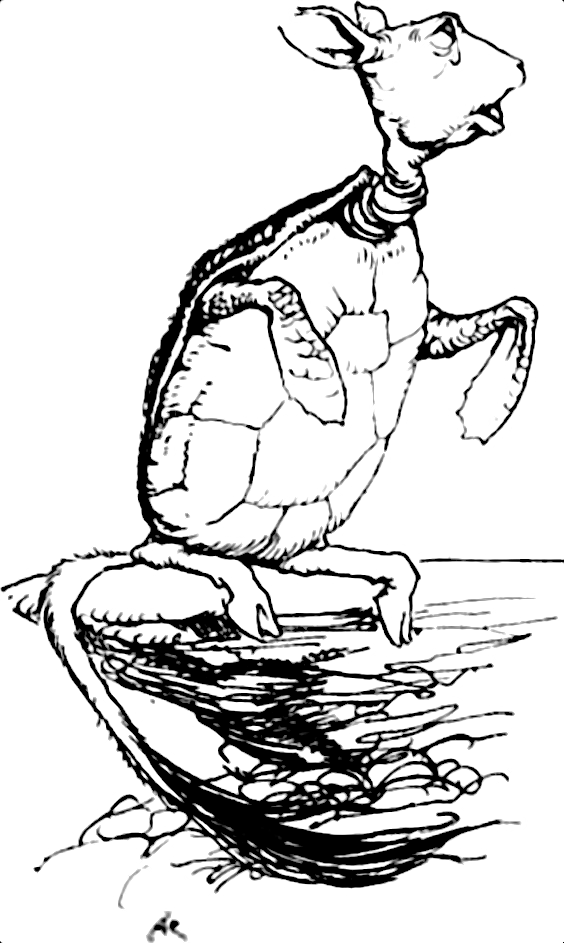
\includegraphics[width=.3\linewidth]{mockturtle}
\end{figure}
%!TeX root=../alicetop.tex
\chapter{Who Stole the Tarts?}

\lettrine[lines=4,findent=2pt]{T}{he} King and Queen of Hearts were seated on their throne when they arrived, with a great crowd assembled about them—all sorts of little birds and beasts, as well as the whole pack of cards: the Knave was standing before them, in chains, with a soldier on each side to guard him; and near the King was the White Rabbit, with a trumpet in one hand, and a scroll of parchment in the other. In the very middle of the court was a table, with a large dish of tarts upon it: they looked so good, that it made Alice quite hungry to look at them—»I wish they'd get the trial done,« she thought, »and hand round the refreshments!« But there seemed to be no chance of this, so she began looking about her, to pass away the time.

Alice had never been in a court of justice before, but she had read about them in books, and she was quite pleased to find that she knew the name of nearly everything there. »That's the judge,« she said to herself, »because of his great wig.«

The judge, by the way, was the King; and as he wore his crown over the wig, he did not look at all comfortable, and it was certainly not becoming.


\begin{pictures}
	\begin{letter}
		\begin{colorbigpic}
			[1.1]
			{court}
			{Who stole the tarts?}
		\end{colorbigpic}
	\end{letter}
	
	\begin{a4}
		\begin{colorbigpic}
			[1.0]
			{court}
			{Who stole the tarts?}
		\end{colorbigpic}
	\end{a4}	
\end{pictures}


»And that's the jury-box,« thought Alice, »and those twelve creatures,« (she was obliged to say »creatures,« you see, because some of them were animals, and some were birds,) »I suppose they are the jurors.« She said this last word two or three times over to herself, being rather proud of it: for she thought, and rightly too, that very few little girls of her age knew the meaning of it at all. However, »jurymen« would have done just as well.

The twelve jurors were all writing very busily on slates. »What are they all doing?« Alice whispered to the Gryphon. »They can't have anything to put down yet, before the trial's begun.«

»They're putting down their names,« the Gryphon whispered in reply, »for fear they should forget them before the end of the trial.«

»Stupid things!« Alice began in a loud, indignant voice, but she stopped hastily, for the White Rabbit cried out »Silence in the court!« and the King put on his spectacles and looked anxiously round, to see who was talking.

Alice could see, as well as if she were looking over their shoulders, that all the jurors were writing down »stupid things!« on their slates, and she could even make out that one of them didn't know how to spell »stupid,« and that he had to ask his neighbour to tell him. »A nice muddle their slates will be in before the trial's over!« thought Alice.

One of the jurors had a pencil that squeaked. This, of course, Alice could \textit{not} stand, and she went round the court and got behind him, and very soon found an opportunity of taking it away. She did it so quickly that the poor little juror (it was Bill, the Lizard) could not make out at all what had become of it; so, after hunting all about for it, he was obliged to write with one finger for the rest of the day; and this was of very little use, as it left no mark on the slate.

»Herald, read the accusation!« said the King.

On this the White Rabbit blew three blasts on the trumpet, and then unrolled the parchment scroll, and read as follows:

\begin{verse}
	\begin{altverse}
»The Queen of Hearts, she made some tarts,\\
All on a summer day:\\
The Knave of Hearts, he stole those tarts,\\
And took them quite away!«
\end{altverse}
\end{verse}

»Consider your verdict,« the King said to the jury.

»Not yet, not yet!« the Rabbit hastily interrupted. »There's a great deal to come before that!«

»Call the first witness,« said the King; and the Rabbit blew three blasts on the trumpet, and called out »First witness!«

The first witness was the Hatter. He came in with a teacup in one hand and a piece of bread-and-butter in the other. »I beg pardon, your Majesty,« he began, »for bringing these in; but I hadn't quite finished my tea when I was sent for.«

»You ought to have finished,« said the King. »When did you begin?«

The Hatter looked at the March Hare, who had followed him into the court, arm-in-arm with the Dormouse. »Fourteenth of March, I \textit{think} it was,« he said.

»Fifteenth,« said the March Hare.

»Sixteenth,« said the Dormouse.

»Write that down,« the King said to the jury, and the jury eagerly wrote down all three dates on their slates, and then added them up, and reduced the answer to shillings and pence.

»Take off your hat,« the King said to the Hatter.

»It isn't mine,« said the Hatter.

»\textit{Stolen!}« the King exclaimed, turning to the jury, who instantly made a memorandum of the fact.

»I keep them to sell,« the Hatter added as an explanation: »I've none of my own. I'm a hatter.«

Here the Queen put on her spectacles, and began staring hard at the Hatter, who turned pale and fidgeted.

»Give your evidence,« said the King; »and don't be nervous, or I'll have you executed on the spot.«

This did not seem to encourage the witness at all: he kept shifting from one foot to the other, looking uneasily at the Queen, and in his confusion he bit a large piece out of his teacup instead of the bread-and-butter.

Just at this moment Alice felt a very curious sensation, which puzzled her a good deal until she made out what it was: she was beginning to grow larger again, and she thought at first she would get up and leave the court; but on second thoughts she decided to remain where she was as long as there was room for her.

»I wish you wouldn't squeeze so,« said the Dormouse, who was sitting next to her. »I can hardly breathe.«

»I can't help it,« said Alice very meekly: »I'm growing.«

»You've no right to grow \textit{here},« said the Dormouse.

»Don't talk nonsense,« said Alice more boldly: »you know you're growing too.«

»Yes, but \textit{I} grow at a reasonable pace,« said the Dormouse; »not in that ridiculous fashion.« And he got up very sulkily and crossed over to the other side of the court.

All this time the Queen had never left off staring at the Hatter, and, just as the Dormouse crossed the court, she said to one of the officers of the court, »Bring me the list of the singers in the last concert!« on which the wretched Hatter trembled so, that he shook off both his shoes.

»Give your evidence,« the King repeated angrily, »or I'll have you executed, whether you're nervous or not.«

»I'm a poor man, your Majesty,« the Hatter began, in a trembling voice, »—and I hadn't begun my tea—not above a week or so—and what with the bread-and-butter getting so thin—and the twinkling of the tea\longdash«

»The twinkling of \textit{what?}« said the King.

»It \textit{began} with the tea,« the Hatter replied.

»Of course twinkling \textit{begins} with a T\@!« said the King sharply. »Do you take me for a dunce? Go on!«

»I'm a poor man,« the Hatter went on, »and most things twinkled after that—only the March Hare said\longdash«

»I didn't!« the March Hare interrupted in a great hurry.

»You did!« said the Hatter.

»I deny it!« said the March Hare.

»He denies it,« said the King: »leave out that part.«

»Well, at any rate, the Dormouse said\longdash« the Hatter went on, looking anxiously round to see if he would deny it too: but the Dormouse denied nothing, being fast asleep.

»After that,« continued the Hatter, »I cut some more bread-and-butter\longdash«

»But what did the Dormouse say?« one of the jury asked.

»That I can't remember,« said the Hatter.

»You \textit{must} remember,« remarked the King, »or I'll have you executed.«

The miserable Hatter dropped his teacup and bread-and-butter, and went down on one knee. »I'm a poor man, your Majesty,« he began.

»You're a \textit{very} poor \textit{speaker},« said the King.

Here one of the guinea-pigs cheered, and was immediately suppressed by the officers of the court. (As that is rather a hard word, I will just explain to you how it was done. They had a large canvas bag, which tied up at the mouth with strings: into this they slipped the guinea-pig, head first, and then sat upon it.)

»I'm glad I've seen that done,« thought Alice. »I've so often read in the newspapers, at the end of trials, »There was some attempt at applause, which was immediately suppressed by the officers of the court,« and I never understood what it meant till now.«

»If that's all you know about it, you may stand down,« continued the King.

»I can't go no lower,« said the Hatter: »I'm on the floor, as it is.«

»Then you may \textit{sit} down,« the King replied.

Here the other guinea-pig cheered, and was suppressed.

»Come, that finishes the guinea-pigs!« thought Alice. »Now we shall get on better.«

»I'd rather finish my tea,« said the Hatter, with an anxious look at the Queen, who was reading the list of singers.

»You may go,« said the King; and the Hatter hurriedly left the court, without even waiting to put his shoes on.

»—and just take his head off outside,« the Queen added to one of the officers; but the Hatter was out of sight before the officer could get to the door.

»Call the next witness!« said the King.

The next witness was the Duchess's cook. She carried the pepper-box in her hand, and Alice guessed who it was, even before she got into the court, by the way the people near the door began sneezing all at once.

»Give your evidence,« said the King.

»Sha'n't,« said the cook.

The King looked anxiously at the White Rabbit, who said in a low voice, »Your Majesty must cross-examine \textit{this} witness.«

»Well, if I must, I must,« the King said with a melancholy air, and, after folding his arms and frowning at the cook till his eyes were nearly out of sight, he said in a deep voice, »What are tarts made of?«

»Pepper, mostly,« said the cook.

»Treacle,« said a sleepy voice behind her.

»Collar that Dormouse,« the Queen shrieked out. »Behead that Dormouse! Turn that Dormouse out of court! Suppress him! Pinch him! Off with his whiskers.«

For some minutes the whole court was in confusion, getting the Dormouse turned out, and, by the time they had settled down again, the cook had disappeared.

»Never mind!« said the King, with an air of great relief. »Call the next witness.« And he added in an undertone to the Queen, »Really, my dear, \textit{you} must cross-examine the next witness. It quite makes my forehead ache!«

Alice watched the White Rabbit as he fumbled over the list, feeling very curious to see what the next witness would be like, »—for they haven't got much evidence \textit{yet},« she said to herself. Imagine her surprise, when the White Rabbit read out, at the top of his shrill little voice, the name »Alice!«

\begin{letter}
	
	\begin{tikzpicture}[remember picture, overlay]  
		\node (theend) at ($(current page.south)+(0cm,7cm)$) {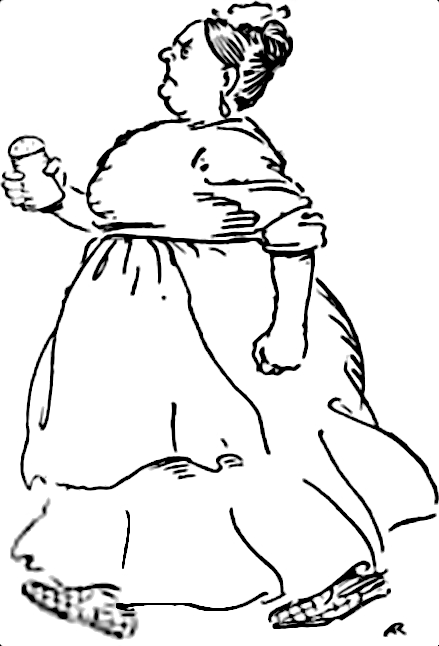
\includegraphics[width=.5\textwidth]{cook}};
	\end{tikzpicture}

\end{letter}



%!TeX root=../alicetop.tex
\chapter{Alice's Evidence}
	
\lettrine[lines=4,findent=2pt,ante=`]{H}{ere!}' cried Alice, quite forgetting in the flurry of the moment how large she had grown in the last few minutes, and she jumped up in such a hurry that she tipped over the jury-box with the edge of her skirt, upsetting all the jurymen on to the heads of the crowd below, and there they lay sprawling about, reminding her very much of a globe of gold-fish she had accidentally upset the week before.

»Oh, I \textit{beg} your pardon!« she exclaimed in a tone of great dismay, and began picking them up again as quickly as she could, for the accident of the gold-fish kept running in her head, and she had a vague sort of idea that they must be collected at once and put back into the jury-box, or they would die.

»The trial cannot proceed,« said the King in a very grave voice, »until all the jurymen are back in their proper places—\textit{all},« he repeated with great emphasis, looking hard at Alice as he said so.

Alice looked at the jury-box, and saw that, in her haste, she had put the Lizard in head downwards, and the poor little thing was waving its tail about in a melancholy way, being quite unable to move. She soon got it out again, and put it right; »not that it signifies much,« she said to herself; »I should think it would be \textit{quite} as much use in the trial one way up as the other.«

As soon as the jury had a little recovered from the shock of being upset, and their slates and pencils had been found and handed back to them, they set to work very diligently to write out a history of the accident, all except the Lizard, who seemed too much overcome to do anything but sit with its mouth open, gazing up into the roof of the court.

»What do you know about this business?« the King said to Alice.

»Nothing,« said Alice.

»Nothing \textit{whatever?}« persisted the King.

»Nothing whatever,« said Alice.

»That's very important,« the King said, turning to the jury. They were just beginning to write this down on their slates, when the White Rabbit interrupted: »\textit{Un}important, your Majesty means, of course,« he said in a very respectful tone, but frowning and making faces at him as he spoke.

»\textit{Un}important, of course, I meant,« the King hastily said, and went on himself in an undertone, »important—unimportant—unimportant—important\longdash« as if he were trying which word sounded best.

Some of the jury wrote it down »important,« and some »unimportant.« Alice could see this, as she was near enough to look over their slates; »but it doesn't matter a bit,« she thought to herself.

At this moment the King, who had been for some time busily writing in his note-book, called out »Silence!« and read out from his book, »Rule Forty-two. \textit{All persons more than a mile high to leave the court.}«

Everybody looked at Alice.

»\textit{I'm} not a mile high,« said Alice.

»You are,« said the King.

»Nearly two miles high,« added the Queen.

»Well, I sha'n't go, at any rate,« said Alice: »besides, that's not a regular rule: you invented it just now.«

»It's the oldest rule in the book,« said the King.

»Then it ought to be Number One,« said Alice.

The King turned pale, and shut his note-book hastily. »Consider your verdict,« he said to the jury, in a low trembling voice.

»There's more evidence to come yet, please your Majesty,« said the White Rabbit, jumping up in a great hurry: »this paper has just been picked up.«

»What's in it?« said the Queen.

»I haven't opened it yet,« said the White Rabbit, »but it seems to be a letter, written by the prisoner to—to somebody.«

»It must have been that,« said the King, »unless it was written to nobody, which isn't usual, you know.«

»Who is it directed to?« said one of the jurymen.

»It isn't directed at all,« said the White Rabbit; »in fact, there's nothing written on the \textit{outside}.« He unfolded the paper as he spoke, and added »It isn't a letter after all: it's a set of verses.«

»Are they in the prisoner's handwriting?« asked another of the jurymen.

»No, they're not,« said the White Rabbit, »and that's the queerest thing about it.« (The jury all looked puzzled.)

»He must have imitated somebody else's hand,« said the King. (The jury all brightened up again.)

»Please your Majesty,« said the Knave, »I didn't write it, and they can't prove that I did: there's no name signed at the end.«

»If you didn't sign it,« said the King, »that only makes the matter worse. You \textit{must} have meant some mischief, or else you'd have signed your name like an honest man.«

There was a general clapping of hands at this: it was the first really clever thing the King had said that day.

»That \textit{proves} his guilt, of course,« said the Queen: »so, off with\longdash«

»It doesn't prove anything of the sort!« said Alice. »Why, you don't even know what they're about!«

»Read them,« said the King.

The White Rabbit put on his spectacles. »Where shall I begin, please your Majesty?« he asked.

»Begin at the beginning,« the King said gravely, »and go on till you come to the end; then stop.«

There was dead silence in the court, whilst the White Rabbit read out these verses:—

%\settowidth{\versewidth}{Don't let him know she liked them best,}
\begin{verse}
»They told me you had been to her,\\
\vin And mentioned me to him:\\
She gave me a good character,\\
\vin But said I could not swim.

He sent them word I had not gone,\\
\vin (We know it to be true):\\
If she should push the matter on,\\
\vin What would become of you?

I gave her one, they gave him two,\\
\vin You gave us three or more;\\
They all returned from him to you,\\
\vin Though they were mine before.

If I or she should chance to be\\
\vin Involved in this affair,\\
He trusts to you to set them free,\\
\vin Exactly as we were.

My notion was that you had been\\
\vin  (Before she had this fit)\\
An obstacle that came between\\
\vin  Him, and ourselves, and it.

Don't let him know she liked them best,\\
\vin  For this must ever be\\
A secret, kept from all the rest,\\
\vin  Between yourself and me.«
\end{verse}

»That's the most important piece of evidence we've heard yet,« said the King, rubbing his hands; »so now let the jury\longdash«

»If any of them can explain it,« said Alice, (she had grown so large in the last few minutes that she wasn't a bit afraid of interrupting him,) »I'll give him sixpence. \textit{I} don't believe there's an atom of meaning in it.«

The jury all wrote down on their slates, »\textit{She} doesn't believe there's an atom of meaning in it,« but none of them attempted to explain the paper.

»If there's no meaning in it,« said the King, »that saves a world of trouble, you know, as we needn't try to find any. And yet I don't know,« he went on, spreading out the verses on his knee, and looking at them with one eye; »I seem to see some meaning in them after all. »—\textit{said I could not swim}\longdash« you can't swim can you?« he added, turning to the Knave.

The Knave shook his head sadly. »Do I look like it?« he said. (Which he certainly did \textit{not}, being made entirely of cardboard.)

»All right, so far,« said the King, as he went on muttering over the verses to himself: »»\textit{We know it to be true—}« that's the jury, of course—»\textit{If she should push the matter on}«—that must be the Queen—»\textit{What would become of you?}«—What, indeed!—»\textit{I gave her one, they gave him two—}« why, that must be what he did with the tarts, you know\longdash«

»But it goes on »\textit{they all returned from him to you,}«« said Alice.

»Why, there they are!« said the King triumphantly, pointing to the tarts on the table. »Nothing can be clearer than \textit{that}. Then again—»\textit{before she had this fit—}« you never had \textit{fits}, my dear, I think?« he said to the Queen.

»Never!« said the Queen furiously, throwing an inkstand at the Lizard as she spoke. (The unfortunate little Bill had left off writing on his slate with one finger, as he found it made no mark; but he now hastily began again, using the ink, that was trickling down his face, as long as it lasted.)


»Then the words don't \textit{fit} you,« said the King, looking round the court with a smile. There was a dead silence.

»It's a pun!« the King added in an angry tone, and everybody laughed.

»Let the jury consider their verdict,« the King said, for about the twentieth time that day.

»No, no!« said the Queen. »Sentence first—verdict afterwards.«

»Stuff and nonsense!« said Alice loudly. »The idea of having the sentence first!«

»Hold your tongue!« said the Queen, turning purple.

»I won't!« said Alice.

»Off with her head!« the Queen shouted at the top of her voice. Nobody moved.

»Who cares for \textit{you?}« said Alice (she had grown to her full size by this time). »You're nothing but a pack of cards!«

\begin{pictures}
	\begin{letter}
		\begin{colorbigpic}
			[1.1]
			{packofcards}
			{»You're nothing but a pack of cards!«}
		\end{colorbigpic}
	\end{letter}
	
	\begin{a4}
		\begin{colorbigpic}
			[1.0]
			{packofcards}
			{»You're nothing but a pack of cards!«}
		\end{colorbigpic}
	\end{a4}	
\end{pictures}


At this the whole pack rose up into the air, and came flying down upon her: she gave a little scream, half of fright and half of anger, and tried to beat them off, and found herself lying on the bank, with her head in the lap of her sister, who was gently brushing away some dead leaves that had fluttered down from the trees upon her face.

»Wake up, Alice dear!« said her sister. »Why, what a long sleep you've had!«

»Oh, I've had such a curious dream!« said Alice, and she told her sister, as well as she could remember them, all these strange Adventures of hers that you have just been reading about; and when she had finished, her sister kissed her, and said »It \textit{was} a curious dream, dear, certainly: but now run in to your tea; it's getting late.« So Alice got up and ran off, thinking while she ran, as well she might, what a wonderful dream it had been.


\divider



But her sister sat still just as she had left her, leaning her head, watching the setting sun, and thinking of little Alice and all her wonderful Adventures, till she too began dreaming after a fashion, and this was her dream:

First, she dreamed of little Alice herself, and once again the tiny hands were clasped upon her knee, and the bright eager eyes were looking up into hers—she could hear the very tones of her voice, and see that queer little toss of her head to keep back the wandering hair that \textit{would} always get into her eyes—and still as she listened, or seemed to listen, the whole place around her became alive with the strange creatures of her little sister's dream.

The long grass rustled at her feet as the White Rabbit hurried by—the frightened Mouse splashed his way through the neighbouring pool—she could hear the rattle of the teacups as the March Hare and his friends shared their never-ending meal, and the shrill voice of the Queen ordering off her unfortunate guests to execution—once more the pig-baby was sneezing on the Duchess' knee, while plates and dishes crashed around it—once more the shriek of the Gryphon, the squeaking of the Lizard's slate-pencil, and the choking of the suppressed guinea-pigs, filled the air, mixed up with the distant sobs of the miserable Mock Turtle.

So she sat on with closed eyes, and half believed herself in Wonderland, though she knew she had but to open them again, and all would change to dull reality—the grass would be only rustling in the wind, and the pool rippling to the waving of the reeds—the rattling teacups would change to the tinkling sheep-bells, and the Queen's shrill cries to the voice of the shepherd boy—and the sneeze of the baby, the shriek of the Gryphon, and all the other queer noises, would change (she knew) to the confused clamour of the busy farm-yard—while the lowing of the cattle in the distance would take the place of the Mock Turtle's heavy sobs.

Lastly, she pictured to herself how this same little sister of hers would, in the after-time, be herself a grown woman; and how she would keep, through all her riper years, the simple and loving heart of her childhood: and how she would gather about her other little children, and make \textit{their} eyes bright and eager with many a strange tale, perhaps even with the dream of Wonderland of long ago: and how she would feel with all their simple sorrows, and find a pleasure in all their simple joys, remembering her own child-life, and the happy summer days.

\vfill
\centerline{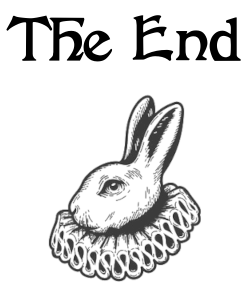
\includegraphics[width=0.4\textwidth]{end}}
\vfill



\KOMAoptions{headings=openright}


\renewcommand*{\chapterheadendvskip}{\vfill}
\renewcommand*{\chapterheadstartvskip}{\vfill}

\KOMAoptions{headings=openleft}
\chapter*{Colophon}

\centering

\vfill
\begin{minipage}{\textwidth}
\textit{Through the Looking Glass} was first published in December 1871 by Macmillan in London (UK). Like its predecessor \textit{Alice's Adventures in Wonderland}, author Charles Lutwidge Dodgson (1832\textendash 1898), a maths professor at Oxford University, wrote it for the middle daughter of his close friend Henry Lidell (Alice Lidell, 10 when \textit{Alice's Adventures in Wonderland} was written) and published it under his pen name »Lewis Carroll«.
\end{minipage}
\vfill
gutenberg.org/ebooks/12
\vfill
\divider
\vfill
\begin{minipage}{\textwidth}
Text is set in »EB Garamond,« Georg Mayr-Duffner's free and open source implementation of Claude Garamond’s famous humanist typefaces from the mid-sixteenth century. Chapter dropcaps are set in »Roycroft Initials«, by Dieter Steffmann. Title page is set in »Fantaisie Artistique,« by George Williams. 
\end{minipage}
\vfill
github.com/georgd/EB-Garamond\\steffmann.de
\vfill
\divider
\vfill
\begin{minipage}{\textwidth}
Title page decoration is a mirror design by John Yenn (1750--1821), sketched in pen and ink at the turn of the nineteenth century. The original is held by the Metropolitan Museum of Art in New York City.
\end{minipage}
\vfill
\divider
\vfill
\begin{minipage}{\textwidth}
This typeset is dedicated to the public domain under a Creative Commons CC0 1.0 Universal deed. 
\end{minipage}
\vfill
creativecommons.org/publicdomain/zero/1.0/
\vfill
\divider
\vfill
Typeset in \LaTeX{}. Last revised \today.
\thispagestyle{empty}
\end{document}